\documentclass[twoside]{book}

% Packages required by doxygen
\usepackage{fixltx2e}
\usepackage{calc}
\usepackage{doxygen}
\usepackage[export]{adjustbox} % also loads graphicx
\usepackage{graphicx}
\usepackage[utf8]{inputenc}
\usepackage{makeidx}
\usepackage{multicol}
\usepackage{multirow}
\PassOptionsToPackage{warn}{textcomp}
\usepackage{textcomp}
\usepackage[nointegrals]{wasysym}
\usepackage[table]{xcolor}

% Font selection
\usepackage[T1]{fontenc}
\usepackage[scaled=.90]{helvet}
\usepackage{courier}
\usepackage{amssymb}
\usepackage{sectsty}
\renewcommand{\familydefault}{\sfdefault}
\allsectionsfont{%
  \fontseries{bc}\selectfont%
  \color{darkgray}%
}
\renewcommand{\DoxyLabelFont}{%
  \fontseries{bc}\selectfont%
  \color{darkgray}%
}
\newcommand{\+}{\discretionary{\mbox{\scriptsize$\hookleftarrow$}}{}{}}

% Page & text layout
\usepackage{geometry}
\geometry{%
  a4paper,%
  top=2.5cm,%
  bottom=2.5cm,%
  left=2.5cm,%
  right=2.5cm%
}
\tolerance=750
\hfuzz=15pt
\hbadness=750
\setlength{\emergencystretch}{15pt}
\setlength{\parindent}{0cm}
\setlength{\parskip}{3ex plus 2ex minus 2ex}
\makeatletter
\renewcommand{\paragraph}{%
  \@startsection{paragraph}{4}{0ex}{-1.0ex}{1.0ex}{%
    \normalfont\normalsize\bfseries\SS@parafont%
  }%
}
\renewcommand{\subparagraph}{%
  \@startsection{subparagraph}{5}{0ex}{-1.0ex}{1.0ex}{%
    \normalfont\normalsize\bfseries\SS@subparafont%
  }%
}
\makeatother

% Headers & footers
\usepackage{fancyhdr}
\pagestyle{fancyplain}
\fancyhead[LE]{\fancyplain{}{\bfseries\thepage}}
\fancyhead[CE]{\fancyplain{}{}}
\fancyhead[RE]{\fancyplain{}{\bfseries\leftmark}}
\fancyhead[LO]{\fancyplain{}{\bfseries\rightmark}}
\fancyhead[CO]{\fancyplain{}{}}
\fancyhead[RO]{\fancyplain{}{\bfseries\thepage}}
\fancyfoot[LE]{\fancyplain{}{}}
\fancyfoot[CE]{\fancyplain{}{}}
\fancyfoot[RE]{\fancyplain{}{\bfseries\scriptsize Generated by Doxygen }}
\fancyfoot[LO]{\fancyplain{}{\bfseries\scriptsize Generated by Doxygen }}
\fancyfoot[CO]{\fancyplain{}{}}
\fancyfoot[RO]{\fancyplain{}{}}
\renewcommand{\footrulewidth}{0.4pt}
\renewcommand{\chaptermark}[1]{%
  \markboth{#1}{}%
}
\renewcommand{\sectionmark}[1]{%
  \markright{\thesection\ #1}%
}

% Indices & bibliography
\usepackage{natbib}
\usepackage[titles]{tocloft}
\setcounter{tocdepth}{3}
\setcounter{secnumdepth}{5}
\makeindex

% Hyperlinks (required, but should be loaded last)
\usepackage{ifpdf}
\ifpdf
  \usepackage[pdftex,pagebackref=true]{hyperref}
\else
  \usepackage[ps2pdf,pagebackref=true]{hyperref}
\fi
\hypersetup{%
  colorlinks=true,%
  linkcolor=blue,%
  citecolor=blue,%
  unicode%
}

% Custom commands
\newcommand{\clearemptydoublepage}{%
  \newpage{\pagestyle{empty}\cleardoublepage}%
}

\usepackage{caption}
\captionsetup{labelsep=space,justification=centering,font={bf},singlelinecheck=off,skip=4pt,position=top}

%===== C O N T E N T S =====

\begin{document}

% Titlepage & ToC
\hypersetup{pageanchor=false,
             bookmarksnumbered=true,
             pdfencoding=unicode
            }
\pagenumbering{roman}
\begin{titlepage}
\vspace*{7cm}
\begin{center}%
{\Large J\+VM Grupo 9 }\\
\vspace*{1cm}
{\large Generated by Doxygen 1.8.11}\\
\end{center}
\end{titlepage}
\clearemptydoublepage
\tableofcontents
\clearemptydoublepage
\pagenumbering{arabic}
\hypersetup{pageanchor=true}

%--- Begin generated contents ---
\chapter{Bug List}
\label{bug}
\hypertarget{bug}{}

\begin{DoxyRefList}
\item[\label{bug__bug000001}%
\hypertarget{bug__bug000001}{}%
File \hyperlink{AttributeInfo_8hpp}{Attribute\+Info.hpp} ]No known bugs.  
\item[\label{bug__bug000003}%
\hypertarget{bug__bug000003}{}%
File \hyperlink{ClassPrinter_8cpp}{Class\+Printer.cpp} ]No known bugs.  
\item[\label{bug__bug000002}%
\hypertarget{bug__bug000002}{}%
File \hyperlink{ClassPrinter_8hpp}{Class\+Printer.hpp} ]No known bugs. 
\end{DoxyRefList}
\chapter{Class Index}
\section{Class List}
Here are the classes, structs, unions and interfaces with brief descriptions\+:\begin{DoxyCompactList}
\item\contentsline{section}{\hyperlink{classAttributeInfo}{Attribute\+Info} }{\pageref{classAttributeInfo}}{}
\item\contentsline{section}{\hyperlink{classByteReader}{Byte\+Reader$<$ T $>$} }{\pageref{classByteReader}}{}
\item\contentsline{section}{\hyperlink{classClassFile}{Class\+File} }{\pageref{classClassFile}}{}
\item\contentsline{section}{\hyperlink{classClassInfo}{Class\+Info} \\*Classe que contém as informações gerais das classes }{\pageref{classClassInfo}}{}
\item\contentsline{section}{\hyperlink{classClassLoader}{Class\+Loader} }{\pageref{classClassLoader}}{}
\item\contentsline{section}{\hyperlink{classClassPrinter}{Class\+Printer} \\*Classe que contém a chamada de todos os métodos que visam mostrar na tela os campos do class\+File; }{\pageref{classClassPrinter}}{}
\item\contentsline{section}{\hyperlink{classCodeAttribute}{Code\+Attribute} \\*Classe que consiste em armazenar as informações dos atributos }{\pageref{classCodeAttribute}}{}
\item\contentsline{section}{\hyperlink{structConstantClassInfo}{Constant\+Class\+Info} }{\pageref{structConstantClassInfo}}{}
\item\contentsline{section}{\hyperlink{structConstantDoubleInfo}{Constant\+Double\+Info} }{\pageref{structConstantDoubleInfo}}{}
\item\contentsline{section}{\hyperlink{structConstantFieldrefInfo}{Constant\+Fieldref\+Info} }{\pageref{structConstantFieldrefInfo}}{}
\item\contentsline{section}{\hyperlink{structConstantFloatInfo}{Constant\+Float\+Info} }{\pageref{structConstantFloatInfo}}{}
\item\contentsline{section}{\hyperlink{structConstantIntegerInfo}{Constant\+Integer\+Info} }{\pageref{structConstantIntegerInfo}}{}
\item\contentsline{section}{\hyperlink{structConstantInterfaceMethodrefInfo}{Constant\+Interface\+Methodref\+Info} }{\pageref{structConstantInterfaceMethodrefInfo}}{}
\item\contentsline{section}{\hyperlink{structConstantInvokeDynamicInfo}{Constant\+Invoke\+Dynamic\+Info} }{\pageref{structConstantInvokeDynamicInfo}}{}
\item\contentsline{section}{\hyperlink{structConstantLongInfo}{Constant\+Long\+Info} }{\pageref{structConstantLongInfo}}{}
\item\contentsline{section}{\hyperlink{structConstantMethodHandleInfo}{Constant\+Method\+Handle\+Info} }{\pageref{structConstantMethodHandleInfo}}{}
\item\contentsline{section}{\hyperlink{structConstantMethodrefInfo}{Constant\+Methodref\+Info} }{\pageref{structConstantMethodrefInfo}}{}
\item\contentsline{section}{\hyperlink{structConstantMethodTypeInfo}{Constant\+Method\+Type\+Info} }{\pageref{structConstantMethodTypeInfo}}{}
\item\contentsline{section}{\hyperlink{structConstantNameAndTypeInfo}{Constant\+Name\+And\+Type\+Info} }{\pageref{structConstantNameAndTypeInfo}}{}
\item\contentsline{section}{\hyperlink{structConstantStringInfo}{Constant\+String\+Info} }{\pageref{structConstantStringInfo}}{}
\item\contentsline{section}{\hyperlink{structConstantUTF8Info}{Constant\+U\+T\+F8\+Info} }{\pageref{structConstantUTF8Info}}{}
\item\contentsline{section}{\hyperlink{classConstantValueAttribute}{Constant\+Value\+Attribute} \\*Classe que consiste em armazenar as informações dos index referentes aos atributos }{\pageref{classConstantValueAttribute}}{}
\item\contentsline{section}{\hyperlink{classCPInfo}{C\+P\+Info} }{\pageref{classCPInfo}}{}
\item\contentsline{section}{\hyperlink{classExceptionAttribute}{Exception\+Attribute} \\*Classe contém number\+Of\+Exceptions e ponteiro para exception\+Index\+Table -\/ todos uint16; }{\pageref{classExceptionAttribute}}{}
\item\contentsline{section}{\hyperlink{classExceptionHandler}{Exception\+Handler} \\*Classe que consiste em armazenar as informações das exceções }{\pageref{classExceptionHandler}}{}
\item\contentsline{section}{\hyperlink{classExceptionsAttribute}{Exceptions\+Attribute} }{\pageref{classExceptionsAttribute}}{}
\item\contentsline{section}{\hyperlink{classExecutionEngine}{Execution\+Engine} }{\pageref{classExecutionEngine}}{}
\item\contentsline{section}{\hyperlink{classFieldInfo}{Field\+Info} }{\pageref{classFieldInfo}}{}
\item\contentsline{section}{\hyperlink{classFrame}{Frame} }{\pageref{classFrame}}{}
\item\contentsline{section}{\hyperlink{classHeap}{Heap} }{\pageref{classHeap}}{}
\item\contentsline{section}{\hyperlink{classInnerClassesAttribute}{Inner\+Classes\+Attribute} \\*Classe que contém as informações dos atributos das classes }{\pageref{classInnerClassesAttribute}}{}
\item\contentsline{section}{\hyperlink{classInstruction}{Instruction} }{\pageref{classInstruction}}{}
\item\contentsline{section}{\hyperlink{classInstructionSet}{Instruction\+Set} }{\pageref{classInstructionSet}}{}
\item\contentsline{section}{\hyperlink{classInterfaceInfo}{Interface\+Info} }{\pageref{classInterfaceInfo}}{}
\item\contentsline{section}{\hyperlink{classClassPrinter_1_1interpretClassFlags}{Class\+Printer\+::interpret\+Class\+Flags} \\*Método para identificar a descrição da flag passada }{\pageref{classClassPrinter_1_1interpretClassFlags}}{}
\item\contentsline{section}{\hyperlink{classClassPrinter_1_1interpretFieldFlags}{Class\+Printer\+::interpret\+Field\+Flags} \\*Método para identificar a descrição da flag passada }{\pageref{classClassPrinter_1_1interpretFieldFlags}}{}
\item\contentsline{section}{\hyperlink{classClassPrinter_1_1interpretMethodFlags}{Class\+Printer\+::interpret\+Method\+Flags} \\*Método para identificar a descrição da flag passada }{\pageref{classClassPrinter_1_1interpretMethodFlags}}{}
\item\contentsline{section}{\hyperlink{structJavaType}{Java\+Type} }{\pageref{structJavaType}}{}
\item\contentsline{section}{\hyperlink{classJavaVirtualMachineThread}{Java\+Virtual\+Machine\+Thread} }{\pageref{classJavaVirtualMachineThread}}{}
\item\contentsline{section}{\hyperlink{classLineNumber}{Line\+Number} }{\pageref{classLineNumber}}{}
\item\contentsline{section}{\hyperlink{classLineNumberTableAttribute}{Line\+Number\+Table\+Attribute} }{\pageref{classLineNumberTableAttribute}}{}
\item\contentsline{section}{\hyperlink{classLocalVariable}{Local\+Variable} }{\pageref{classLocalVariable}}{}
\item\contentsline{section}{\hyperlink{classLocalVariableTableAttribute}{Local\+Variable\+Table\+Attribute} }{\pageref{classLocalVariableTableAttribute}}{}
\item\contentsline{section}{\hyperlink{classMethodArea}{Method\+Area} }{\pageref{classMethodArea}}{}
\item\contentsline{section}{\hyperlink{classMethodInfo}{Method\+Info} }{\pageref{classMethodInfo}}{}
\item\contentsline{section}{\hyperlink{classClassPrinter_1_1printAttributes}{Class\+Printer\+::print\+Attributes} \\*Método que visa mostrar na tela os atributos contidos no .class }{\pageref{classClassPrinter_1_1printAttributes}}{}
\item\contentsline{section}{\hyperlink{classClassPrinter_1_1printClassFileAttributes}{Class\+Printer\+::print\+Class\+File\+Attributes} \\*Método que visa chamar os metodos de pegar os atributos e o tamanho final da quantidade destes no .class }{\pageref{classClassPrinter_1_1printClassFileAttributes}}{}
\item\contentsline{section}{\hyperlink{classClassPrinter_1_1printCodeExceptionTableInfo}{Class\+Printer\+::print\+Code\+Exception\+Table\+Info} \\*Método que visa mostrar na tela as informações da Tabela de exceções }{\pageref{classClassPrinter_1_1printCodeExceptionTableInfo}}{}
\item\contentsline{section}{\hyperlink{classClassPrinter_1_1printCodeInfo}{Class\+Printer\+::print\+Code\+Info} \\*Método que visa mostrar na tela as informações do bytecode }{\pageref{classClassPrinter_1_1printCodeInfo}}{}
\item\contentsline{section}{\hyperlink{classClassPrinter_1_1printConstantPool}{Class\+Printer\+::print\+Constant\+Pool} \\*Mostra na tela todas as Constant\+Pools identificadas no .class }{\pageref{classClassPrinter_1_1printConstantPool}}{}
\item\contentsline{section}{\hyperlink{classClassPrinter_1_1printConstantValueInfo}{Class\+Printer\+::print\+Constant\+Value\+Info} \\*Método que visa mostrar na tela o index referente ao attribute localizado na tabela de constantpool }{\pageref{classClassPrinter_1_1printConstantValueInfo}}{}
\item\contentsline{section}{\hyperlink{classClassPrinter_1_1printerFields}{Class\+Printer\+::printer\+Fields} \\*Método para identificar e mostrar na tela os fields contidos no arquivo .class }{\pageref{classClassPrinter_1_1printerFields}}{}
\item\contentsline{section}{\hyperlink{classClassPrinter_1_1printerInterfaces}{Class\+Printer\+::printer\+Interfaces} \\*Método para identificar e mostrar na tela as interfaces contidas no arquivo .class }{\pageref{classClassPrinter_1_1printerInterfaces}}{}
\item\contentsline{section}{\hyperlink{classClassPrinter_1_1printerMethods}{Class\+Printer\+::printer\+Methods} \\*Método para identificar e mostrar na tela os methods contidos no arquivo .class }{\pageref{classClassPrinter_1_1printerMethods}}{}
\item\contentsline{section}{\hyperlink{classClassPrinter_1_1printExceptionsInfo}{Class\+Printer\+::print\+Exceptions\+Info} \\*Método que visa mostrar na tela as informações das exceções contidas na tabela de exceções; }{\pageref{classClassPrinter_1_1printExceptionsInfo}}{}
\item\contentsline{section}{\hyperlink{classClassPrinter_1_1printGeneralInformation}{Class\+Printer\+::print\+General\+Information} \\*Ientifica e mostra na tela as informações gerais do .class }{\pageref{classClassPrinter_1_1printGeneralInformation}}{}
\item\contentsline{section}{\hyperlink{classClassPrinter_1_1printInnerClassesInfo}{Class\+Printer\+::print\+Inner\+Classes\+Info} \\*Método que visa mostrar as informações da Inner\+Classes }{\pageref{classClassPrinter_1_1printInnerClassesInfo}}{}
\item\contentsline{section}{\hyperlink{classClassPrinter_1_1printLineNumberTableInfo}{Class\+Printer\+::print\+Line\+Number\+Table\+Info} \\*Método que visa mostrar na tela o index, o start\+PC e o line\+Number; }{\pageref{classClassPrinter_1_1printLineNumberTableInfo}}{}
\item\contentsline{section}{\hyperlink{classClassPrinter_1_1printLocalVariableTableInfo}{Class\+Printer\+::print\+Local\+Variable\+Table\+Info} \\*Método que visa mostrar na tela as características das varíaveis locais da tabela de informações; }{\pageref{classClassPrinter_1_1printLocalVariableTableInfo}}{}
\item\contentsline{section}{\hyperlink{classClassPrinter_1_1printSourceFieldInfo}{Class\+Printer\+::print\+Source\+Field\+Info} \\*Método que visa mostrar na tela o index referente ao attribute localizado na tabela de constantpool }{\pageref{classClassPrinter_1_1printSourceFieldInfo}}{}
\item\contentsline{section}{\hyperlink{classSourceFileAttribute}{Source\+File\+Attribute} \\*Classe que contém as informações do index do Source\+File }{\pageref{classSourceFileAttribute}}{}
\end{DoxyCompactList}

\chapter{File Index}
\section{File List}
Here is a list of all documented files with brief descriptions\+:\begin{DoxyCompactList}
\item\contentsline{section}{/home/arturhbs/\+Documentos/unb/8 semestre/\+S\+B/\+J\+V\+M/src/cpp/\hyperlink{AttributeInfo_8cpp}{Attribute\+Info.\+cpp} \\*Métodos com o objetivo de adquirir as informações dos atributos do arquivo .class }{\pageref{AttributeInfo_8cpp}}{}
\item\contentsline{section}{/home/arturhbs/\+Documentos/unb/8 semestre/\+S\+B/\+J\+V\+M/src/cpp/\hyperlink{ClassFile_8cpp}{Class\+File.\+cpp} \\*Métodos com o objetivo de armazenar toda a estrutura do \hyperlink{classClassFile}{Class\+File} }{\pageref{ClassFile_8cpp}}{}
\item\contentsline{section}{/home/arturhbs/\+Documentos/unb/8 semestre/\+S\+B/\+J\+V\+M/src/cpp/\hyperlink{ClassLoader_8cpp}{Class\+Loader.\+cpp} \\*Métodos com o objetivo de armazenar toda a estrutura do \hyperlink{classClassFile}{Class\+File} }{\pageref{ClassLoader_8cpp}}{}
\item\contentsline{section}{/home/arturhbs/\+Documentos/unb/8 semestre/\+S\+B/\+J\+V\+M/src/cpp/\hyperlink{ClassPrinter_8cpp}{Class\+Printer.\+cpp} \\*Métodos que descrevem como será mostrado na tela }{\pageref{ClassPrinter_8cpp}}{}
\item\contentsline{section}{/home/arturhbs/\+Documentos/unb/8 semestre/\+S\+B/\+J\+V\+M/src/cpp/\hyperlink{ExecutionEngine_8cpp}{Execution\+Engine.\+cpp} \\*Métodos de gerar a execução do interpretador }{\pageref{ExecutionEngine_8cpp}}{}
\item\contentsline{section}{/home/arturhbs/\+Documentos/unb/8 semestre/\+S\+B/\+J\+V\+M/src/cpp/\hyperlink{FieldInfo_8cpp}{Field\+Info.\+cpp} \\*Métodos com o objetivo de armazenar toda a estrutura do \hyperlink{classFieldInfo}{Field\+Info} }{\pageref{FieldInfo_8cpp}}{}
\item\contentsline{section}{/home/arturhbs/\+Documentos/unb/8 semestre/\+S\+B/\+J\+V\+M/src/cpp/\hyperlink{Frame_8cpp}{Frame.\+cpp} \\*Método para a criação do frame }{\pageref{Frame_8cpp}}{}
\item\contentsline{section}{/home/arturhbs/\+Documentos/unb/8 semestre/\+S\+B/\+J\+V\+M/src/cpp/\hyperlink{Instruction_8cpp}{Instruction.\+cpp} \\*Objetivo de criar o corpo de um método que executa uma instrução do interpretador }{\pageref{Instruction_8cpp}}{}
\item\contentsline{section}{/home/arturhbs/\+Documentos/unb/8 semestre/\+S\+B/\+J\+V\+M/src/cpp/\hyperlink{InstructionSet_8cpp}{Instruction\+Set.\+cpp} \\*Métodos com o objetivo construir a instrução a ser executada }{\pageref{InstructionSet_8cpp}}{}
\item\contentsline{section}{/home/arturhbs/\+Documentos/unb/8 semestre/\+S\+B/\+J\+V\+M/src/cpp/\hyperlink{InterfaceInfo_8cpp}{Interface\+Info.\+cpp} \\*Contém métodos para armazenar as interfaces }{\pageref{InterfaceInfo_8cpp}}{}
\item\contentsline{section}{/home/arturhbs/\+Documentos/unb/8 semestre/\+S\+B/\+J\+V\+M/src/cpp/\hyperlink{JavaVirtualMachineThread_8cpp}{Java\+Virtual\+Machine\+Thread.\+cpp} \\*Contém métodos para manipulação da pilha de frames }{\pageref{JavaVirtualMachineThread_8cpp}}{}
\item\contentsline{section}{/home/arturhbs/\+Documentos/unb/8 semestre/\+S\+B/\+J\+V\+M/src/cpp/\hyperlink{MethodArea_8cpp}{Method\+Area.\+cpp} \\*Contém métodos para manipulação da pilha de frames }{\pageref{MethodArea_8cpp}}{}
\item\contentsline{section}{/home/arturhbs/\+Documentos/unb/8 semestre/\+S\+B/\+J\+V\+M/src/cpp/\hyperlink{MethodInfo_8cpp}{Method\+Info.\+cpp} \\*Contém métodos para manipulação da pilha de frames }{\pageref{MethodInfo_8cpp}}{}
\item\contentsline{section}{/home/arturhbs/\+Documentos/unb/8 semestre/\+S\+B/\+J\+V\+M/src/hpp/\hyperlink{AttributeInfo_8hpp}{Attribute\+Info.\+hpp} \\*Declarações das funções do \hyperlink{classAttributeInfo}{Attribute\+Info} para tratamento dos atributos do arquivo .class }{\pageref{AttributeInfo_8hpp}}{}
\item\contentsline{section}{/home/arturhbs/\+Documentos/unb/8 semestre/\+S\+B/\+J\+V\+M/src/hpp/\hyperlink{ByteReader_8hpp}{Byte\+Reader.\+hpp} \\*Declarações das funções do \hyperlink{classByteReader}{Byte\+Reader} para leitura dos bytes no arquivo .class }{\pageref{ByteReader_8hpp}}{}
\item\contentsline{section}{/home/arturhbs/\+Documentos/unb/8 semestre/\+S\+B/\+J\+V\+M/src/hpp/\hyperlink{ClassFile_8hpp}{Class\+File.\+hpp} \\*Contém toda a estrura do .class definida pela documentação }{\pageref{ClassFile_8hpp}}{}
\item\contentsline{section}{/home/arturhbs/\+Documentos/unb/8 semestre/\+S\+B/\+J\+V\+M/src/hpp/{\bfseries Class\+Loader.\+hpp} }{\pageref{ClassLoader_8hpp}}{}
\item\contentsline{section}{/home/arturhbs/\+Documentos/unb/8 semestre/\+S\+B/\+J\+V\+M/src/hpp/\hyperlink{ClassPrinter_8hpp}{Class\+Printer.\+hpp} \\*Declarações das funções que simular o programa jclasslib ao inserir um arquivo .class }{\pageref{ClassPrinter_8hpp}}{}
\item\contentsline{section}{/home/arturhbs/\+Documentos/unb/8 semestre/\+S\+B/\+J\+V\+M/src/hpp/{\bfseries C\+P\+Info.\+hpp} }{\pageref{CPInfo_8hpp}}{}
\item\contentsline{section}{/home/arturhbs/\+Documentos/unb/8 semestre/\+S\+B/\+J\+V\+M/src/hpp/\hyperlink{ExecutionEngine_8hpp}{Execution\+Engine.\+hpp} \\*Contém toda a estrutura para a execução do interpretador }{\pageref{ExecutionEngine_8hpp}}{}
\item\contentsline{section}{/home/arturhbs/\+Documentos/unb/8 semestre/\+S\+B/\+J\+V\+M/src/hpp/\hyperlink{FieldInfo_8hpp}{Field\+Info.\+hpp} \\*Contém toda a estrutura das informações das fields }{\pageref{FieldInfo_8hpp}}{}
\item\contentsline{section}{/home/arturhbs/\+Documentos/unb/8 semestre/\+S\+B/\+J\+V\+M/src/hpp/\hyperlink{Frame_8hpp}{Frame.\+hpp} \\*Objetivo de criar um frame para a execução do interpretador }{\pageref{Frame_8hpp}}{}
\item\contentsline{section}{/home/arturhbs/\+Documentos/unb/8 semestre/\+S\+B/\+J\+V\+M/src/hpp/{\bfseries Heap.\+hpp} }{\pageref{Heap_8hpp}}{}
\item\contentsline{section}{/home/arturhbs/\+Documentos/unb/8 semestre/\+S\+B/\+J\+V\+M/src/hpp/\hyperlink{Instruction_8hpp}{Instruction.\+hpp} \\*Objetivo de criar uma instrução para a execução do interpretador }{\pageref{Instruction_8hpp}}{}
\item\contentsline{section}{/home/arturhbs/\+Documentos/unb/8 semestre/\+S\+B/\+J\+V\+M/src/hpp/\hyperlink{InstructionSet_8hpp}{Instruction\+Set.\+hpp} \\*Objetivo de organizar a instrução a ser pega para a execução; }{\pageref{InstructionSet_8hpp}}{}
\item\contentsline{section}{/home/arturhbs/\+Documentos/unb/8 semestre/\+S\+B/\+J\+V\+M/src/hpp/\hyperlink{InterfaceInfo_8hpp}{Interface\+Info.\+hpp} \\*Contém o armazenamento das informações das interfaces }{\pageref{InterfaceInfo_8hpp}}{}
\item\contentsline{section}{/home/arturhbs/\+Documentos/unb/8 semestre/\+S\+B/\+J\+V\+M/src/hpp/\hyperlink{JavaVirtualMachineThread_8hpp}{Java\+Virtual\+Machine\+Thread.\+hpp} \\*Contém toda a estrutura da manipulação da pilha de frame; }{\pageref{JavaVirtualMachineThread_8hpp}}{}
\item\contentsline{section}{/home/arturhbs/\+Documentos/unb/8 semestre/\+S\+B/\+J\+V\+M/src/hpp/\hyperlink{MethodArea_8hpp}{Method\+Area.\+hpp} \\*Contém o armazenamento das informações do \hyperlink{classMethodArea}{Method\+Area} }{\pageref{MethodArea_8hpp}}{}
\item\contentsline{section}{/home/arturhbs/\+Documentos/unb/8 semestre/\+S\+B/\+J\+V\+M/src/hpp/\hyperlink{MethodInfo_8hpp}{Method\+Info.\+hpp} \\*Contém o armazenamento das informações do Method }{\pageref{MethodInfo_8hpp}}{}
\end{DoxyCompactList}

\chapter{Class Documentation}
\hypertarget{classAttributeInfo}{}\section{Attribute\+Info Class Reference}
\label{classAttributeInfo}\index{Attribute\+Info@{Attribute\+Info}}


Classe que contém as informações dos atributos.  




{\ttfamily \#include $<$Attribute\+Info.\+hpp$>$}



Collaboration diagram for Attribute\+Info\+:
\nopagebreak
\begin{figure}[H]
\begin{center}
\leavevmode
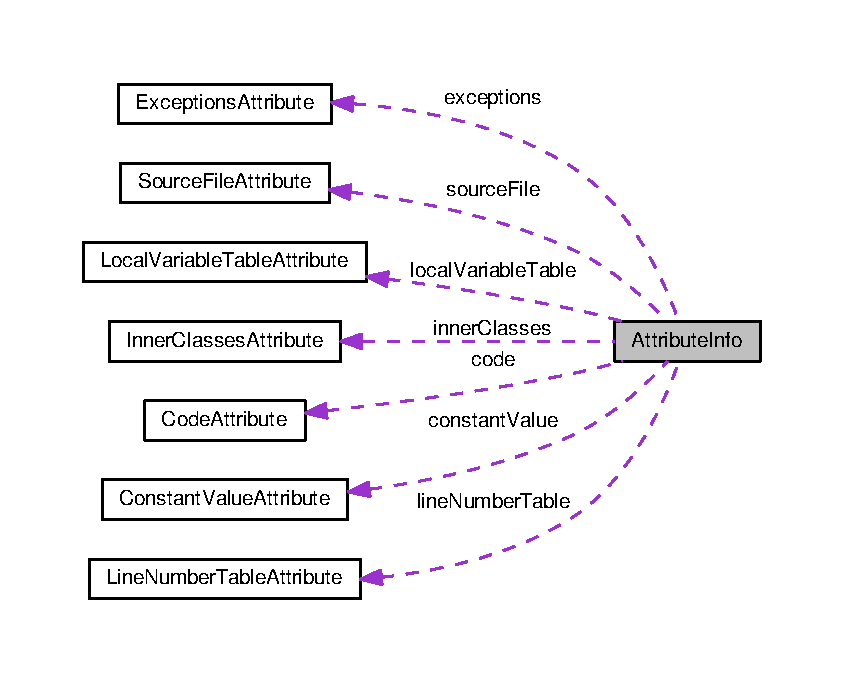
\includegraphics[width=350pt]{classAttributeInfo__coll__graph}
\end{center}
\end{figure}
\subsection*{Classes}
\begin{DoxyCompactItemize}
\item 
class \hyperlink{classAttributeInfo_1_1read}{read}
\begin{DoxyCompactList}\small\item\em Método que visa armazenar os valores das informações dos atributos. \end{DoxyCompactList}\end{DoxyCompactItemize}
\subsection*{Public Member Functions}
\begin{DoxyCompactItemize}
\item 
void {\bfseries read} (F\+I\+LE $\ast$, vector$<$ \hyperlink{classCPInfo}{C\+P\+Info} $\ast$ $>$)\hypertarget{classAttributeInfo_a3413daa38334773b032fb1b5298f9acc}{}\label{classAttributeInfo_a3413daa38334773b032fb1b5298f9acc}

\item 
void {\bfseries print} (vector$<$ \hyperlink{classCPInfo}{C\+P\+Info} $\ast$ $>$)\hypertarget{classAttributeInfo_a26dfac9d4fedf0aff08f76240f0e0180}{}\label{classAttributeInfo_a26dfac9d4fedf0aff08f76240f0e0180}

\item 
uint16\+\_\+t {\bfseries get\+Attribute\+Name\+Index} ()\hypertarget{classAttributeInfo_a9392cd3c3328782129745e842bba41b2}{}\label{classAttributeInfo_a9392cd3c3328782129745e842bba41b2}

\item 
uint16\+\_\+t {\bfseries get\+Attribute\+Length} ()\hypertarget{classAttributeInfo_a83e305b84d94ddaa200e905fcc6ca930}{}\label{classAttributeInfo_a83e305b84d94ddaa200e905fcc6ca930}

\item 
\hyperlink{classConstantValueAttribute}{Constant\+Value\+Attribute} {\bfseries get\+Constant\+Value\+Attribute} ()\hypertarget{classAttributeInfo_a405c8c2996e138315965ea4e20f83b84}{}\label{classAttributeInfo_a405c8c2996e138315965ea4e20f83b84}

\item 
\hyperlink{classCodeAttribute}{Code\+Attribute} {\bfseries get\+Code\+Attribute} ()\hypertarget{classAttributeInfo_a5c3822d70b765e9f0785c4ec7e0c7853}{}\label{classAttributeInfo_a5c3822d70b765e9f0785c4ec7e0c7853}

\item 
\hyperlink{classInnerClassesAttribute}{Inner\+Classes\+Attribute} {\bfseries get\+Inner\+Classes\+Attribute} ()\hypertarget{classAttributeInfo_ab0bb0de40d838b4bb52a5da708d0f6a6}{}\label{classAttributeInfo_ab0bb0de40d838b4bb52a5da708d0f6a6}

\item 
\hyperlink{classSourceFileAttribute}{Source\+File\+Attribute} {\bfseries get\+Source\+File\+Attribute} ()\hypertarget{classAttributeInfo_a09cdb336a64159e0f93ffe73b064e01c}{}\label{classAttributeInfo_a09cdb336a64159e0f93ffe73b064e01c}

\item 
\hyperlink{classLineNumberTableAttribute}{Line\+Number\+Table\+Attribute} {\bfseries get\+Line\+Number\+Table\+Attribute} ()\hypertarget{classAttributeInfo_a17bc4e1435137d714da8942171f82012}{}\label{classAttributeInfo_a17bc4e1435137d714da8942171f82012}

\item 
\hyperlink{classLocalVariableTableAttribute}{Local\+Variable\+Table\+Attribute} {\bfseries get\+Local\+Variable\+Table\+Attribute} ()\hypertarget{classAttributeInfo_a916735dc9f933dbc80ac4e7d61a07768}{}\label{classAttributeInfo_a916735dc9f933dbc80ac4e7d61a07768}

\item 
\hyperlink{classExceptionsAttribute}{Exceptions\+Attribute} {\bfseries get\+Exceptions\+Attribute} ()\hypertarget{classAttributeInfo_a0b0f4877987a0ce9eebe156871afe2d7}{}\label{classAttributeInfo_a0b0f4877987a0ce9eebe156871afe2d7}

\end{DoxyCompactItemize}


\subsection{Detailed Description}
Classe que contém as informações dos atributos. 

\begin{DoxyRefDesc}{Bug}
\item[\hyperlink{bug__bug000013}{Bug}]No known bugs. \end{DoxyRefDesc}


The documentation for this class was generated from the following files\+:\begin{DoxyCompactItemize}
\item 
/home/arturhbs/\+Documentos/unb/8 semestre/\+S\+B/\+J\+V\+M/src/hpp/\hyperlink{AttributeInfo_8hpp}{Attribute\+Info.\+hpp}\item 
/home/arturhbs/\+Documentos/unb/8 semestre/\+S\+B/\+J\+V\+M/src/cpp/\hyperlink{AttributeInfo_8cpp}{Attribute\+Info.\+cpp}\end{DoxyCompactItemize}

\hypertarget{classByteReader}{}\section{Byte\+Reader$<$ T $>$ Class Template Reference}
\label{classByteReader}\index{Byte\+Reader$<$ T $>$@{Byte\+Reader$<$ T $>$}}


Contém o método byte\+Catch -\/ busca fazer a leitura dos bytes do .class;.  




{\ttfamily \#include $<$Byte\+Reader.\+hpp$>$}

\subsection*{Public Member Functions}
\begin{DoxyCompactItemize}
\item 
T {\bfseries byte\+Catch} (F\+I\+LE $\ast$fp)\hypertarget{classByteReader_ae570748805994596f51ae033183935d7}{}\label{classByteReader_ae570748805994596f51ae033183935d7}

\end{DoxyCompactItemize}


\subsection{Detailed Description}
\subsubsection*{template$<$class T$>$\\*
class Byte\+Reader$<$ T $>$}

Contém o método byte\+Catch -\/ busca fazer a leitura dos bytes do .class;. 

\begin{DoxyRefDesc}{Bug}
\item[\hyperlink{bug__bug000015}{Bug}]No known bugs. \end{DoxyRefDesc}


The documentation for this class was generated from the following file\+:\begin{DoxyCompactItemize}
\item 
/home/arturhbs/\+Documentos/unb/8 semestre/\+S\+B/\+J\+V\+M/src/hpp/\hyperlink{ByteReader_8hpp}{Byte\+Reader.\+hpp}\end{DoxyCompactItemize}

\hypertarget{classClassFile}{}\section{Class\+File Class Reference}
\label{classClassFile}\index{Class\+File@{Class\+File}}
\subsection*{Public Member Functions}
\begin{DoxyCompactItemize}
\item 
{\bfseries Class\+File} (F\+I\+LE $\ast$fp)\hypertarget{classClassFile_aed7c4bc94d4d7aff8785a262befa19fc}{}\label{classClassFile_aed7c4bc94d4d7aff8785a262befa19fc}

\item 
uint32\+\_\+t {\bfseries get\+Magic} ()\hypertarget{classClassFile_a7b981e486aada980cf8aa77669f4f578}{}\label{classClassFile_a7b981e486aada980cf8aa77669f4f578}

\item 
uint16\+\_\+t {\bfseries get\+Major\+Version} ()\hypertarget{classClassFile_aecde28e5d51413a4f1856385e0a2c642}{}\label{classClassFile_aecde28e5d51413a4f1856385e0a2c642}

\item 
uint16\+\_\+t {\bfseries get\+Minor\+Version} ()\hypertarget{classClassFile_a98a3170782cb82940f317f06f90c9398}{}\label{classClassFile_a98a3170782cb82940f317f06f90c9398}

\item 
uint16\+\_\+t {\bfseries get\+Constant\+Pool\+Count} ()\hypertarget{classClassFile_a72ea0eac7a8252056ee0c615afcd76fc}{}\label{classClassFile_a72ea0eac7a8252056ee0c615afcd76fc}

\item 
vector$<$ \hyperlink{classCPInfo}{C\+P\+Info} $\ast$ $>$ {\bfseries get\+Constant\+Pool} ()\hypertarget{classClassFile_a6268c973fcaf6247f7fe338f3ee54d7a}{}\label{classClassFile_a6268c973fcaf6247f7fe338f3ee54d7a}

\item 
uint16\+\_\+t {\bfseries get\+Access\+Flags} ()\hypertarget{classClassFile_a0426eeb52b8bcd0dfbee9dcaf368ad09}{}\label{classClassFile_a0426eeb52b8bcd0dfbee9dcaf368ad09}

\item 
uint16\+\_\+t {\bfseries get\+This\+Class} ()\hypertarget{classClassFile_a54c12b8a159a7952c668c094df9a6862}{}\label{classClassFile_a54c12b8a159a7952c668c094df9a6862}

\item 
uint16\+\_\+t {\bfseries get\+Super\+Class} ()\hypertarget{classClassFile_a3fe451508fa72823e9d2879e82257d71}{}\label{classClassFile_a3fe451508fa72823e9d2879e82257d71}

\item 
uint16\+\_\+t {\bfseries get\+Interfaces\+Count} ()\hypertarget{classClassFile_a959e59776547f71b8596f7ac21ade1a8}{}\label{classClassFile_a959e59776547f71b8596f7ac21ade1a8}

\item 
vector$<$ \hyperlink{classInterfaceInfo}{Interface\+Info} $\ast$ $>$ {\bfseries get\+Interfaces} ()\hypertarget{classClassFile_a1b0d4ceab8ba1bacf48167e34d9f9697}{}\label{classClassFile_a1b0d4ceab8ba1bacf48167e34d9f9697}

\item 
uint16\+\_\+t {\bfseries get\+Fields\+Count} ()\hypertarget{classClassFile_ad222ea747904bb555c9b75adea49b946}{}\label{classClassFile_ad222ea747904bb555c9b75adea49b946}

\item 
vector$<$ \hyperlink{classFieldInfo}{Field\+Info} $\ast$ $>$ {\bfseries get\+Fields} ()\hypertarget{classClassFile_ab176b9637fc6030553a2dd427a128065}{}\label{classClassFile_ab176b9637fc6030553a2dd427a128065}

\item 
uint16\+\_\+t {\bfseries get\+Methods\+Count} ()\hypertarget{classClassFile_ab39d5edd6b3f994b4d5027cce4cf535f}{}\label{classClassFile_ab39d5edd6b3f994b4d5027cce4cf535f}

\item 
vector$<$ \hyperlink{classMethodInfo}{Method\+Info} $\ast$ $>$ {\bfseries get\+Methods} ()\hypertarget{classClassFile_a14c4a6ac978652a94720c111b47e2aa3}{}\label{classClassFile_a14c4a6ac978652a94720c111b47e2aa3}

\item 
uint16\+\_\+t {\bfseries get\+Attributes\+Count} ()\hypertarget{classClassFile_a959c28000c2602eca1414f910c720932}{}\label{classClassFile_a959c28000c2602eca1414f910c720932}

\item 
\hyperlink{classAttributeInfo}{Attribute\+Info} $\ast$ {\bfseries get\+Attributes} ()\hypertarget{classClassFile_a693c990aaba0c4c0df17bd6d54167c8d}{}\label{classClassFile_a693c990aaba0c4c0df17bd6d54167c8d}

\end{DoxyCompactItemize}
\subsection*{Static Public Attributes}
\begin{DoxyCompactItemize}
\item 
static const uint32\+\_\+t {\bfseries M\+A\+G\+I\+C\+\_\+\+N\+U\+M\+B\+ER} = 0x\+C\+A\+F\+E\+B\+A\+BE\hypertarget{classClassFile_a9a86c1e3bad5aa1fbe7f62b8c8894e83}{}\label{classClassFile_a9a86c1e3bad5aa1fbe7f62b8c8894e83}

\item 
static const uint16\+\_\+t {\bfseries A\+C\+C\+\_\+\+P\+U\+B\+L\+IC} = 0x0001\hypertarget{classClassFile_a136f640c12cd31d174fed27de55d9e67}{}\label{classClassFile_a136f640c12cd31d174fed27de55d9e67}

\item 
static const uint16\+\_\+t {\bfseries A\+C\+C\+\_\+\+F\+I\+N\+AL} = 0x0010\hypertarget{classClassFile_a284d6715a2914d845a878e7940dded2c}{}\label{classClassFile_a284d6715a2914d845a878e7940dded2c}

\item 
static const uint16\+\_\+t {\bfseries A\+C\+C\+\_\+\+S\+U\+P\+ER} = 0x0020\hypertarget{classClassFile_a8cecc64f1a1eba284639bf5ddcbda370}{}\label{classClassFile_a8cecc64f1a1eba284639bf5ddcbda370}

\item 
static const uint16\+\_\+t {\bfseries A\+C\+C\+\_\+\+I\+N\+T\+E\+R\+F\+A\+CE} = 0x0200\hypertarget{classClassFile_a58b40cee61b30f9226f826f88a7d3c2c}{}\label{classClassFile_a58b40cee61b30f9226f826f88a7d3c2c}

\item 
static const uint16\+\_\+t {\bfseries A\+C\+C\+\_\+\+A\+B\+S\+T\+R\+A\+CT} = 0x0400\hypertarget{classClassFile_a3a35282d757e38fccb2a4ae666455072}{}\label{classClassFile_a3a35282d757e38fccb2a4ae666455072}

\item 
static const uint16\+\_\+t {\bfseries A\+C\+C\+\_\+\+S\+Y\+N\+T\+H\+E\+T\+IC} = 0x1000\hypertarget{classClassFile_ab60ec9df262c29d110276482c72f557c}{}\label{classClassFile_ab60ec9df262c29d110276482c72f557c}

\item 
static const uint16\+\_\+t {\bfseries A\+C\+C\+\_\+\+A\+N\+N\+O\+T\+A\+T\+I\+ON} = 0x2000\hypertarget{classClassFile_ad37162e7b480660fab7ec2d33936f713}{}\label{classClassFile_ad37162e7b480660fab7ec2d33936f713}

\item 
static const uint16\+\_\+t {\bfseries A\+C\+C\+\_\+\+E\+N\+UM} = 0x4000\hypertarget{classClassFile_a1da2677a7301fea5c447dd8cdcb412b0}{}\label{classClassFile_a1da2677a7301fea5c447dd8cdcb412b0}

\end{DoxyCompactItemize}


The documentation for this class was generated from the following files\+:\begin{DoxyCompactItemize}
\item 
/home/arturhbs/\+Documentos/unb/8 semestre/\+S\+B/\+J\+V\+M/src/hpp/Class\+File.\+hpp\item 
/home/arturhbs/\+Documentos/unb/8 semestre/\+S\+B/\+J\+V\+M/src/cpp/Class\+File.\+cpp\end{DoxyCompactItemize}

\hypertarget{classClassInfo}{}\section{Class\+Info Class Reference}
\label{classClassInfo}\index{Class\+Info@{Class\+Info}}


Classe que contém as informações gerais das classes.  




{\ttfamily \#include $<$Attribute\+Info.\+hpp$>$}

\subsection*{Public Member Functions}
\begin{DoxyCompactItemize}
\item 
void {\bfseries read} (F\+I\+LE $\ast$fp)\hypertarget{classClassInfo_ad2e55dfb641367a6f07cbc9a5fee931b}{}\label{classClassInfo_ad2e55dfb641367a6f07cbc9a5fee931b}

\item 
uint16\+\_\+t {\bfseries get\+Inner\+Class\+Info\+Index} ()\hypertarget{classClassInfo_a6355f698a36e546ab8a83aebdd02deaa}{}\label{classClassInfo_a6355f698a36e546ab8a83aebdd02deaa}

\item 
uint16\+\_\+t {\bfseries get\+Outer\+Class\+Info\+Index} ()\hypertarget{classClassInfo_a89d3d35fe30b9846ff6907be50e86b29}{}\label{classClassInfo_a89d3d35fe30b9846ff6907be50e86b29}

\item 
uint16\+\_\+t {\bfseries get\+Inner\+Name\+Index} ()\hypertarget{classClassInfo_a38075d61d6812ecf422de434aa11bb01}{}\label{classClassInfo_a38075d61d6812ecf422de434aa11bb01}

\item 
uint16\+\_\+t {\bfseries get\+Inner\+Class\+Access\+Flags} ()\hypertarget{classClassInfo_a3e09735f9005ba692b86fbde0417b17f}{}\label{classClassInfo_a3e09735f9005ba692b86fbde0417b17f}

\end{DoxyCompactItemize}


\subsection{Detailed Description}
Classe que contém as informações gerais das classes. 

The documentation for this class was generated from the following files\+:\begin{DoxyCompactItemize}
\item 
/home/arturhbs/\+Documentos/unb/8 semestre/\+S\+B/\+J\+V\+M/src/hpp/\hyperlink{AttributeInfo_8hpp}{Attribute\+Info.\+hpp}\item 
/home/arturhbs/\+Documentos/unb/8 semestre/\+S\+B/\+J\+V\+M/src/cpp/Attribute\+Info.\+cpp\end{DoxyCompactItemize}

\hypertarget{classClassLoader}{}\section{Class\+Loader Class Reference}
\label{classClassLoader}\index{Class\+Loader@{Class\+Loader}}


Classe que armazena o caminho para o arquivo .class e separa o \hyperlink{classMethodArea}{Method\+Area};.  




{\ttfamily \#include $<$Class\+Loader.\+hpp$>$}

\subsection*{Classes}
\begin{DoxyCompactItemize}
\item 
class \hyperlink{classClassLoader_1_1loadClassFile}{load\+Class\+File}
\begin{DoxyCompactList}\small\item\em Método que visa carregar o arquivo .class. \end{DoxyCompactList}\item 
class \hyperlink{classClassLoader_1_1loadSuperClasses}{load\+Super\+Classes}
\begin{DoxyCompactList}\small\item\em Método que visa carregar as super\+Classes o arquivo .class. \end{DoxyCompactList}\end{DoxyCompactItemize}
\subsection*{Public Member Functions}
\begin{DoxyCompactItemize}
\item 
\hyperlink{classClassLoader_a33dea7f5288f739017d61d462b935506}{Class\+Loader} (string)
\begin{DoxyCompactList}\small\item\em Construtor \hyperlink{classClassLoader}{Class\+Loader}. \end{DoxyCompactList}\item 
\hyperlink{classClassFile}{Class\+File} {\bfseries load\+Class\+File} (string)\hypertarget{classClassLoader_a368e94d895b9e99c66e9b39dd7025e67}{}\label{classClassLoader_a368e94d895b9e99c66e9b39dd7025e67}

\item 
void {\bfseries load\+Super\+Classes} (\hyperlink{classClassFile}{Class\+File} $\ast$)\hypertarget{classClassLoader_ad704891933608240ea282e835e92aaa2}{}\label{classClassLoader_ad704891933608240ea282e835e92aaa2}

\item 
void {\bfseries set\+Method\+Area} (\hyperlink{classMethodArea}{Method\+Area} $\ast$method\+Area)\hypertarget{classClassLoader_a3f432b26ce13cd17da2986320b6060c8}{}\label{classClassLoader_a3f432b26ce13cd17da2986320b6060c8}

\item 
\hyperlink{classClassFile}{Class\+File} $\ast$ {\bfseries get\+Class\+From\+Method\+Area} (string class\+Name)\hypertarget{classClassLoader_ac792ecbaa98738fddee0c4285759ce2c}{}\label{classClassLoader_ac792ecbaa98738fddee0c4285759ce2c}

\item 
\hyperlink{classMethodArea}{Method\+Area} $\ast$ {\bfseries get\+Method\+Area} ()\hypertarget{classClassLoader_a2a28f4514a3223fa4534d5dccd12612c}{}\label{classClassLoader_a2a28f4514a3223fa4534d5dccd12612c}

\end{DoxyCompactItemize}


\subsection{Detailed Description}
Classe que armazena o caminho para o arquivo .class e separa o \hyperlink{classMethodArea}{Method\+Area};. 

\subsection{Constructor \& Destructor Documentation}
\index{Class\+Loader@{Class\+Loader}!Class\+Loader@{Class\+Loader}}
\index{Class\+Loader@{Class\+Loader}!Class\+Loader@{Class\+Loader}}
\subsubsection[{\texorpdfstring{Class\+Loader(string)}{ClassLoader(string)}}]{\setlength{\rightskip}{0pt plus 5cm}Class\+Loader\+::\+Class\+Loader (
\begin{DoxyParamCaption}
\item[{string}]{project\+Path}
\end{DoxyParamCaption}
)}\hypertarget{classClassLoader_a33dea7f5288f739017d61d462b935506}{}\label{classClassLoader_a33dea7f5288f739017d61d462b935506}


Construtor \hyperlink{classClassLoader}{Class\+Loader}. 


\begin{DoxyParams}{Parameters}
{\em project\+Path} & \\
\hline
\end{DoxyParams}
\begin{DoxyReturn}{Returns}

\end{DoxyReturn}


The documentation for this class was generated from the following files\+:\begin{DoxyCompactItemize}
\item 
/home/arturhbs/\+Documentos/unb/8 semestre/\+S\+B/\+J\+V\+M/src/hpp/Class\+Loader.\+hpp\item 
/home/arturhbs/\+Documentos/unb/8 semestre/\+S\+B/\+J\+V\+M/src/cpp/\hyperlink{ClassLoader_8cpp}{Class\+Loader.\+cpp}\end{DoxyCompactItemize}

\hypertarget{classClassPrinter}{}\section{Class\+Printer Class Reference}
\label{classClassPrinter}\index{Class\+Printer@{Class\+Printer}}


classe que contém a chamada de todos os métodos que visam mostrar na tela os campos do class\+File;  




{\ttfamily \#include $<$Class\+Printer.\+hpp$>$}

\subsection*{Public Member Functions}
\begin{DoxyCompactItemize}
\item 
{\bfseries Class\+Printer} (\hyperlink{classClassFile}{Class\+File} class\+File, \hyperlink{classInstructionSet}{Instruction\+Set} $\ast$instruction\+Set)\hypertarget{classClassPrinter_ae6f4be2efe9a9e3e6056304330dc7430}{}\label{classClassPrinter_ae6f4be2efe9a9e3e6056304330dc7430}

\item 
void {\bfseries print} ()\hypertarget{classClassPrinter_a8871ec5a8e14410486d1aa1fa93323eb}{}\label{classClassPrinter_a8871ec5a8e14410486d1aa1fa93323eb}

\item 
string {\bfseries Flag\+\_\+names} (int flag\+\_\+byte, int parametro)\hypertarget{classClassPrinter_a9883cb947ce417ffe130175a93d9fd32}{}\label{classClassPrinter_a9883cb947ce417ffe130175a93d9fd32}

\end{DoxyCompactItemize}


\subsection{Detailed Description}
classe que contém a chamada de todos os métodos que visam mostrar na tela os campos do class\+File; 

The documentation for this class was generated from the following files\+:\begin{DoxyCompactItemize}
\item 
/home/arturhbs/\+Documentos/unb/8 semestre/\+S\+B/\+J\+V\+M/src/hpp/\hyperlink{ClassPrinter_8hpp}{Class\+Printer.\+hpp}\item 
/home/arturhbs/\+Documentos/unb/8 semestre/\+S\+B/\+J\+V\+M/src/cpp/\hyperlink{ClassPrinter_8cpp}{Class\+Printer.\+cpp}\end{DoxyCompactItemize}

\hypertarget{classCodeAttribute}{}\section{Code\+Attribute Class Reference}
\label{classCodeAttribute}\index{Code\+Attribute@{Code\+Attribute}}


Classe que consiste em armazenar as informações dos atributos.  




{\ttfamily \#include $<$Attribute\+Info.\+hpp$>$}

\subsection*{Classes}
\begin{DoxyCompactItemize}
\item 
class \hyperlink{classCodeAttribute_1_1read}{read}
\begin{DoxyCompactList}\small\item\em Método que visa armazenar os valores dos code dos atributos. \end{DoxyCompactList}\end{DoxyCompactItemize}
\subsection*{Public Member Functions}
\begin{DoxyCompactItemize}
\item 
void {\bfseries read} (F\+I\+LE $\ast$, vector$<$ \hyperlink{classCPInfo}{C\+P\+Info} $\ast$ $>$)\hypertarget{classCodeAttribute_acb8378aad8421371b26442ffbf778de4}{}\label{classCodeAttribute_acb8378aad8421371b26442ffbf778de4}

\item 
uint16\+\_\+t {\bfseries get\+Max\+Stack} ()\hypertarget{classCodeAttribute_a9eb6a6b7bd7bd870f745bc089d407e45}{}\label{classCodeAttribute_a9eb6a6b7bd7bd870f745bc089d407e45}

\item 
uint16\+\_\+t {\bfseries get\+Max\+Locals} ()\hypertarget{classCodeAttribute_aa97ceb04d99e607389a4cf08b3b65db1}{}\label{classCodeAttribute_aa97ceb04d99e607389a4cf08b3b65db1}

\item 
uint32\+\_\+t {\bfseries get\+Code\+Length} ()\hypertarget{classCodeAttribute_ae365ff1b5fc98df49f3f61379d59978f}{}\label{classCodeAttribute_ae365ff1b5fc98df49f3f61379d59978f}

\item 
uint8\+\_\+t $\ast$ {\bfseries get\+Code} ()\hypertarget{classCodeAttribute_a713d99a501cb88c344013b5820ea6e8b}{}\label{classCodeAttribute_a713d99a501cb88c344013b5820ea6e8b}

\item 
uint16\+\_\+t {\bfseries get\+Exception\+Table\+Length} ()\hypertarget{classCodeAttribute_a4a1408612b357305d2c27673d8e18124}{}\label{classCodeAttribute_a4a1408612b357305d2c27673d8e18124}

\item 
\hyperlink{classExceptionHandler}{Exception\+Handler} $\ast$ {\bfseries get\+Exception\+Table} ()\hypertarget{classCodeAttribute_a7905efeeb4bbdd57cc07605757372db5}{}\label{classCodeAttribute_a7905efeeb4bbdd57cc07605757372db5}

\item 
uint16\+\_\+t {\bfseries get\+Attributes\+Count} ()\hypertarget{classCodeAttribute_a795890e641c508602f2b842af5779fc6}{}\label{classCodeAttribute_a795890e641c508602f2b842af5779fc6}

\item 
\hyperlink{classAttributeInfo}{Attribute\+Info} $\ast$ {\bfseries get\+Attributes} ()\hypertarget{classCodeAttribute_a5f36ae9a19d451dbb7c1aedad06454ff}{}\label{classCodeAttribute_a5f36ae9a19d451dbb7c1aedad06454ff}

\end{DoxyCompactItemize}


\subsection{Detailed Description}
Classe que consiste em armazenar as informações dos atributos. 

\begin{DoxyRefDesc}{Bug}
\item[\hyperlink{bug__bug000004}{Bug}]No known bugs. \end{DoxyRefDesc}


The documentation for this class was generated from the following files\+:\begin{DoxyCompactItemize}
\item 
/home/arturhbs/\+Documentos/unb/8 semestre/\+S\+B/\+J\+V\+M/src/hpp/\hyperlink{AttributeInfo_8hpp}{Attribute\+Info.\+hpp}\item 
/home/arturhbs/\+Documentos/unb/8 semestre/\+S\+B/\+J\+V\+M/src/cpp/\hyperlink{AttributeInfo_8cpp}{Attribute\+Info.\+cpp}\end{DoxyCompactItemize}

\hypertarget{structConstantClassInfo}{}\section{Constant\+Class\+Info Struct Reference}
\label{structConstantClassInfo}\index{Constant\+Class\+Info@{Constant\+Class\+Info}}
\subsection*{Public Attributes}
\begin{DoxyCompactItemize}
\item 
uint16\+\_\+t {\bfseries name\+\_\+index}\hypertarget{structConstantClassInfo_a691eabaa91856df4e408425764b9515e}{}\label{structConstantClassInfo_a691eabaa91856df4e408425764b9515e}

\end{DoxyCompactItemize}


The documentation for this struct was generated from the following file\+:\begin{DoxyCompactItemize}
\item 
/home/arturhbs/\+Documentos/unb/8 semestre/\+S\+B/\+J\+V\+M/src/hpp/C\+P\+Info.\+hpp\end{DoxyCompactItemize}

\hypertarget{structConstantDoubleInfo}{}\section{Constant\+Double\+Info Struct Reference}
\label{structConstantDoubleInfo}\index{Constant\+Double\+Info@{Constant\+Double\+Info}}
\subsection*{Public Attributes}
\begin{DoxyCompactItemize}
\item 
uint32\+\_\+t {\bfseries high\+\_\+bytes}\hypertarget{structConstantDoubleInfo_a4390f86345cd246c4ffbb2f76fe2783d}{}\label{structConstantDoubleInfo_a4390f86345cd246c4ffbb2f76fe2783d}

\item 
uint32\+\_\+t {\bfseries low\+\_\+bytes}\hypertarget{structConstantDoubleInfo_a5559dde9df215499faab8d2e409e0044}{}\label{structConstantDoubleInfo_a5559dde9df215499faab8d2e409e0044}

\end{DoxyCompactItemize}


The documentation for this struct was generated from the following file\+:\begin{DoxyCompactItemize}
\item 
/home/arturhbs/\+Documentos/unb/8 semestre/\+S\+B/\+J\+V\+M/src/hpp/C\+P\+Info.\+hpp\end{DoxyCompactItemize}

\hypertarget{structConstantFieldrefInfo}{}\section{Constant\+Fieldref\+Info Struct Reference}
\label{structConstantFieldrefInfo}\index{Constant\+Fieldref\+Info@{Constant\+Fieldref\+Info}}
\subsection*{Public Attributes}
\begin{DoxyCompactItemize}
\item 
uint16\+\_\+t {\bfseries class\+\_\+index}\hypertarget{structConstantFieldrefInfo_a7ea01fdcbde2bcbc719a5c5834936082}{}\label{structConstantFieldrefInfo_a7ea01fdcbde2bcbc719a5c5834936082}

\item 
uint16\+\_\+t {\bfseries name\+\_\+and\+\_\+type\+\_\+index}\hypertarget{structConstantFieldrefInfo_a28acf39ab3393b29ebe328bb37021729}{}\label{structConstantFieldrefInfo_a28acf39ab3393b29ebe328bb37021729}

\end{DoxyCompactItemize}


The documentation for this struct was generated from the following file\+:\begin{DoxyCompactItemize}
\item 
/home/arturhbs/\+Documentos/unb/8 semestre/\+S\+B/\+J\+V\+M/src/hpp/C\+P\+Info.\+hpp\end{DoxyCompactItemize}

\hypertarget{structConstantFloatInfo}{}\section{Constant\+Float\+Info Struct Reference}
\label{structConstantFloatInfo}\index{Constant\+Float\+Info@{Constant\+Float\+Info}}
\subsection*{Public Attributes}
\begin{DoxyCompactItemize}
\item 
uint32\+\_\+t {\bfseries bytes}\hypertarget{structConstantFloatInfo_a73fe6845d0616920001d18e68c8a228b}{}\label{structConstantFloatInfo_a73fe6845d0616920001d18e68c8a228b}

\end{DoxyCompactItemize}


The documentation for this struct was generated from the following file\+:\begin{DoxyCompactItemize}
\item 
/home/arturhbs/\+Documentos/unb/8 semestre/\+S\+B/\+J\+V\+M/src/hpp/C\+P\+Info.\+hpp\end{DoxyCompactItemize}

\hypertarget{structConstantIntegerInfo}{}\section{Constant\+Integer\+Info Struct Reference}
\label{structConstantIntegerInfo}\index{Constant\+Integer\+Info@{Constant\+Integer\+Info}}
\subsection*{Public Attributes}
\begin{DoxyCompactItemize}
\item 
uint32\+\_\+t {\bfseries bytes}\hypertarget{structConstantIntegerInfo_a809111b4b66377eb519a645632f7114a}{}\label{structConstantIntegerInfo_a809111b4b66377eb519a645632f7114a}

\end{DoxyCompactItemize}


The documentation for this struct was generated from the following file\+:\begin{DoxyCompactItemize}
\item 
/home/arturhbs/\+Documentos/unb/8 semestre/\+S\+B/\+J\+V\+M/src/hpp/C\+P\+Info.\+hpp\end{DoxyCompactItemize}

\hypertarget{structConstantInterfaceMethodrefInfo}{}\section{Constant\+Interface\+Methodref\+Info Struct Reference}
\label{structConstantInterfaceMethodrefInfo}\index{Constant\+Interface\+Methodref\+Info@{Constant\+Interface\+Methodref\+Info}}
\subsection*{Public Attributes}
\begin{DoxyCompactItemize}
\item 
uint16\+\_\+t {\bfseries class\+\_\+index}\hypertarget{structConstantInterfaceMethodrefInfo_aa247e63af32e9dfdb7ab9a76dcfbc679}{}\label{structConstantInterfaceMethodrefInfo_aa247e63af32e9dfdb7ab9a76dcfbc679}

\item 
uint16\+\_\+t {\bfseries name\+\_\+and\+\_\+type\+\_\+index}\hypertarget{structConstantInterfaceMethodrefInfo_a876fd6bf106f42e54e35ff401e61b88b}{}\label{structConstantInterfaceMethodrefInfo_a876fd6bf106f42e54e35ff401e61b88b}

\end{DoxyCompactItemize}


The documentation for this struct was generated from the following file\+:\begin{DoxyCompactItemize}
\item 
/home/arturhbs/\+Documentos/unb/8 semestre/\+S\+B/\+J\+V\+M/src/hpp/C\+P\+Info.\+hpp\end{DoxyCompactItemize}

\hypertarget{structConstantInvokeDynamicInfo}{}\section{Constant\+Invoke\+Dynamic\+Info Struct Reference}
\label{structConstantInvokeDynamicInfo}\index{Constant\+Invoke\+Dynamic\+Info@{Constant\+Invoke\+Dynamic\+Info}}
\subsection*{Public Attributes}
\begin{DoxyCompactItemize}
\item 
uint16\+\_\+t {\bfseries bootstrap\+\_\+method\+\_\+attr\+\_\+index}\hypertarget{structConstantInvokeDynamicInfo_a8e5bd368ad9065219095b4dba2c757e0}{}\label{structConstantInvokeDynamicInfo_a8e5bd368ad9065219095b4dba2c757e0}

\item 
uint16\+\_\+t {\bfseries name\+\_\+and\+\_\+type\+\_\+index}\hypertarget{structConstantInvokeDynamicInfo_a1455133fd2ed451ac27d38d7c289b4e4}{}\label{structConstantInvokeDynamicInfo_a1455133fd2ed451ac27d38d7c289b4e4}

\end{DoxyCompactItemize}


The documentation for this struct was generated from the following file\+:\begin{DoxyCompactItemize}
\item 
/home/arturhbs/\+Documentos/unb/8 semestre/\+S\+B/\+J\+V\+M/src/hpp/C\+P\+Info.\+hpp\end{DoxyCompactItemize}

\hypertarget{structConstantLongInfo}{}\section{Constant\+Long\+Info Struct Reference}
\label{structConstantLongInfo}\index{Constant\+Long\+Info@{Constant\+Long\+Info}}
\subsection*{Public Attributes}
\begin{DoxyCompactItemize}
\item 
uint32\+\_\+t {\bfseries high\+\_\+bytes}\hypertarget{structConstantLongInfo_acc5f4a27a7ebbeb036c095934ba2c661}{}\label{structConstantLongInfo_acc5f4a27a7ebbeb036c095934ba2c661}

\item 
uint32\+\_\+t {\bfseries low\+\_\+bytes}\hypertarget{structConstantLongInfo_afad1110f24748eaec3b0210c7cf014c3}{}\label{structConstantLongInfo_afad1110f24748eaec3b0210c7cf014c3}

\end{DoxyCompactItemize}


The documentation for this struct was generated from the following file\+:\begin{DoxyCompactItemize}
\item 
/home/arturhbs/\+Documentos/unb/8 semestre/\+S\+B/\+J\+V\+M/src/hpp/C\+P\+Info.\+hpp\end{DoxyCompactItemize}

\hypertarget{structConstantMethodHandleInfo}{}\section{Constant\+Method\+Handle\+Info Struct Reference}
\label{structConstantMethodHandleInfo}\index{Constant\+Method\+Handle\+Info@{Constant\+Method\+Handle\+Info}}
\subsection*{Public Attributes}
\begin{DoxyCompactItemize}
\item 
uint8\+\_\+t {\bfseries reference\+\_\+kind}\hypertarget{structConstantMethodHandleInfo_a19082afa217fc474c3d503bd131f57f4}{}\label{structConstantMethodHandleInfo_a19082afa217fc474c3d503bd131f57f4}

\item 
uint16\+\_\+t {\bfseries reference\+\_\+index}\hypertarget{structConstantMethodHandleInfo_a462157c35f7dbacfdb538d8b8ec387b3}{}\label{structConstantMethodHandleInfo_a462157c35f7dbacfdb538d8b8ec387b3}

\end{DoxyCompactItemize}


The documentation for this struct was generated from the following file\+:\begin{DoxyCompactItemize}
\item 
/home/arturhbs/\+Documentos/unb/8 semestre/\+S\+B/\+J\+V\+M/src/hpp/C\+P\+Info.\+hpp\end{DoxyCompactItemize}

\hypertarget{structConstantMethodrefInfo}{}\section{Constant\+Methodref\+Info Struct Reference}
\label{structConstantMethodrefInfo}\index{Constant\+Methodref\+Info@{Constant\+Methodref\+Info}}
\subsection*{Public Attributes}
\begin{DoxyCompactItemize}
\item 
uint16\+\_\+t {\bfseries class\+\_\+index}\hypertarget{structConstantMethodrefInfo_abfb8e54d37521bee9c139d65f90facab}{}\label{structConstantMethodrefInfo_abfb8e54d37521bee9c139d65f90facab}

\item 
uint16\+\_\+t {\bfseries name\+\_\+and\+\_\+type\+\_\+index}\hypertarget{structConstantMethodrefInfo_a975a0ae57988a9bccf68c75a4f6fee43}{}\label{structConstantMethodrefInfo_a975a0ae57988a9bccf68c75a4f6fee43}

\end{DoxyCompactItemize}


The documentation for this struct was generated from the following file\+:\begin{DoxyCompactItemize}
\item 
/home/arturhbs/\+Documentos/unb/8 semestre/\+S\+B/\+J\+V\+M/src/hpp/C\+P\+Info.\+hpp\end{DoxyCompactItemize}

\hypertarget{structConstantMethodTypeInfo}{}\section{Constant\+Method\+Type\+Info Struct Reference}
\label{structConstantMethodTypeInfo}\index{Constant\+Method\+Type\+Info@{Constant\+Method\+Type\+Info}}
\subsection*{Public Attributes}
\begin{DoxyCompactItemize}
\item 
uint16\+\_\+t {\bfseries descriptor\+\_\+index}\hypertarget{structConstantMethodTypeInfo_a2b6ca015e55ccfa9712a5d04132ecfa4}{}\label{structConstantMethodTypeInfo_a2b6ca015e55ccfa9712a5d04132ecfa4}

\end{DoxyCompactItemize}


The documentation for this struct was generated from the following file\+:\begin{DoxyCompactItemize}
\item 
/home/arturhbs/\+Documentos/unb/8 semestre/\+S\+B/\+J\+V\+M/src/hpp/C\+P\+Info.\+hpp\end{DoxyCompactItemize}

\hypertarget{structConstantNameAndTypeInfo}{}\section{Constant\+Name\+And\+Type\+Info Struct Reference}
\label{structConstantNameAndTypeInfo}\index{Constant\+Name\+And\+Type\+Info@{Constant\+Name\+And\+Type\+Info}}
\subsection*{Public Attributes}
\begin{DoxyCompactItemize}
\item 
uint16\+\_\+t {\bfseries name\+\_\+index}\hypertarget{structConstantNameAndTypeInfo_af856420a7554c2bcb679e5f63c2d7a56}{}\label{structConstantNameAndTypeInfo_af856420a7554c2bcb679e5f63c2d7a56}

\item 
uint16\+\_\+t {\bfseries descriptor\+\_\+index}\hypertarget{structConstantNameAndTypeInfo_a6e0af83874d65183ffc9dfd501f3ef44}{}\label{structConstantNameAndTypeInfo_a6e0af83874d65183ffc9dfd501f3ef44}

\end{DoxyCompactItemize}


The documentation for this struct was generated from the following file\+:\begin{DoxyCompactItemize}
\item 
/home/arturhbs/\+Documentos/unb/8 semestre/\+S\+B/\+J\+V\+M/src/hpp/C\+P\+Info.\+hpp\end{DoxyCompactItemize}

\hypertarget{structConstantStringInfo}{}\section{Constant\+String\+Info Struct Reference}
\label{structConstantStringInfo}\index{Constant\+String\+Info@{Constant\+String\+Info}}
\subsection*{Public Attributes}
\begin{DoxyCompactItemize}
\item 
uint16\+\_\+t {\bfseries string\+\_\+index}\hypertarget{structConstantStringInfo_af59c7cee9394d4c929ffc4c86e10599b}{}\label{structConstantStringInfo_af59c7cee9394d4c929ffc4c86e10599b}

\end{DoxyCompactItemize}


The documentation for this struct was generated from the following file\+:\begin{DoxyCompactItemize}
\item 
/home/arturhbs/\+Documentos/unb/8 semestre/\+S\+B/\+J\+V\+M/src/hpp/C\+P\+Info.\+hpp\end{DoxyCompactItemize}

\hypertarget{structConstantUTF8Info}{}\section{Constant\+U\+T\+F8\+Info Struct Reference}
\label{structConstantUTF8Info}\index{Constant\+U\+T\+F8\+Info@{Constant\+U\+T\+F8\+Info}}
\subsection*{Public Attributes}
\begin{DoxyCompactItemize}
\item 
uint16\+\_\+t {\bfseries length}\hypertarget{structConstantUTF8Info_af60c124996f482092bdc4c47b2e5931a}{}\label{structConstantUTF8Info_af60c124996f482092bdc4c47b2e5931a}

\item 
uint8\+\_\+t $\ast$ {\bfseries bytes}\hypertarget{structConstantUTF8Info_a9bdfe2b8aaec7d227068de9b646769ac}{}\label{structConstantUTF8Info_a9bdfe2b8aaec7d227068de9b646769ac}

\end{DoxyCompactItemize}


The documentation for this struct was generated from the following file\+:\begin{DoxyCompactItemize}
\item 
/home/arturhbs/\+Documentos/unb/8 semestre/\+S\+B/\+J\+V\+M/src/hpp/C\+P\+Info.\+hpp\end{DoxyCompactItemize}

\hypertarget{classConstantValueAttribute}{}\section{Constant\+Value\+Attribute Class Reference}
\label{classConstantValueAttribute}\index{Constant\+Value\+Attribute@{Constant\+Value\+Attribute}}
\subsection*{Public Member Functions}
\begin{DoxyCompactItemize}
\item 
void {\bfseries read} (F\+I\+LE $\ast$)\hypertarget{classConstantValueAttribute_a736510ad35810b8b06b7fed1065b5f9f}{}\label{classConstantValueAttribute_a736510ad35810b8b06b7fed1065b5f9f}

\item 
uint16\+\_\+t {\bfseries get\+Constant\+Value\+Index} ()\hypertarget{classConstantValueAttribute_ab8f66dc68583f523e052482f14e44c9d}{}\label{classConstantValueAttribute_ab8f66dc68583f523e052482f14e44c9d}

\end{DoxyCompactItemize}


The documentation for this class was generated from the following files\+:\begin{DoxyCompactItemize}
\item 
/home/arturhbs/\+Documentos/unb/8 semestre/\+S\+B/\+J\+V\+M/src/hpp/\hyperlink{AttributeInfo_8hpp}{Attribute\+Info.\+hpp}\item 
/home/arturhbs/\+Documentos/unb/8 semestre/\+S\+B/\+J\+V\+M/src/cpp/Attribute\+Info.\+cpp\end{DoxyCompactItemize}

\hypertarget{classCPInfo}{}\section{C\+P\+Info Class Reference}
\label{classCPInfo}\index{C\+P\+Info@{C\+P\+Info}}


Collaboration diagram for C\+P\+Info\+:\nopagebreak
\begin{figure}[H]
\begin{center}
\leavevmode
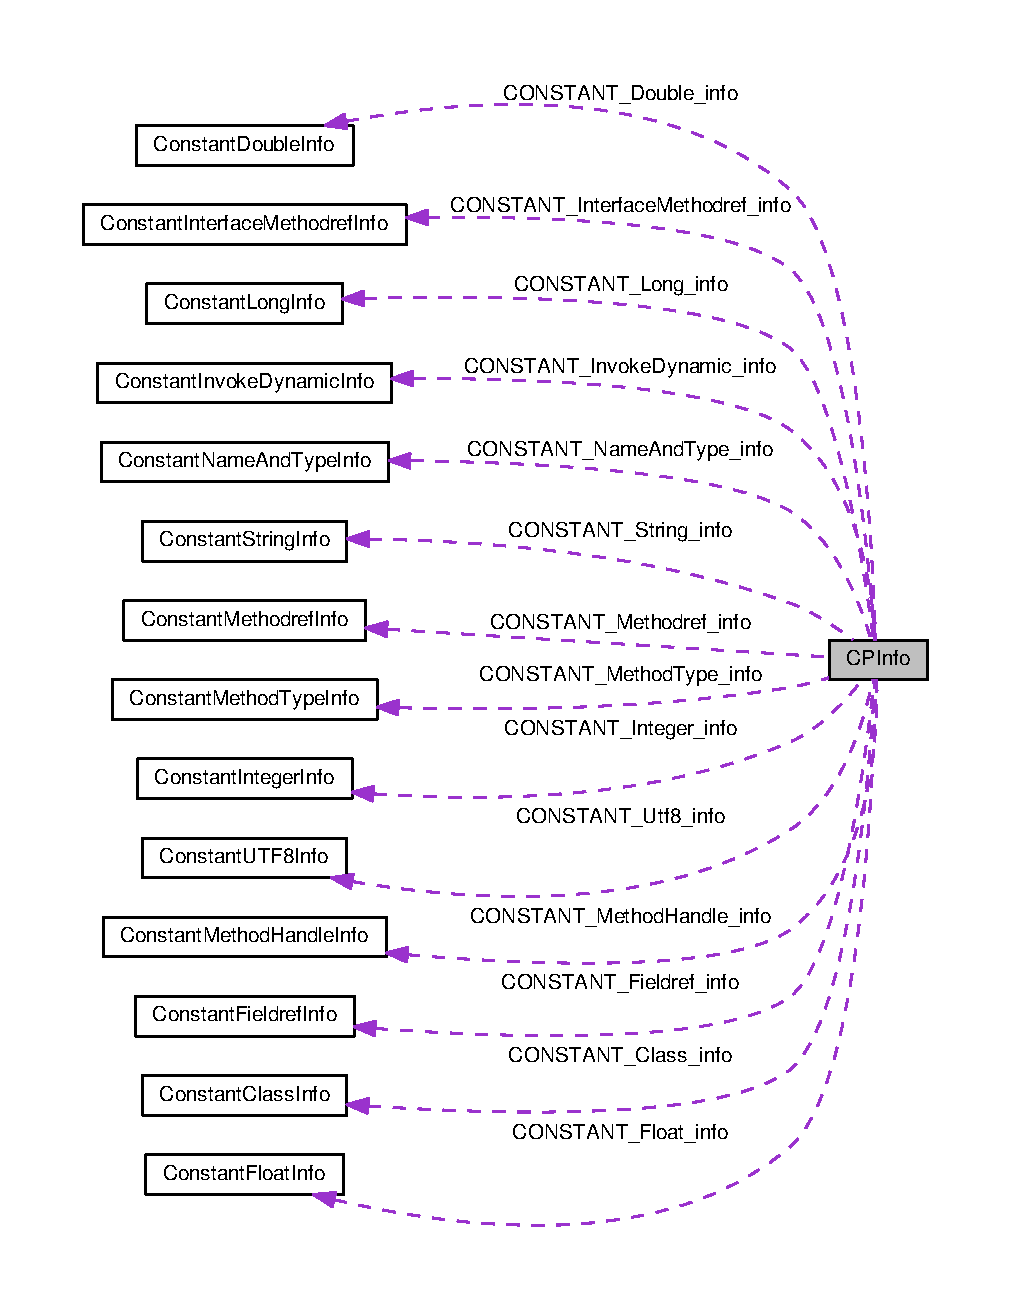
\includegraphics[width=350pt]{classCPInfo__coll__graph}
\end{center}
\end{figure}
\subsection*{Public Member Functions}
\begin{DoxyCompactItemize}
\item 
void {\bfseries read} (F\+I\+LE $\ast$fp)\hypertarget{classCPInfo_ab5fffd0d4433673806891f92edd67826}{}\label{classCPInfo_ab5fffd0d4433673806891f92edd67826}

\item 
void {\bfseries set\+Tag} (uint8\+\_\+t tag)\hypertarget{classCPInfo_aaa647d37b2b238aafcacddd027aeafe8}{}\label{classCPInfo_aaa647d37b2b238aafcacddd027aeafe8}

\item 
pair$<$ string, string $>$ {\bfseries get\+Info} (vector$<$ \hyperlink{classCPInfo}{C\+P\+Info} $\ast$ $>$ constant\+Pool)\hypertarget{classCPInfo_a331977da199d8fa56995f9de3bcb837b}{}\label{classCPInfo_a331977da199d8fa56995f9de3bcb837b}

\item 
float {\bfseries get\+Float\+Number} ()\hypertarget{classCPInfo_ab1f2f8f848bcc2fec287a243ee19ee69}{}\label{classCPInfo_ab1f2f8f848bcc2fec287a243ee19ee69}

\item 
int64\+\_\+t {\bfseries get\+Long\+Number} ()\hypertarget{classCPInfo_adec66ffc8ee4a552223e7b232a1ab5c1}{}\label{classCPInfo_adec66ffc8ee4a552223e7b232a1ab5c1}

\item 
double {\bfseries get\+Double\+Number} ()\hypertarget{classCPInfo_a65f562eac59444e0571e665f0af4bfc4}{}\label{classCPInfo_a65f562eac59444e0571e665f0af4bfc4}

\item 
uint8\+\_\+t {\bfseries get\+Tag} ()\hypertarget{classCPInfo_abea4ee7bf02eec0d9d5b86fc90f024f1}{}\label{classCPInfo_abea4ee7bf02eec0d9d5b86fc90f024f1}

\item 
\hyperlink{structConstantClassInfo}{Constant\+Class\+Info} {\bfseries get\+Class\+Info} ()\hypertarget{classCPInfo_a64411575d297ff8b50684ca5b0c93471}{}\label{classCPInfo_a64411575d297ff8b50684ca5b0c93471}

\item 
\hyperlink{structConstantFieldrefInfo}{Constant\+Fieldref\+Info} {\bfseries get\+Fieldref\+Info} ()\hypertarget{classCPInfo_ac671e911cb4b8872bd55d9a5b9f146d9}{}\label{classCPInfo_ac671e911cb4b8872bd55d9a5b9f146d9}

\item 
\hyperlink{structConstantMethodrefInfo}{Constant\+Methodref\+Info} {\bfseries get\+Methodref\+Info} ()\hypertarget{classCPInfo_ae3903d798cb11da2eb29062926a7b3f3}{}\label{classCPInfo_ae3903d798cb11da2eb29062926a7b3f3}

\item 
\hyperlink{structConstantInterfaceMethodrefInfo}{Constant\+Interface\+Methodref\+Info} {\bfseries get\+Interface\+Methodref\+Info} ()\hypertarget{classCPInfo_a42a8c3a04e943cf3e861f05078561e87}{}\label{classCPInfo_a42a8c3a04e943cf3e861f05078561e87}

\item 
\hyperlink{structConstantStringInfo}{Constant\+String\+Info} {\bfseries get\+String\+Info} ()\hypertarget{classCPInfo_adb44f35169d1e959e5c53e6a76bfcbf5}{}\label{classCPInfo_adb44f35169d1e959e5c53e6a76bfcbf5}

\item 
\hyperlink{structConstantIntegerInfo}{Constant\+Integer\+Info} {\bfseries get\+Integer\+Info} ()\hypertarget{classCPInfo_ac4ceb48810a05b9e9b7fbd2839f9e1e4}{}\label{classCPInfo_ac4ceb48810a05b9e9b7fbd2839f9e1e4}

\item 
\hyperlink{structConstantFloatInfo}{Constant\+Float\+Info} {\bfseries get\+Float\+Info} ()\hypertarget{classCPInfo_ac293e1108e36e6296e3b85576689e6cb}{}\label{classCPInfo_ac293e1108e36e6296e3b85576689e6cb}

\item 
\hyperlink{structConstantLongInfo}{Constant\+Long\+Info} {\bfseries get\+Long\+Info} ()\hypertarget{classCPInfo_ad493f187e55c0f37c2705f159a7487d9}{}\label{classCPInfo_ad493f187e55c0f37c2705f159a7487d9}

\item 
\hyperlink{structConstantDoubleInfo}{Constant\+Double\+Info} {\bfseries get\+Double\+Info} ()\hypertarget{classCPInfo_a7192445d7605e9515e3b4a5883f3b0ef}{}\label{classCPInfo_a7192445d7605e9515e3b4a5883f3b0ef}

\item 
\hyperlink{structConstantNameAndTypeInfo}{Constant\+Name\+And\+Type\+Info} {\bfseries get\+Name\+And\+Type\+Info} ()\hypertarget{classCPInfo_ae9f2c4975801d3cfc6b98a115b26fe55}{}\label{classCPInfo_ae9f2c4975801d3cfc6b98a115b26fe55}

\item 
\hyperlink{structConstantUTF8Info}{Constant\+U\+T\+F8\+Info} {\bfseries get\+U\+T\+F8\+Info} ()\hypertarget{classCPInfo_a0f40798aeacc26f85a901fc7244687a1}{}\label{classCPInfo_a0f40798aeacc26f85a901fc7244687a1}

\item 
\hyperlink{structConstantMethodHandleInfo}{Constant\+Method\+Handle\+Info} {\bfseries get\+Method\+Handle\+Info} ()\hypertarget{classCPInfo_ac8c8db8663473d3ee4074ee67f30c058}{}\label{classCPInfo_ac8c8db8663473d3ee4074ee67f30c058}

\item 
\hyperlink{structConstantMethodTypeInfo}{Constant\+Method\+Type\+Info} {\bfseries get\+Method\+Type\+Info} ()\hypertarget{classCPInfo_a35c31d16b5c67a7293b15a1f1613099a}{}\label{classCPInfo_a35c31d16b5c67a7293b15a1f1613099a}

\item 
\hyperlink{structConstantInvokeDynamicInfo}{Constant\+Invoke\+Dynamic\+Info} {\bfseries get\+Invoke\+Dynamic\+Info} ()\hypertarget{classCPInfo_a11f6eeeb39bf257a303ff640d3072bca}{}\label{classCPInfo_a11f6eeeb39bf257a303ff640d3072bca}

\end{DoxyCompactItemize}
\subsection*{Static Public Attributes}
\begin{DoxyCompactItemize}
\item 
static const uint8\+\_\+t {\bfseries C\+O\+N\+S\+T\+A\+N\+T\+\_\+\+Class} = 7\hypertarget{classCPInfo_afa2a0609b98677906efec69abd8a48e6}{}\label{classCPInfo_afa2a0609b98677906efec69abd8a48e6}

\item 
static const uint8\+\_\+t {\bfseries C\+O\+N\+S\+T\+A\+N\+T\+\_\+\+Fieldref} = 9\hypertarget{classCPInfo_a55527798317b6fd08bcbfe6052ef16a5}{}\label{classCPInfo_a55527798317b6fd08bcbfe6052ef16a5}

\item 
static const uint8\+\_\+t {\bfseries C\+O\+N\+S\+T\+A\+N\+T\+\_\+\+Methodref} = 10\hypertarget{classCPInfo_a940e4557888d69b7be96c80549fd05f8}{}\label{classCPInfo_a940e4557888d69b7be96c80549fd05f8}

\item 
static const uint8\+\_\+t {\bfseries C\+O\+N\+S\+T\+A\+N\+T\+\_\+\+Interface\+Methodref} = 11\hypertarget{classCPInfo_a3ee335fb3cd4cc6326b5a6c07027f46a}{}\label{classCPInfo_a3ee335fb3cd4cc6326b5a6c07027f46a}

\item 
static const uint8\+\_\+t {\bfseries C\+O\+N\+S\+T\+A\+N\+T\+\_\+\+String} = 8\hypertarget{classCPInfo_a5215334161f77865ffa2aae8606116e6}{}\label{classCPInfo_a5215334161f77865ffa2aae8606116e6}

\item 
static const uint8\+\_\+t {\bfseries C\+O\+N\+S\+T\+A\+N\+T\+\_\+\+Integer} = 3\hypertarget{classCPInfo_a442a6646025f8501cdf7d263e82c3912}{}\label{classCPInfo_a442a6646025f8501cdf7d263e82c3912}

\item 
static const uint8\+\_\+t {\bfseries C\+O\+N\+S\+T\+A\+N\+T\+\_\+\+Float} = 4\hypertarget{classCPInfo_aefa44ca817dd8dd7c07e951eaa472c36}{}\label{classCPInfo_aefa44ca817dd8dd7c07e951eaa472c36}

\item 
static const uint8\+\_\+t {\bfseries C\+O\+N\+S\+T\+A\+N\+T\+\_\+\+Long} = 5\hypertarget{classCPInfo_ac2edc4b97a087c8ffb458043ab38a025}{}\label{classCPInfo_ac2edc4b97a087c8ffb458043ab38a025}

\item 
static const uint8\+\_\+t {\bfseries C\+O\+N\+S\+T\+A\+N\+T\+\_\+\+Double} = 6\hypertarget{classCPInfo_a7e53dd2f4979eabea7224ec11e12f603}{}\label{classCPInfo_a7e53dd2f4979eabea7224ec11e12f603}

\item 
static const uint8\+\_\+t {\bfseries C\+O\+N\+S\+T\+A\+N\+T\+\_\+\+Name\+And\+Type} = 12\hypertarget{classCPInfo_af2407f4efc21cd1b7d92242a128804c7}{}\label{classCPInfo_af2407f4efc21cd1b7d92242a128804c7}

\item 
static const uint8\+\_\+t {\bfseries C\+O\+N\+S\+T\+A\+N\+T\+\_\+\+Utf8} = 1\hypertarget{classCPInfo_a716493735ca550f026bd00af6b709425}{}\label{classCPInfo_a716493735ca550f026bd00af6b709425}

\item 
static const uint8\+\_\+t {\bfseries C\+O\+N\+S\+T\+A\+N\+T\+\_\+\+Method\+Handle} = 15\hypertarget{classCPInfo_aa57a93a2e444d75369af492bf0885c96}{}\label{classCPInfo_aa57a93a2e444d75369af492bf0885c96}

\item 
static const uint8\+\_\+t {\bfseries C\+O\+N\+S\+T\+A\+N\+T\+\_\+\+Method\+Type} = 16\hypertarget{classCPInfo_af366bc74160698ae239cf9c8dbdd4df1}{}\label{classCPInfo_af366bc74160698ae239cf9c8dbdd4df1}

\item 
static const uint8\+\_\+t {\bfseries C\+O\+N\+S\+T\+A\+N\+T\+\_\+\+Invoke\+Dynamic} = 18\hypertarget{classCPInfo_a7930e6f14535f70bbc74fa557156e423}{}\label{classCPInfo_a7930e6f14535f70bbc74fa557156e423}

\item 
static const uint8\+\_\+t {\bfseries C\+O\+N\+S\+T\+A\+N\+T\+\_\+\+Empty} = 0\hypertarget{classCPInfo_a5a40f7d553974f74c028484d0fafde0c}{}\label{classCPInfo_a5a40f7d553974f74c028484d0fafde0c}

\end{DoxyCompactItemize}


The documentation for this class was generated from the following files\+:\begin{DoxyCompactItemize}
\item 
/home/arturhbs/\+Documentos/unb/8 semestre/\+S\+B/\+J\+V\+M/src/hpp/C\+P\+Info.\+hpp\item 
/home/arturhbs/\+Documentos/unb/8 semestre/\+S\+B/\+J\+V\+M/src/cpp/C\+P\+Info.\+cpp\end{DoxyCompactItemize}

\hypertarget{classExceptionAttribute}{}\section{Exception\+Attribute Class Reference}
\label{classExceptionAttribute}\index{Exception\+Attribute@{Exception\+Attribute}}


Classe contém number\+Of\+Exceptions e ponteiro para exception\+Index\+Table -\/ todos uint16;.  




{\ttfamily \#include $<$Attribute\+Info.\+hpp$>$}



\subsection{Detailed Description}
Classe contém number\+Of\+Exceptions e ponteiro para exception\+Index\+Table -\/ todos uint16;. 

The documentation for this class was generated from the following file\+:\begin{DoxyCompactItemize}
\item 
/home/arturhbs/\+Documentos/unb/8 semestre/\+S\+B/\+J\+V\+M/src/hpp/\hyperlink{AttributeInfo_8hpp}{Attribute\+Info.\+hpp}\end{DoxyCompactItemize}

\hypertarget{classExceptionHandler}{}\section{Exception\+Handler Class Reference}
\label{classExceptionHandler}\index{Exception\+Handler@{Exception\+Handler}}
\subsection*{Public Member Functions}
\begin{DoxyCompactItemize}
\item 
void {\bfseries read} (F\+I\+LE $\ast$fp)\hypertarget{classExceptionHandler_a9136c36e6dda68b55ad760623a4af5fc}{}\label{classExceptionHandler_a9136c36e6dda68b55ad760623a4af5fc}

\item 
uint16\+\_\+t {\bfseries get\+Start\+PC} ()\hypertarget{classExceptionHandler_a25e0e210e6638a16f2d2ae43cb9e63b2}{}\label{classExceptionHandler_a25e0e210e6638a16f2d2ae43cb9e63b2}

\item 
uint16\+\_\+t {\bfseries get\+End\+PC} ()\hypertarget{classExceptionHandler_abb77266bac3ca92769525b3a19ce07cd}{}\label{classExceptionHandler_abb77266bac3ca92769525b3a19ce07cd}

\item 
uint16\+\_\+t {\bfseries get\+Handler\+PC} ()\hypertarget{classExceptionHandler_a5288882b315614cd18ff3935d3b7deb7}{}\label{classExceptionHandler_a5288882b315614cd18ff3935d3b7deb7}

\item 
uint16\+\_\+t {\bfseries get\+Catch\+Type} ()\hypertarget{classExceptionHandler_a841a52c00770c5967c578918d3dfbde8}{}\label{classExceptionHandler_a841a52c00770c5967c578918d3dfbde8}

\end{DoxyCompactItemize}


The documentation for this class was generated from the following files\+:\begin{DoxyCompactItemize}
\item 
/home/arturhbs/\+Documentos/unb/8 semestre/\+S\+B/\+J\+V\+M/src/hpp/\hyperlink{AttributeInfo_8hpp}{Attribute\+Info.\+hpp}\item 
/home/arturhbs/\+Documentos/unb/8 semestre/\+S\+B/\+J\+V\+M/src/cpp/Attribute\+Info.\+cpp\end{DoxyCompactItemize}

\hypertarget{classExceptionsAttribute}{}\section{Exceptions\+Attribute Class Reference}
\label{classExceptionsAttribute}\index{Exceptions\+Attribute@{Exceptions\+Attribute}}
\subsection*{Classes}
\begin{DoxyCompactItemize}
\item 
class \hyperlink{classExceptionsAttribute_1_1read}{read}
\begin{DoxyCompactList}\small\item\em Método que visa armazenar os valores das exceções dos atributos. \end{DoxyCompactList}\end{DoxyCompactItemize}
\subsection*{Public Member Functions}
\begin{DoxyCompactItemize}
\item 
void {\bfseries read} (F\+I\+LE $\ast$)\hypertarget{classExceptionsAttribute_abd96393a69272508d4466fa0483c3035}{}\label{classExceptionsAttribute_abd96393a69272508d4466fa0483c3035}

\item 
uint16\+\_\+t {\bfseries get\+Number\+Of\+Exceptions} ()\hypertarget{classExceptionsAttribute_a32d7b850443b14b860a544eb7a3b5308}{}\label{classExceptionsAttribute_a32d7b850443b14b860a544eb7a3b5308}

\item 
uint16\+\_\+t $\ast$ {\bfseries get\+Exeception\+Index\+Table} ()\hypertarget{classExceptionsAttribute_a09c8f830fd0e8da6ae03ab086d28b468}{}\label{classExceptionsAttribute_a09c8f830fd0e8da6ae03ab086d28b468}

\end{DoxyCompactItemize}


The documentation for this class was generated from the following files\+:\begin{DoxyCompactItemize}
\item 
/home/arturhbs/\+Documentos/unb/8 semestre/\+S\+B/\+J\+V\+M/src/hpp/\hyperlink{AttributeInfo_8hpp}{Attribute\+Info.\+hpp}\item 
/home/arturhbs/\+Documentos/unb/8 semestre/\+S\+B/\+J\+V\+M/src/cpp/\hyperlink{AttributeInfo_8cpp}{Attribute\+Info.\+cpp}\end{DoxyCompactItemize}

\hypertarget{classExecutionEngine}{}\section{Execution\+Engine Class Reference}
\label{classExecutionEngine}\index{Execution\+Engine@{Execution\+Engine}}
\subsection*{Public Member Functions}
\begin{DoxyCompactItemize}
\item 
{\bfseries Execution\+Engine} (\hyperlink{classClassFile}{Class\+File} $\ast$, \hyperlink{classMethodArea}{Method\+Area} $\ast$, \hyperlink{classInstructionSet}{Instruction\+Set} $\ast$)\hypertarget{classExecutionEngine_a001eeecb7503b7c065a1856621331d48}{}\label{classExecutionEngine_a001eeecb7503b7c065a1856621331d48}

\item 
void {\bfseries execute} ()\hypertarget{classExecutionEngine_ae94b5187f2d6b92b1ca162b4a040235f}{}\label{classExecutionEngine_ae94b5187f2d6b92b1ca162b4a040235f}

\end{DoxyCompactItemize}


The documentation for this class was generated from the following files\+:\begin{DoxyCompactItemize}
\item 
/home/arturhbs/\+Documentos/unb/8 semestre/\+S\+B/\+J\+V\+M/src/hpp/Execution\+Engine.\+hpp\item 
/home/arturhbs/\+Documentos/unb/8 semestre/\+S\+B/\+J\+V\+M/src/cpp/Execution\+Engine.\+cpp\end{DoxyCompactItemize}

\hypertarget{classFieldInfo}{}\section{Field\+Info Class Reference}
\label{classFieldInfo}\index{Field\+Info@{Field\+Info}}


Classe que contém a estrutura de uma field;.  




{\ttfamily \#include $<$Field\+Info.\+hpp$>$}



Collaboration diagram for Field\+Info\+:\nopagebreak
\begin{figure}[H]
\begin{center}
\leavevmode
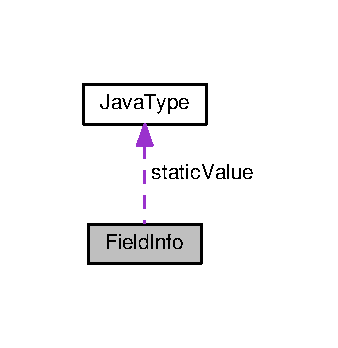
\includegraphics[width=162pt]{classFieldInfo__coll__graph}
\end{center}
\end{figure}
\subsection*{Classes}
\begin{DoxyCompactItemize}
\item 
class \hyperlink{classFieldInfo_1_1read}{read}
\begin{DoxyCompactList}\small\item\em Método com o objetivo de fazer a leitura das fields do .class. \end{DoxyCompactList}\end{DoxyCompactItemize}
\subsection*{Public Member Functions}
\begin{DoxyCompactItemize}
\item 
void {\bfseries read} (F\+I\+LE $\ast$fp, vector$<$ \hyperlink{classCPInfo}{C\+P\+Info} $\ast$ $>$ constant\+Pool)\hypertarget{classFieldInfo_ac28def66447b6ba142a7d1036b13f78f}{}\label{classFieldInfo_ac28def66447b6ba142a7d1036b13f78f}

\item 
uint16\+\_\+t {\bfseries get\+Access\+Flags} ()\hypertarget{classFieldInfo_a8f6bd79873bbf80215831234c16d03c0}{}\label{classFieldInfo_a8f6bd79873bbf80215831234c16d03c0}

\item 
uint16\+\_\+t {\bfseries get\+Name\+Index} ()\hypertarget{classFieldInfo_af0f0b36991366dabb9899799891c98e1}{}\label{classFieldInfo_af0f0b36991366dabb9899799891c98e1}

\item 
uint16\+\_\+t {\bfseries get\+Descriptor\+Index} ()\hypertarget{classFieldInfo_a48dba1ad239aa8577fbbb9b93db9d127}{}\label{classFieldInfo_a48dba1ad239aa8577fbbb9b93db9d127}

\item 
uint16\+\_\+t {\bfseries get\+Attributes\+Count} ()\hypertarget{classFieldInfo_a7a13cc4838d95f9564d7e32b8af3c452}{}\label{classFieldInfo_a7a13cc4838d95f9564d7e32b8af3c452}

\end{DoxyCompactItemize}
\subsection*{Public Attributes}
\begin{DoxyCompactItemize}
\item 
uint16\+\_\+t {\bfseries name\+Index}\hypertarget{classFieldInfo_a88ea5c29063df8933d5277e846924b1e}{}\label{classFieldInfo_a88ea5c29063df8933d5277e846924b1e}

\item 
\hyperlink{structJavaType}{Java\+Type} {\bfseries static\+Value}\hypertarget{classFieldInfo_a3dad438d44c59fc319d708c6909c1807}{}\label{classFieldInfo_a3dad438d44c59fc319d708c6909c1807}

\end{DoxyCompactItemize}
\subsection*{Static Public Attributes}
\begin{DoxyCompactItemize}
\item 
static const uint16\+\_\+t {\bfseries A\+C\+C\+\_\+\+P\+U\+B\+L\+IC} = 0x0001\hypertarget{classFieldInfo_a75f5363e21c20fc65a93fc11a9aabcd3}{}\label{classFieldInfo_a75f5363e21c20fc65a93fc11a9aabcd3}

\item 
static const uint16\+\_\+t {\bfseries A\+C\+C\+\_\+\+P\+R\+I\+V\+A\+TE} = 0x0002\hypertarget{classFieldInfo_a693cbb85341c9b61b710f56f89d56442}{}\label{classFieldInfo_a693cbb85341c9b61b710f56f89d56442}

\item 
static const uint16\+\_\+t {\bfseries A\+C\+C\+\_\+\+P\+R\+O\+T\+E\+C\+T\+ED} = 0x0004\hypertarget{classFieldInfo_ac9df52613f502a46611a670d07715d74}{}\label{classFieldInfo_ac9df52613f502a46611a670d07715d74}

\item 
static const uint16\+\_\+t {\bfseries A\+C\+C\+\_\+\+S\+T\+A\+T\+IC} = 0x0008\hypertarget{classFieldInfo_a9358cd6a36145926bedbd8718c0118c5}{}\label{classFieldInfo_a9358cd6a36145926bedbd8718c0118c5}

\item 
static const uint16\+\_\+t {\bfseries A\+C\+C\+\_\+\+F\+I\+N\+AL} = 0x0010\hypertarget{classFieldInfo_a75c707ef25ffeac2c597fb4b263d7f0c}{}\label{classFieldInfo_a75c707ef25ffeac2c597fb4b263d7f0c}

\item 
static const uint16\+\_\+t {\bfseries A\+C\+C\+\_\+\+V\+O\+L\+A\+T\+I\+LE} = 0x0040\hypertarget{classFieldInfo_abfd881c22b6614454d43b694f7917a5b}{}\label{classFieldInfo_abfd881c22b6614454d43b694f7917a5b}

\item 
static const uint16\+\_\+t {\bfseries A\+C\+C\+\_\+\+T\+R\+A\+N\+S\+I\+E\+NT} = 0x0080\hypertarget{classFieldInfo_ab92e26f398d22b736caeb5b2cad1ad31}{}\label{classFieldInfo_ab92e26f398d22b736caeb5b2cad1ad31}

\item 
static const uint16\+\_\+t {\bfseries A\+C\+C\+\_\+\+S\+Y\+N\+T\+H\+E\+T\+IC} = 0x1000\hypertarget{classFieldInfo_ab29855bcd32f7626b25f8dbcbc0e9475}{}\label{classFieldInfo_ab29855bcd32f7626b25f8dbcbc0e9475}

\item 
static const uint16\+\_\+t {\bfseries A\+C\+C\+\_\+\+E\+N\+UM} = 0x4000\hypertarget{classFieldInfo_a91b395ce72803737a57c79ba5aa3640f}{}\label{classFieldInfo_a91b395ce72803737a57c79ba5aa3640f}

\end{DoxyCompactItemize}


\subsection{Detailed Description}
Classe que contém a estrutura de uma field;. 

The documentation for this class was generated from the following files\+:\begin{DoxyCompactItemize}
\item 
/home/arturhbs/\+Documentos/unb/8 semestre/\+S\+B/\+J\+V\+M/src/hpp/\hyperlink{FieldInfo_8hpp}{Field\+Info.\+hpp}\item 
/home/arturhbs/\+Documentos/unb/8 semestre/\+S\+B/\+J\+V\+M/src/cpp/\hyperlink{FieldInfo_8cpp}{Field\+Info.\+cpp}\end{DoxyCompactItemize}

\hypertarget{classFrame}{}\section{Frame Class Reference}
\label{classFrame}\index{Frame@{Frame}}


Classe que contém todos os atributos para a criação de um frame.  




{\ttfamily \#include $<$Frame.\+hpp$>$}

\subsection*{Public Member Functions}
\begin{DoxyCompactItemize}
\item 
\hyperlink{classFrame_a422ab83c8b29489601a4bac02d4e171e}{Frame} (vector$<$ \hyperlink{classCPInfo}{C\+P\+Info} $\ast$ $>$, \hyperlink{classMethodInfo}{Method\+Info} $\ast$, stack$<$ \hyperlink{classFrame}{Frame} $>$ $\ast$)
\begin{DoxyCompactList}\small\item\em Construtor. \end{DoxyCompactList}\item 
uint8\+\_\+t $\ast$ {\bfseries get\+Code} ()\hypertarget{classFrame_aac40e0ebfeb7b3298b59c37a7f4e3006}{}\label{classFrame_aac40e0ebfeb7b3298b59c37a7f4e3006}

\item 
uint32\+\_\+t {\bfseries get\+Code\+Length} ()\hypertarget{classFrame_a9233523486da4fa4ac786883f519fe17}{}\label{classFrame_a9233523486da4fa4ac786883f519fe17}

\end{DoxyCompactItemize}
\subsection*{Public Attributes}
\begin{DoxyCompactItemize}
\item 
vector$<$ \hyperlink{classCPInfo}{C\+P\+Info} $\ast$ $>$ {\bfseries constant\+Pool}\hypertarget{classFrame_a7f1b0dca3dccb5cf3c92c35f1d0f2ef3}{}\label{classFrame_a7f1b0dca3dccb5cf3c92c35f1d0f2ef3}

\item 
stack$<$ \hyperlink{structJavaType}{Java\+Type} $>$ {\bfseries operand\+Stack}\hypertarget{classFrame_a5ed7f6e3ef7c99846894cb09597a3b3f}{}\label{classFrame_a5ed7f6e3ef7c99846894cb09597a3b3f}

\item 
vector$<$ \hyperlink{structJavaType}{Java\+Type} $>$ {\bfseries local\+Variables}\hypertarget{classFrame_af2f6d1ea56afb31babe6b10d3718bb65}{}\label{classFrame_af2f6d1ea56afb31babe6b10d3718bb65}

\item 
stack$<$ \hyperlink{classFrame}{Frame} $>$ $\ast$ {\bfseries jvm\+Stack}\hypertarget{classFrame_a985706d77698649f468e37414612a9a8}{}\label{classFrame_a985706d77698649f468e37414612a9a8}

\item 
uint32\+\_\+t {\bfseries local\+PC}\hypertarget{classFrame_a1e4cb428fe4e3008590cb9bebfdca2a1}{}\label{classFrame_a1e4cb428fe4e3008590cb9bebfdca2a1}

\end{DoxyCompactItemize}


\subsection{Detailed Description}
Classe que contém todos os atributos para a criação de um frame. 

\subsection{Constructor \& Destructor Documentation}
\index{Frame@{Frame}!Frame@{Frame}}
\index{Frame@{Frame}!Frame@{Frame}}
\subsubsection[{\texorpdfstring{Frame(vector$<$ C\+P\+Info $\ast$ $>$, Method\+Info $\ast$, stack$<$ Frame $>$ $\ast$)}{Frame(vector< CPInfo * >, MethodInfo *, stack< Frame > *)}}]{\setlength{\rightskip}{0pt plus 5cm}Frame\+::\+Frame (
\begin{DoxyParamCaption}
\item[{vector$<$ {\bf C\+P\+Info} $\ast$ $>$}]{constant\+Pool, }
\item[{{\bf Method\+Info} $\ast$}]{method, }
\item[{stack$<$ {\bf Frame} $>$ $\ast$}]{jvm\+Stack}
\end{DoxyParamCaption}
)}\hypertarget{classFrame_a422ab83c8b29489601a4bac02d4e171e}{}\label{classFrame_a422ab83c8b29489601a4bac02d4e171e}


Construtor. 


\begin{DoxyParams}{Parameters}
{\em constant\+Pool} & do tipo \hyperlink{classCPInfo}{C\+P\+Info} \\
\hline
{\em method} & do tipo \hyperlink{classMethodInfo}{Method\+Info} \\
\hline
{\em jvm\+Stack} & pilha do tipo \hyperlink{classFrame}{Frame} \\
\hline
\end{DoxyParams}
\begin{DoxyReturn}{Returns}

\end{DoxyReturn}


The documentation for this class was generated from the following files\+:\begin{DoxyCompactItemize}
\item 
/home/arturhbs/\+Documentos/unb/8 semestre/\+S\+B/\+J\+V\+M/src/hpp/\hyperlink{Frame_8hpp}{Frame.\+hpp}\item 
/home/arturhbs/\+Documentos/unb/8 semestre/\+S\+B/\+J\+V\+M/src/cpp/\hyperlink{Frame_8cpp}{Frame.\+cpp}\end{DoxyCompactItemize}

\hypertarget{classHeap}{}\section{Heap Class Reference}
\label{classHeap}\index{Heap@{Heap}}


The documentation for this class was generated from the following file\+:\begin{DoxyCompactItemize}
\item 
/home/arturhbs/\+Documentos/unb/8 semestre/\+S\+B/\+J\+V\+M/src/hpp/Heap.\+hpp\end{DoxyCompactItemize}

\hypertarget{classInnerClassesAttribute}{}\section{Inner\+Classes\+Attribute Class Reference}
\label{classInnerClassesAttribute}\index{Inner\+Classes\+Attribute@{Inner\+Classes\+Attribute}}
\subsection*{Public Member Functions}
\begin{DoxyCompactItemize}
\item 
void {\bfseries read} (F\+I\+LE $\ast$)\hypertarget{classInnerClassesAttribute_ae43a7123a6838f72aebd1b0a829bfb3d}{}\label{classInnerClassesAttribute_ae43a7123a6838f72aebd1b0a829bfb3d}

\item 
uint16\+\_\+t {\bfseries get\+Number\+Of\+Classes} ()\hypertarget{classInnerClassesAttribute_ad22800b6d8b252ee045c438258549570}{}\label{classInnerClassesAttribute_ad22800b6d8b252ee045c438258549570}

\item 
\hyperlink{classClassInfo}{Class\+Info} $\ast$ {\bfseries get\+Classes} ()\hypertarget{classInnerClassesAttribute_a9e5d2a9b9304e72f532ef6033dac8eea}{}\label{classInnerClassesAttribute_a9e5d2a9b9304e72f532ef6033dac8eea}

\end{DoxyCompactItemize}


The documentation for this class was generated from the following files\+:\begin{DoxyCompactItemize}
\item 
/home/arturhbs/\+Documentos/unb/8 semestre/\+S\+B/\+J\+V\+M/src/hpp/\hyperlink{AttributeInfo_8hpp}{Attribute\+Info.\+hpp}\item 
/home/arturhbs/\+Documentos/unb/8 semestre/\+S\+B/\+J\+V\+M/src/cpp/Attribute\+Info.\+cpp\end{DoxyCompactItemize}

\hypertarget{classInstruction}{}\section{Instruction Class Reference}
\label{classInstruction}\index{Instruction@{Instruction}}


Classe que contém a estrutura de uma instrução a ser executada pelo interpretador;.  




{\ttfamily \#include $<$Instruction.\+hpp$>$}



Collaboration diagram for Instruction\+:
\nopagebreak
\begin{figure}[H]
\begin{center}
\leavevmode
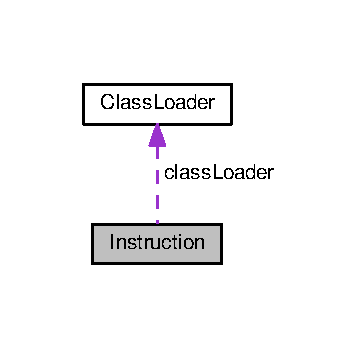
\includegraphics[width=172pt]{classInstruction__coll__graph}
\end{center}
\end{figure}
\subsection*{Public Member Functions}
\begin{DoxyCompactItemize}
\item 
{\bfseries Instruction} (string, uint32\+\_\+t, uint32\+\_\+t($\ast$)(\hyperlink{classFrame}{Frame} $\ast$))\hypertarget{classInstruction_a796b0697656d6d1230d94f942680245b}{}\label{classInstruction_a796b0697656d6d1230d94f942680245b}

\item 
void {\bfseries set\+Mnemonic} (string)\hypertarget{classInstruction_a507efd4e2f184c09f4349b682479bfb5}{}\label{classInstruction_a507efd4e2f184c09f4349b682479bfb5}

\item 
void {\bfseries set\+Bytes\+Count} (uint32\+\_\+t)\hypertarget{classInstruction_a963419f34dc60eba3f5e5d8aa86da6f2}{}\label{classInstruction_a963419f34dc60eba3f5e5d8aa86da6f2}

\item 
string {\bfseries get\+Mnemonic} ()\hypertarget{classInstruction_a467cd8f7f8f8d22c9d3d26c9dbbb6b97}{}\label{classInstruction_a467cd8f7f8f8d22c9d3d26c9dbbb6b97}

\item 
uint32\+\_\+t {\bfseries get\+Bytes\+Count} ()\hypertarget{classInstruction_a0cc76fd49fa6bc6f7ec395484fa18cb3}{}\label{classInstruction_a0cc76fd49fa6bc6f7ec395484fa18cb3}

\end{DoxyCompactItemize}
\subsection*{Static Public Member Functions}
\begin{DoxyCompactItemize}
\item 
static void {\bfseries set\+Class\+Loader} (\hyperlink{classClassLoader}{Class\+Loader} $\ast$)\hypertarget{classInstruction_ae43b3c062c5fa3d20e8d0fdb588f440e}{}\label{classInstruction_ae43b3c062c5fa3d20e8d0fdb588f440e}

\item 
static map$<$ string, \hyperlink{structJavaType}{Java\+Type} $>$ $\ast$ {\bfseries initialize\+Fields} (\hyperlink{classClassFile}{Class\+File} $\ast$)\hypertarget{classInstruction_a65ca043d7540ccb9cc9dbf014bb324e8}{}\label{classInstruction_a65ca043d7540ccb9cc9dbf014bb324e8}

\item 
static vector$<$ \hyperlink{structJavaType}{Java\+Type} $>$ $\ast$ {\bfseries build\+Multi\+Anew\+Array} (vector$<$ int $>$, int, char)\hypertarget{classInstruction_a8e4b8b07ca5bb5e4fe7f20067b82cb5b}{}\label{classInstruction_a8e4b8b07ca5bb5e4fe7f20067b82cb5b}

\item 
static \hyperlink{classClassFile}{Class\+File} $\ast$ {\bfseries resolve\+Class} (string)\hypertarget{classInstruction_a8b0bc39eafe9e944256384e9e6819242}{}\label{classInstruction_a8b0bc39eafe9e944256384e9e6819242}

\item 
static \hyperlink{classFieldInfo}{Field\+Info} $\ast$ {\bfseries resolve\+Field} (\hyperlink{classClassFile}{Class\+File} $\ast$, string, string)\hypertarget{classInstruction_a0638fefe757efeaf7b6f2681f228899e}{}\label{classInstruction_a0638fefe757efeaf7b6f2681f228899e}

\item 
static uint32\+\_\+t {\bfseries nop\+Function} (\hyperlink{classFrame}{Frame} $\ast$)\hypertarget{classInstruction_a6f0c78ca85ceae1afe891aaf65d20add}{}\label{classInstruction_a6f0c78ca85ceae1afe891aaf65d20add}

\item 
static uint32\+\_\+t {\bfseries aconst\+\_\+null\+Function} (\hyperlink{classFrame}{Frame} $\ast$)\hypertarget{classInstruction_a6c043292e2f8252c1bf6f4f207ad411b}{}\label{classInstruction_a6c043292e2f8252c1bf6f4f207ad411b}

\item 
static uint32\+\_\+t {\bfseries iconst\+\_\+m1\+Function} (\hyperlink{classFrame}{Frame} $\ast$)\hypertarget{classInstruction_ae655faaa7e07e17ee09baf5c1994b5b7}{}\label{classInstruction_ae655faaa7e07e17ee09baf5c1994b5b7}

\item 
static uint32\+\_\+t {\bfseries iconst\+\_\+0\+Function} (\hyperlink{classFrame}{Frame} $\ast$)\hypertarget{classInstruction_aea29a9c4bc3073454794c1e298ac9b8d}{}\label{classInstruction_aea29a9c4bc3073454794c1e298ac9b8d}

\item 
static uint32\+\_\+t {\bfseries iconst\+\_\+1\+Function} (\hyperlink{classFrame}{Frame} $\ast$)\hypertarget{classInstruction_ac9ba4fa3f80679b580e27e54fcd43332}{}\label{classInstruction_ac9ba4fa3f80679b580e27e54fcd43332}

\item 
static uint32\+\_\+t {\bfseries iconst\+\_\+2\+Function} (\hyperlink{classFrame}{Frame} $\ast$)\hypertarget{classInstruction_a8f98b5a0b5508b85bf8b4436fc85439a}{}\label{classInstruction_a8f98b5a0b5508b85bf8b4436fc85439a}

\item 
static uint32\+\_\+t {\bfseries iconst\+\_\+3\+Function} (\hyperlink{classFrame}{Frame} $\ast$)\hypertarget{classInstruction_a084cecaa9593a77651b9c8f5375fe87a}{}\label{classInstruction_a084cecaa9593a77651b9c8f5375fe87a}

\item 
static uint32\+\_\+t {\bfseries iconst\+\_\+4\+Function} (\hyperlink{classFrame}{Frame} $\ast$)\hypertarget{classInstruction_a915b20a8ea70a73af435a10fdc4d1c4f}{}\label{classInstruction_a915b20a8ea70a73af435a10fdc4d1c4f}

\item 
static uint32\+\_\+t {\bfseries iconst\+\_\+5\+Function} (\hyperlink{classFrame}{Frame} $\ast$)\hypertarget{classInstruction_a884daf4445b195d75eacbc22265ea69b}{}\label{classInstruction_a884daf4445b195d75eacbc22265ea69b}

\item 
static uint32\+\_\+t {\bfseries lconst\+\_\+0\+Function} (\hyperlink{classFrame}{Frame} $\ast$)\hypertarget{classInstruction_acce02061398a5f44654238430119ff22}{}\label{classInstruction_acce02061398a5f44654238430119ff22}

\item 
static uint32\+\_\+t {\bfseries lconst\+\_\+1\+Function} (\hyperlink{classFrame}{Frame} $\ast$)\hypertarget{classInstruction_ae6c48360c78c8d6e252070a9f9c4ac79}{}\label{classInstruction_ae6c48360c78c8d6e252070a9f9c4ac79}

\item 
static uint32\+\_\+t {\bfseries fconst\+\_\+0\+Function} (\hyperlink{classFrame}{Frame} $\ast$)\hypertarget{classInstruction_a80a4bd1f9903bba1bd8118711d75c444}{}\label{classInstruction_a80a4bd1f9903bba1bd8118711d75c444}

\item 
static uint32\+\_\+t {\bfseries fconst\+\_\+1\+Function} (\hyperlink{classFrame}{Frame} $\ast$)\hypertarget{classInstruction_a35e282a2ba528d11562f704d06b2a267}{}\label{classInstruction_a35e282a2ba528d11562f704d06b2a267}

\item 
static uint32\+\_\+t {\bfseries fconst\+\_\+2\+Function} (\hyperlink{classFrame}{Frame} $\ast$)\hypertarget{classInstruction_ad140a6ddc9c5722bbc4d876673c3881a}{}\label{classInstruction_ad140a6ddc9c5722bbc4d876673c3881a}

\item 
static uint32\+\_\+t {\bfseries dconst\+\_\+0\+Function} (\hyperlink{classFrame}{Frame} $\ast$)\hypertarget{classInstruction_a65be48b87cb978d14a76722ed3727487}{}\label{classInstruction_a65be48b87cb978d14a76722ed3727487}

\item 
static uint32\+\_\+t {\bfseries dconst\+\_\+1\+Function} (\hyperlink{classFrame}{Frame} $\ast$)\hypertarget{classInstruction_aa7daf88bc1faf1fa465c62e78d0e3c2b}{}\label{classInstruction_aa7daf88bc1faf1fa465c62e78d0e3c2b}

\item 
static uint32\+\_\+t {\bfseries bipush\+Function} (\hyperlink{classFrame}{Frame} $\ast$)\hypertarget{classInstruction_abe0b8b1c00bbff6e6f685b63a521545f}{}\label{classInstruction_abe0b8b1c00bbff6e6f685b63a521545f}

\item 
static uint32\+\_\+t {\bfseries sipush\+Function} (\hyperlink{classFrame}{Frame} $\ast$)\hypertarget{classInstruction_a56b869507cdc4592f3a9f70abb05addf}{}\label{classInstruction_a56b869507cdc4592f3a9f70abb05addf}

\item 
static uint32\+\_\+t {\bfseries ldc\+Function} (\hyperlink{classFrame}{Frame} $\ast$)\hypertarget{classInstruction_a12faac99a733e2847cf22aaacb33b005}{}\label{classInstruction_a12faac99a733e2847cf22aaacb33b005}

\item 
static uint32\+\_\+t {\bfseries ldc\+\_\+w\+Function} (\hyperlink{classFrame}{Frame} $\ast$)\hypertarget{classInstruction_a00c074a19f363fc670654e554aef3f92}{}\label{classInstruction_a00c074a19f363fc670654e554aef3f92}

\item 
static uint32\+\_\+t {\bfseries ldc2\+\_\+w\+Function} (\hyperlink{classFrame}{Frame} $\ast$)\hypertarget{classInstruction_a7e1f2735b08557ccbb9438fced9af5d2}{}\label{classInstruction_a7e1f2735b08557ccbb9438fced9af5d2}

\item 
static uint32\+\_\+t {\bfseries iload\+Function} (\hyperlink{classFrame}{Frame} $\ast$)\hypertarget{classInstruction_ac49a430c05b1edfe6cff774d9f967828}{}\label{classInstruction_ac49a430c05b1edfe6cff774d9f967828}

\item 
static uint32\+\_\+t {\bfseries lload\+Function} (\hyperlink{classFrame}{Frame} $\ast$)\hypertarget{classInstruction_a81a0fc970bfeebe8391e05891c6c26a0}{}\label{classInstruction_a81a0fc970bfeebe8391e05891c6c26a0}

\item 
static uint32\+\_\+t {\bfseries fload\+Function} (\hyperlink{classFrame}{Frame} $\ast$)\hypertarget{classInstruction_a3c63384ee0a0b0af0764e3a61672401e}{}\label{classInstruction_a3c63384ee0a0b0af0764e3a61672401e}

\item 
static uint32\+\_\+t {\bfseries dload\+Function} (\hyperlink{classFrame}{Frame} $\ast$)\hypertarget{classInstruction_a32bfa514a38d8d1ac933388cd91295f2}{}\label{classInstruction_a32bfa514a38d8d1ac933388cd91295f2}

\item 
static uint32\+\_\+t {\bfseries aload\+Function} (\hyperlink{classFrame}{Frame} $\ast$)\hypertarget{classInstruction_a27cf8204f7c1c1b4f9e103b0a8a61376}{}\label{classInstruction_a27cf8204f7c1c1b4f9e103b0a8a61376}

\item 
static uint32\+\_\+t {\bfseries iload\+\_\+0\+Function} (\hyperlink{classFrame}{Frame} $\ast$)\hypertarget{classInstruction_a949bf6ed1b98cdace0d0dfee6d0ccf12}{}\label{classInstruction_a949bf6ed1b98cdace0d0dfee6d0ccf12}

\item 
static uint32\+\_\+t {\bfseries iload\+\_\+1\+Function} (\hyperlink{classFrame}{Frame} $\ast$)\hypertarget{classInstruction_ae377f538a102555828609efbdf8dbcbf}{}\label{classInstruction_ae377f538a102555828609efbdf8dbcbf}

\item 
static uint32\+\_\+t {\bfseries iload\+\_\+2\+Function} (\hyperlink{classFrame}{Frame} $\ast$)\hypertarget{classInstruction_a93d395cd6b6894b6df1bf73c60580dfc}{}\label{classInstruction_a93d395cd6b6894b6df1bf73c60580dfc}

\item 
static uint32\+\_\+t {\bfseries iload\+\_\+3\+Function} (\hyperlink{classFrame}{Frame} $\ast$)\hypertarget{classInstruction_a6d58dfc3679b9e52121f179f7563996b}{}\label{classInstruction_a6d58dfc3679b9e52121f179f7563996b}

\item 
static uint32\+\_\+t {\bfseries lload\+\_\+0\+Function} (\hyperlink{classFrame}{Frame} $\ast$)\hypertarget{classInstruction_a0a6e96c7994e50ff6740e417b21298ca}{}\label{classInstruction_a0a6e96c7994e50ff6740e417b21298ca}

\item 
static uint32\+\_\+t {\bfseries lload\+\_\+1\+Function} (\hyperlink{classFrame}{Frame} $\ast$)\hypertarget{classInstruction_a89f36c5a5a394d04fc105dc1c31aa5af}{}\label{classInstruction_a89f36c5a5a394d04fc105dc1c31aa5af}

\item 
static uint32\+\_\+t {\bfseries lload\+\_\+2\+Function} (\hyperlink{classFrame}{Frame} $\ast$)\hypertarget{classInstruction_a174fd405703d7259a2d8ed28e5aa6a36}{}\label{classInstruction_a174fd405703d7259a2d8ed28e5aa6a36}

\item 
static uint32\+\_\+t {\bfseries lload\+\_\+3\+Function} (\hyperlink{classFrame}{Frame} $\ast$)\hypertarget{classInstruction_a9716ecdc90087a8ba0a88e93d7e23fdc}{}\label{classInstruction_a9716ecdc90087a8ba0a88e93d7e23fdc}

\item 
static uint32\+\_\+t {\bfseries fload\+\_\+0\+Function} (\hyperlink{classFrame}{Frame} $\ast$)\hypertarget{classInstruction_aa7dbc98447c0be1be87f805c2a10f371}{}\label{classInstruction_aa7dbc98447c0be1be87f805c2a10f371}

\item 
static uint32\+\_\+t {\bfseries fload\+\_\+1\+Function} (\hyperlink{classFrame}{Frame} $\ast$)\hypertarget{classInstruction_a7cb55593657d432db8c62a82d663a8d6}{}\label{classInstruction_a7cb55593657d432db8c62a82d663a8d6}

\item 
static uint32\+\_\+t {\bfseries fload\+\_\+2\+Function} (\hyperlink{classFrame}{Frame} $\ast$)\hypertarget{classInstruction_aca2aab1eae22c61877124f5c5e7381b3}{}\label{classInstruction_aca2aab1eae22c61877124f5c5e7381b3}

\item 
static uint32\+\_\+t {\bfseries fload\+\_\+3\+Function} (\hyperlink{classFrame}{Frame} $\ast$)\hypertarget{classInstruction_a7ef95cdb7804f18dd78db5ac0b084944}{}\label{classInstruction_a7ef95cdb7804f18dd78db5ac0b084944}

\item 
static uint32\+\_\+t {\bfseries dload\+\_\+0\+Function} (\hyperlink{classFrame}{Frame} $\ast$)\hypertarget{classInstruction_a136a8418463be8dd22ab241dee71b21b}{}\label{classInstruction_a136a8418463be8dd22ab241dee71b21b}

\item 
static uint32\+\_\+t {\bfseries dload\+\_\+1\+Function} (\hyperlink{classFrame}{Frame} $\ast$)\hypertarget{classInstruction_a49b06a94a1259a2ad2113df05d6b61dc}{}\label{classInstruction_a49b06a94a1259a2ad2113df05d6b61dc}

\item 
static uint32\+\_\+t {\bfseries dload\+\_\+2\+Function} (\hyperlink{classFrame}{Frame} $\ast$)\hypertarget{classInstruction_aa2880575212d8c904ff600e7e2bd8c6c}{}\label{classInstruction_aa2880575212d8c904ff600e7e2bd8c6c}

\item 
static uint32\+\_\+t {\bfseries dload\+\_\+3\+Function} (\hyperlink{classFrame}{Frame} $\ast$)\hypertarget{classInstruction_ab3b15a82420744850f05fc5dc2344861}{}\label{classInstruction_ab3b15a82420744850f05fc5dc2344861}

\item 
static uint32\+\_\+t {\bfseries aload\+\_\+0\+Function} (\hyperlink{classFrame}{Frame} $\ast$)\hypertarget{classInstruction_afebfe7875bc4c9da55a08f2fbd37ccc8}{}\label{classInstruction_afebfe7875bc4c9da55a08f2fbd37ccc8}

\item 
static uint32\+\_\+t {\bfseries aload\+\_\+1\+Function} (\hyperlink{classFrame}{Frame} $\ast$)\hypertarget{classInstruction_ad726348f71f64d3412666d8f0850152c}{}\label{classInstruction_ad726348f71f64d3412666d8f0850152c}

\item 
static uint32\+\_\+t {\bfseries aload\+\_\+2\+Function} (\hyperlink{classFrame}{Frame} $\ast$)\hypertarget{classInstruction_a64a990cb129159c216a889546dc1a66c}{}\label{classInstruction_a64a990cb129159c216a889546dc1a66c}

\item 
static uint32\+\_\+t {\bfseries aload\+\_\+3\+Function} (\hyperlink{classFrame}{Frame} $\ast$)\hypertarget{classInstruction_a844a1ff21cb214c46a422d08b2fc75f3}{}\label{classInstruction_a844a1ff21cb214c46a422d08b2fc75f3}

\item 
static uint32\+\_\+t {\bfseries iaload\+Function} (\hyperlink{classFrame}{Frame} $\ast$)\hypertarget{classInstruction_a27e1a1fd58c8834b5e806309f37cd30b}{}\label{classInstruction_a27e1a1fd58c8834b5e806309f37cd30b}

\item 
static uint32\+\_\+t {\bfseries laload\+Function} (\hyperlink{classFrame}{Frame} $\ast$)\hypertarget{classInstruction_a10912858a3914e0704c35801a16a6635}{}\label{classInstruction_a10912858a3914e0704c35801a16a6635}

\item 
static uint32\+\_\+t {\bfseries faload\+Function} (\hyperlink{classFrame}{Frame} $\ast$)\hypertarget{classInstruction_abf5a06c62052a59a967f0699ba082a56}{}\label{classInstruction_abf5a06c62052a59a967f0699ba082a56}

\item 
static uint32\+\_\+t {\bfseries daload\+Function} (\hyperlink{classFrame}{Frame} $\ast$)\hypertarget{classInstruction_a4a08ea20e145e4072f1b2de66aca205b}{}\label{classInstruction_a4a08ea20e145e4072f1b2de66aca205b}

\item 
static uint32\+\_\+t {\bfseries aaload\+Function} (\hyperlink{classFrame}{Frame} $\ast$)\hypertarget{classInstruction_a6801f5d7f403d9c4970a5440ba8e9dac}{}\label{classInstruction_a6801f5d7f403d9c4970a5440ba8e9dac}

\item 
static uint32\+\_\+t {\bfseries baload\+Function} (\hyperlink{classFrame}{Frame} $\ast$)\hypertarget{classInstruction_a484c020aca89980472184b70bdafa7e1}{}\label{classInstruction_a484c020aca89980472184b70bdafa7e1}

\item 
static uint32\+\_\+t {\bfseries caload\+Function} (\hyperlink{classFrame}{Frame} $\ast$)\hypertarget{classInstruction_a5c456ad11a23c88468d8184c364c3506}{}\label{classInstruction_a5c456ad11a23c88468d8184c364c3506}

\item 
static uint32\+\_\+t {\bfseries saload\+Function} (\hyperlink{classFrame}{Frame} $\ast$)\hypertarget{classInstruction_a886cd51264c0acd9d99baee8969a3728}{}\label{classInstruction_a886cd51264c0acd9d99baee8969a3728}

\item 
static uint32\+\_\+t {\bfseries istore\+Function} (\hyperlink{classFrame}{Frame} $\ast$)\hypertarget{classInstruction_a59e1ba8ddd0a1797884b75c48935734d}{}\label{classInstruction_a59e1ba8ddd0a1797884b75c48935734d}

\item 
static uint32\+\_\+t {\bfseries lstore\+Function} (\hyperlink{classFrame}{Frame} $\ast$)\hypertarget{classInstruction_a51889334cb02667687e4fa75d358c034}{}\label{classInstruction_a51889334cb02667687e4fa75d358c034}

\item 
static uint32\+\_\+t {\bfseries fstore\+Function} (\hyperlink{classFrame}{Frame} $\ast$)\hypertarget{classInstruction_aea1cc3a1ea56553fbda914df045724f6}{}\label{classInstruction_aea1cc3a1ea56553fbda914df045724f6}

\item 
static uint32\+\_\+t {\bfseries dstore\+Function} (\hyperlink{classFrame}{Frame} $\ast$)\hypertarget{classInstruction_a616031221196dc855a197d040eda77ef}{}\label{classInstruction_a616031221196dc855a197d040eda77ef}

\item 
static uint32\+\_\+t {\bfseries astore\+Function} (\hyperlink{classFrame}{Frame} $\ast$)\hypertarget{classInstruction_a17640bb433ab7e94d7608c3de12dfdc7}{}\label{classInstruction_a17640bb433ab7e94d7608c3de12dfdc7}

\item 
static uint32\+\_\+t {\bfseries istore\+\_\+0\+Function} (\hyperlink{classFrame}{Frame} $\ast$)\hypertarget{classInstruction_a57e45b6047cfcfb00bdef70f778d4a03}{}\label{classInstruction_a57e45b6047cfcfb00bdef70f778d4a03}

\item 
static uint32\+\_\+t {\bfseries istore\+\_\+1\+Function} (\hyperlink{classFrame}{Frame} $\ast$)\hypertarget{classInstruction_a59d58c02463de3b0bfffdf02aaa9f2cb}{}\label{classInstruction_a59d58c02463de3b0bfffdf02aaa9f2cb}

\item 
static uint32\+\_\+t {\bfseries istore\+\_\+2\+Function} (\hyperlink{classFrame}{Frame} $\ast$)\hypertarget{classInstruction_a8a1515ffe227235d85bbac080c7c2055}{}\label{classInstruction_a8a1515ffe227235d85bbac080c7c2055}

\item 
static uint32\+\_\+t {\bfseries istore\+\_\+3\+Function} (\hyperlink{classFrame}{Frame} $\ast$)\hypertarget{classInstruction_a90afad2c2a31af23228cff703b1ef7e8}{}\label{classInstruction_a90afad2c2a31af23228cff703b1ef7e8}

\item 
static uint32\+\_\+t {\bfseries lstore\+\_\+0\+Function} (\hyperlink{classFrame}{Frame} $\ast$)\hypertarget{classInstruction_ae350cb40e9e8d328891f1a438c732f49}{}\label{classInstruction_ae350cb40e9e8d328891f1a438c732f49}

\item 
static uint32\+\_\+t {\bfseries lstore\+\_\+1\+Function} (\hyperlink{classFrame}{Frame} $\ast$)\hypertarget{classInstruction_a931bb47208f7277fed3b05478e49ec3c}{}\label{classInstruction_a931bb47208f7277fed3b05478e49ec3c}

\item 
static uint32\+\_\+t {\bfseries lstore\+\_\+2\+Function} (\hyperlink{classFrame}{Frame} $\ast$)\hypertarget{classInstruction_a1990d5d8ff7457e7f92678b0c1fff855}{}\label{classInstruction_a1990d5d8ff7457e7f92678b0c1fff855}

\item 
static uint32\+\_\+t {\bfseries lstore\+\_\+3\+Function} (\hyperlink{classFrame}{Frame} $\ast$)\hypertarget{classInstruction_a01a6cd69b5e7838160fea094f60805f2}{}\label{classInstruction_a01a6cd69b5e7838160fea094f60805f2}

\item 
static uint32\+\_\+t {\bfseries fstore\+\_\+0\+Function} (\hyperlink{classFrame}{Frame} $\ast$)\hypertarget{classInstruction_a46639c2eef051acbbaf6546ef091ddca}{}\label{classInstruction_a46639c2eef051acbbaf6546ef091ddca}

\item 
static uint32\+\_\+t {\bfseries fstore\+\_\+1\+Function} (\hyperlink{classFrame}{Frame} $\ast$)\hypertarget{classInstruction_acc3b0f3a649352eb4d654a48092a97bf}{}\label{classInstruction_acc3b0f3a649352eb4d654a48092a97bf}

\item 
static uint32\+\_\+t {\bfseries fstore\+\_\+2\+Function} (\hyperlink{classFrame}{Frame} $\ast$)\hypertarget{classInstruction_a373ffebd2ede054e5535a182c4a46937}{}\label{classInstruction_a373ffebd2ede054e5535a182c4a46937}

\item 
static uint32\+\_\+t {\bfseries fstore\+\_\+3\+Function} (\hyperlink{classFrame}{Frame} $\ast$)\hypertarget{classInstruction_a8c496adfee102f7ee29646abc91ffd0c}{}\label{classInstruction_a8c496adfee102f7ee29646abc91ffd0c}

\item 
static uint32\+\_\+t {\bfseries dstore\+\_\+0\+Function} (\hyperlink{classFrame}{Frame} $\ast$)\hypertarget{classInstruction_acb952a3098170b2a3b9ad9115a434f29}{}\label{classInstruction_acb952a3098170b2a3b9ad9115a434f29}

\item 
static uint32\+\_\+t {\bfseries dstore\+\_\+1\+Function} (\hyperlink{classFrame}{Frame} $\ast$)\hypertarget{classInstruction_aaeecc1f448ec4970f5c16bd64acd76cb}{}\label{classInstruction_aaeecc1f448ec4970f5c16bd64acd76cb}

\item 
static uint32\+\_\+t {\bfseries dstore\+\_\+2\+Function} (\hyperlink{classFrame}{Frame} $\ast$)\hypertarget{classInstruction_a20a195cfccb82328f06d51302c9ce8f3}{}\label{classInstruction_a20a195cfccb82328f06d51302c9ce8f3}

\item 
static uint32\+\_\+t {\bfseries dstore\+\_\+3\+Function} (\hyperlink{classFrame}{Frame} $\ast$)\hypertarget{classInstruction_a362991c1b52a478c967847f4ea66baa1}{}\label{classInstruction_a362991c1b52a478c967847f4ea66baa1}

\item 
static uint32\+\_\+t {\bfseries astore\+\_\+0\+Function} (\hyperlink{classFrame}{Frame} $\ast$)\hypertarget{classInstruction_ae16a85e2f865e513803e8566f565caf9}{}\label{classInstruction_ae16a85e2f865e513803e8566f565caf9}

\item 
static uint32\+\_\+t {\bfseries astore\+\_\+1\+Function} (\hyperlink{classFrame}{Frame} $\ast$)\hypertarget{classInstruction_a39a042a26ca7258168413531caf1ec6a}{}\label{classInstruction_a39a042a26ca7258168413531caf1ec6a}

\item 
static uint32\+\_\+t {\bfseries astore\+\_\+2\+Function} (\hyperlink{classFrame}{Frame} $\ast$)\hypertarget{classInstruction_a18760f3e4521775ce017d6c37753a871}{}\label{classInstruction_a18760f3e4521775ce017d6c37753a871}

\item 
static uint32\+\_\+t {\bfseries astore\+\_\+3\+Function} (\hyperlink{classFrame}{Frame} $\ast$)\hypertarget{classInstruction_a5b3c33fbfc55292942507d165fd25167}{}\label{classInstruction_a5b3c33fbfc55292942507d165fd25167}

\item 
static uint32\+\_\+t {\bfseries iastore\+Function} (\hyperlink{classFrame}{Frame} $\ast$)\hypertarget{classInstruction_a4be7bb87b4478bb497d92565a300e4de}{}\label{classInstruction_a4be7bb87b4478bb497d92565a300e4de}

\item 
static uint32\+\_\+t {\bfseries lastore\+Function} (\hyperlink{classFrame}{Frame} $\ast$)\hypertarget{classInstruction_ad02500d74ffb415467366365aa981db5}{}\label{classInstruction_ad02500d74ffb415467366365aa981db5}

\item 
static uint32\+\_\+t {\bfseries fastore\+Function} (\hyperlink{classFrame}{Frame} $\ast$)\hypertarget{classInstruction_af689d1acc6ffef1a2ad8fb4b0f7f714a}{}\label{classInstruction_af689d1acc6ffef1a2ad8fb4b0f7f714a}

\item 
static uint32\+\_\+t {\bfseries dastore\+Function} (\hyperlink{classFrame}{Frame} $\ast$)\hypertarget{classInstruction_a3423d2dbfcfbdeeafc676f3a848ff19a}{}\label{classInstruction_a3423d2dbfcfbdeeafc676f3a848ff19a}

\item 
static uint32\+\_\+t {\bfseries aastore\+Function} (\hyperlink{classFrame}{Frame} $\ast$)\hypertarget{classInstruction_ab51d04c8b68789e541af0ab81864de4b}{}\label{classInstruction_ab51d04c8b68789e541af0ab81864de4b}

\item 
static uint32\+\_\+t {\bfseries bastore\+Function} (\hyperlink{classFrame}{Frame} $\ast$)\hypertarget{classInstruction_a8d62703a27df63e8f977bb9f0bebf55a}{}\label{classInstruction_a8d62703a27df63e8f977bb9f0bebf55a}

\item 
static uint32\+\_\+t {\bfseries castore\+Function} (\hyperlink{classFrame}{Frame} $\ast$)\hypertarget{classInstruction_a7113c09c9c70aa8cf578fefd0fcb35b1}{}\label{classInstruction_a7113c09c9c70aa8cf578fefd0fcb35b1}

\item 
static uint32\+\_\+t {\bfseries sastore\+Function} (\hyperlink{classFrame}{Frame} $\ast$)\hypertarget{classInstruction_ac0e309a88dbd08141bcbd701d7edd588}{}\label{classInstruction_ac0e309a88dbd08141bcbd701d7edd588}

\item 
static uint32\+\_\+t {\bfseries pop\+Function} (\hyperlink{classFrame}{Frame} $\ast$)\hypertarget{classInstruction_abb33d7d8652b7d5043b8dc2f70a016c5}{}\label{classInstruction_abb33d7d8652b7d5043b8dc2f70a016c5}

\item 
static uint32\+\_\+t {\bfseries pop2\+Function} (\hyperlink{classFrame}{Frame} $\ast$)\hypertarget{classInstruction_a220ae679be669280cf098579c6567f40}{}\label{classInstruction_a220ae679be669280cf098579c6567f40}

\item 
static uint32\+\_\+t {\bfseries dup\+Function} (\hyperlink{classFrame}{Frame} $\ast$)\hypertarget{classInstruction_a7da14c55b9b91ab8522fec3040b1e471}{}\label{classInstruction_a7da14c55b9b91ab8522fec3040b1e471}

\item 
static uint32\+\_\+t {\bfseries dup\+\_\+x1\+Function} (\hyperlink{classFrame}{Frame} $\ast$)\hypertarget{classInstruction_a5f04eec3fb0c8b6131e9b8b6efb97cbe}{}\label{classInstruction_a5f04eec3fb0c8b6131e9b8b6efb97cbe}

\item 
static uint32\+\_\+t {\bfseries dup\+\_\+x2\+Function} (\hyperlink{classFrame}{Frame} $\ast$)\hypertarget{classInstruction_a41dd405099aeaa024ac0de77894c4622}{}\label{classInstruction_a41dd405099aeaa024ac0de77894c4622}

\item 
static uint32\+\_\+t {\bfseries dup2\+Function} (\hyperlink{classFrame}{Frame} $\ast$)\hypertarget{classInstruction_ae3486fc2b8e3d56e2cefe908490e1db5}{}\label{classInstruction_ae3486fc2b8e3d56e2cefe908490e1db5}

\item 
static uint32\+\_\+t {\bfseries dup2\+\_\+x1\+Function} (\hyperlink{classFrame}{Frame} $\ast$)\hypertarget{classInstruction_af0798e397065c2a14c42e78e00648896}{}\label{classInstruction_af0798e397065c2a14c42e78e00648896}

\item 
static uint32\+\_\+t {\bfseries dup2\+\_\+x2\+Function} (\hyperlink{classFrame}{Frame} $\ast$)\hypertarget{classInstruction_adc2a1e8a1e40ab1cf4aadaeaafd94829}{}\label{classInstruction_adc2a1e8a1e40ab1cf4aadaeaafd94829}

\item 
static uint32\+\_\+t {\bfseries swap\+Function} (\hyperlink{classFrame}{Frame} $\ast$)\hypertarget{classInstruction_ac403800180af306d8b740dddc02dde24}{}\label{classInstruction_ac403800180af306d8b740dddc02dde24}

\item 
static uint32\+\_\+t {\bfseries iadd\+Function} (\hyperlink{classFrame}{Frame} $\ast$)\hypertarget{classInstruction_a7b27c99a64dc7a15abd372cd48c26385}{}\label{classInstruction_a7b27c99a64dc7a15abd372cd48c26385}

\item 
static uint32\+\_\+t {\bfseries ladd\+Function} (\hyperlink{classFrame}{Frame} $\ast$)\hypertarget{classInstruction_a89faccab36dc5ae2c5621215f3d74b70}{}\label{classInstruction_a89faccab36dc5ae2c5621215f3d74b70}

\item 
static uint32\+\_\+t {\bfseries fadd\+Function} (\hyperlink{classFrame}{Frame} $\ast$)\hypertarget{classInstruction_a401c413c683e0f7333881a0ee474316f}{}\label{classInstruction_a401c413c683e0f7333881a0ee474316f}

\item 
static uint32\+\_\+t {\bfseries dadd\+Function} (\hyperlink{classFrame}{Frame} $\ast$)\hypertarget{classInstruction_a34856400e3df702c7c9caa48d6203cdf}{}\label{classInstruction_a34856400e3df702c7c9caa48d6203cdf}

\item 
static uint32\+\_\+t {\bfseries isub\+Function} (\hyperlink{classFrame}{Frame} $\ast$)\hypertarget{classInstruction_a375ee88750644565c6708376ccc334a4}{}\label{classInstruction_a375ee88750644565c6708376ccc334a4}

\item 
static uint32\+\_\+t {\bfseries lsub\+Function} (\hyperlink{classFrame}{Frame} $\ast$)\hypertarget{classInstruction_a01312cccddea681206821e2df25887a6}{}\label{classInstruction_a01312cccddea681206821e2df25887a6}

\item 
static uint32\+\_\+t {\bfseries fsub\+Function} (\hyperlink{classFrame}{Frame} $\ast$)\hypertarget{classInstruction_aadb417c0e13127c3bc640f41723fc5e9}{}\label{classInstruction_aadb417c0e13127c3bc640f41723fc5e9}

\item 
static uint32\+\_\+t {\bfseries dsub\+Function} (\hyperlink{classFrame}{Frame} $\ast$)\hypertarget{classInstruction_a2a79b32c41e1612ac34d4f90904ac2b3}{}\label{classInstruction_a2a79b32c41e1612ac34d4f90904ac2b3}

\item 
static uint32\+\_\+t {\bfseries imul\+Function} (\hyperlink{classFrame}{Frame} $\ast$)\hypertarget{classInstruction_ac647d20ca2935511afcad4cda6487494}{}\label{classInstruction_ac647d20ca2935511afcad4cda6487494}

\item 
static uint32\+\_\+t {\bfseries lmul\+Function} (\hyperlink{classFrame}{Frame} $\ast$)\hypertarget{classInstruction_a43d496be5c22e918bb08593706d2f56a}{}\label{classInstruction_a43d496be5c22e918bb08593706d2f56a}

\item 
static uint32\+\_\+t {\bfseries fmul\+Function} (\hyperlink{classFrame}{Frame} $\ast$)\hypertarget{classInstruction_a15beac6ef666ab020d67e93555945c3e}{}\label{classInstruction_a15beac6ef666ab020d67e93555945c3e}

\item 
static uint32\+\_\+t {\bfseries dmul\+Function} (\hyperlink{classFrame}{Frame} $\ast$)\hypertarget{classInstruction_aa0f5410ea64d410a58e4eae628c7c377}{}\label{classInstruction_aa0f5410ea64d410a58e4eae628c7c377}

\item 
static uint32\+\_\+t {\bfseries idiv\+Function} (\hyperlink{classFrame}{Frame} $\ast$)\hypertarget{classInstruction_ae806f77ece9e65618e294e2b76994c89}{}\label{classInstruction_ae806f77ece9e65618e294e2b76994c89}

\item 
static uint32\+\_\+t {\bfseries ldiv\+Op\+Function} (\hyperlink{classFrame}{Frame} $\ast$)\hypertarget{classInstruction_ac52fba1aeb98f8c6fb7520bc2d9d6456}{}\label{classInstruction_ac52fba1aeb98f8c6fb7520bc2d9d6456}

\item 
static uint32\+\_\+t {\bfseries fdiv\+Function} (\hyperlink{classFrame}{Frame} $\ast$)\hypertarget{classInstruction_a0d917fcf9c8121192bc4869481b72e6f}{}\label{classInstruction_a0d917fcf9c8121192bc4869481b72e6f}

\item 
static uint32\+\_\+t {\bfseries ddiv\+Function} (\hyperlink{classFrame}{Frame} $\ast$)\hypertarget{classInstruction_a396c778d6f6c58b72a95287d24aff310}{}\label{classInstruction_a396c778d6f6c58b72a95287d24aff310}

\item 
static uint32\+\_\+t {\bfseries irem\+Function} (\hyperlink{classFrame}{Frame} $\ast$)\hypertarget{classInstruction_ad5a700f4f9139641fae707972cfcd854}{}\label{classInstruction_ad5a700f4f9139641fae707972cfcd854}

\item 
static uint32\+\_\+t {\bfseries lrem\+Function} (\hyperlink{classFrame}{Frame} $\ast$)\hypertarget{classInstruction_a4fa572f39dfb5a48380e545c54f3a097}{}\label{classInstruction_a4fa572f39dfb5a48380e545c54f3a097}

\item 
static uint32\+\_\+t {\bfseries frem\+Function} (\hyperlink{classFrame}{Frame} $\ast$)\hypertarget{classInstruction_ab65fe45bcd154d0bf9c2fa5feb025bbc}{}\label{classInstruction_ab65fe45bcd154d0bf9c2fa5feb025bbc}

\item 
static uint32\+\_\+t {\bfseries drem\+Function} (\hyperlink{classFrame}{Frame} $\ast$)\hypertarget{classInstruction_adc80d32d600ae6906496e3c1fde66127}{}\label{classInstruction_adc80d32d600ae6906496e3c1fde66127}

\item 
static uint32\+\_\+t {\bfseries ineg\+Function} (\hyperlink{classFrame}{Frame} $\ast$)\hypertarget{classInstruction_ab91ecb0047f8f9ba513a5fc19317e6d2}{}\label{classInstruction_ab91ecb0047f8f9ba513a5fc19317e6d2}

\item 
static uint32\+\_\+t {\bfseries lneg\+Function} (\hyperlink{classFrame}{Frame} $\ast$)\hypertarget{classInstruction_ad78b15f6af270a3b32614a1a05916753}{}\label{classInstruction_ad78b15f6af270a3b32614a1a05916753}

\item 
static uint32\+\_\+t {\bfseries fneg\+Function} (\hyperlink{classFrame}{Frame} $\ast$)\hypertarget{classInstruction_a06c67f9a02517e53798b2bd7efd5326d}{}\label{classInstruction_a06c67f9a02517e53798b2bd7efd5326d}

\item 
static uint32\+\_\+t {\bfseries dneg\+Function} (\hyperlink{classFrame}{Frame} $\ast$)\hypertarget{classInstruction_a00e72d26aac157862dc98547651a4c61}{}\label{classInstruction_a00e72d26aac157862dc98547651a4c61}

\item 
static uint32\+\_\+t {\bfseries ishl\+Function} (\hyperlink{classFrame}{Frame} $\ast$)\hypertarget{classInstruction_a2e68c23bb13356ef7ef51d3286805fc4}{}\label{classInstruction_a2e68c23bb13356ef7ef51d3286805fc4}

\item 
static uint32\+\_\+t {\bfseries lshl\+Function} (\hyperlink{classFrame}{Frame} $\ast$)\hypertarget{classInstruction_ab9d24fb29f1c7f0417d3b6ea15e0f9c9}{}\label{classInstruction_ab9d24fb29f1c7f0417d3b6ea15e0f9c9}

\item 
static uint32\+\_\+t {\bfseries ishr\+Function} (\hyperlink{classFrame}{Frame} $\ast$)\hypertarget{classInstruction_a9fb612eb0793532dcc9932c63917c381}{}\label{classInstruction_a9fb612eb0793532dcc9932c63917c381}

\item 
static uint32\+\_\+t {\bfseries lshr\+Function} (\hyperlink{classFrame}{Frame} $\ast$)\hypertarget{classInstruction_a0116a5948c9c59fa8d70a20a69637127}{}\label{classInstruction_a0116a5948c9c59fa8d70a20a69637127}

\item 
static uint32\+\_\+t {\bfseries iushr\+Function} (\hyperlink{classFrame}{Frame} $\ast$)\hypertarget{classInstruction_a656d39263d6b44b73629fd5cfe689d39}{}\label{classInstruction_a656d39263d6b44b73629fd5cfe689d39}

\item 
static uint32\+\_\+t {\bfseries lushr\+Function} (\hyperlink{classFrame}{Frame} $\ast$)\hypertarget{classInstruction_ae4c1f06de3195718408da72657aad153}{}\label{classInstruction_ae4c1f06de3195718408da72657aad153}

\item 
static uint32\+\_\+t {\bfseries iand\+Function} (\hyperlink{classFrame}{Frame} $\ast$)\hypertarget{classInstruction_a07f2da0c23575a671a8dd675716a7d3a}{}\label{classInstruction_a07f2da0c23575a671a8dd675716a7d3a}

\item 
static uint32\+\_\+t {\bfseries land\+Function} (\hyperlink{classFrame}{Frame} $\ast$)\hypertarget{classInstruction_a29590800d08d6254f35b37d02a35a25b}{}\label{classInstruction_a29590800d08d6254f35b37d02a35a25b}

\item 
static uint32\+\_\+t {\bfseries ior\+Function} (\hyperlink{classFrame}{Frame} $\ast$)\hypertarget{classInstruction_abb42b53ca3ed28bf436c0b1ce0607a05}{}\label{classInstruction_abb42b53ca3ed28bf436c0b1ce0607a05}

\item 
static uint32\+\_\+t {\bfseries lor\+Function} (\hyperlink{classFrame}{Frame} $\ast$)\hypertarget{classInstruction_a5b0af7cc741698a4880c0d36db680d1d}{}\label{classInstruction_a5b0af7cc741698a4880c0d36db680d1d}

\item 
static uint32\+\_\+t {\bfseries ixor\+Function} (\hyperlink{classFrame}{Frame} $\ast$)\hypertarget{classInstruction_ab0899a3034e7fb35b63c25fdf0206c1f}{}\label{classInstruction_ab0899a3034e7fb35b63c25fdf0206c1f}

\item 
static uint32\+\_\+t {\bfseries lxor\+Function} (\hyperlink{classFrame}{Frame} $\ast$)\hypertarget{classInstruction_a001714d8f827cda47af9cd0274a445d5}{}\label{classInstruction_a001714d8f827cda47af9cd0274a445d5}

\item 
static uint32\+\_\+t {\bfseries iinc\+Function} (\hyperlink{classFrame}{Frame} $\ast$)\hypertarget{classInstruction_aac12c9d669cb9c1f24f893b1e4ab1cca}{}\label{classInstruction_aac12c9d669cb9c1f24f893b1e4ab1cca}

\item 
static uint32\+\_\+t {\bfseries i2l\+Function} (\hyperlink{classFrame}{Frame} $\ast$)\hypertarget{classInstruction_a9fccb1165287645c02a4d5b9217fa9a7}{}\label{classInstruction_a9fccb1165287645c02a4d5b9217fa9a7}

\item 
static uint32\+\_\+t {\bfseries i2f\+Function} (\hyperlink{classFrame}{Frame} $\ast$)\hypertarget{classInstruction_a8b42e0c7ae384f8e3e647762f2e8573e}{}\label{classInstruction_a8b42e0c7ae384f8e3e647762f2e8573e}

\item 
static uint32\+\_\+t {\bfseries i2d\+Function} (\hyperlink{classFrame}{Frame} $\ast$)\hypertarget{classInstruction_aac1faec6bb7021f1521f0596cf4be906}{}\label{classInstruction_aac1faec6bb7021f1521f0596cf4be906}

\item 
static uint32\+\_\+t {\bfseries l2i\+Function} (\hyperlink{classFrame}{Frame} $\ast$)\hypertarget{classInstruction_aa9b340d08880826fe90f4d496a10d219}{}\label{classInstruction_aa9b340d08880826fe90f4d496a10d219}

\item 
static uint32\+\_\+t {\bfseries l2f\+Function} (\hyperlink{classFrame}{Frame} $\ast$)\hypertarget{classInstruction_a015fe2f9878c4e327551103a89b2a14c}{}\label{classInstruction_a015fe2f9878c4e327551103a89b2a14c}

\item 
static uint32\+\_\+t {\bfseries l2d\+Function} (\hyperlink{classFrame}{Frame} $\ast$)\hypertarget{classInstruction_a9bd8cb823b2280583a5491bf6434159f}{}\label{classInstruction_a9bd8cb823b2280583a5491bf6434159f}

\item 
static uint32\+\_\+t {\bfseries f2i\+Function} (\hyperlink{classFrame}{Frame} $\ast$)\hypertarget{classInstruction_af899fd0be1698a2490ea98c2c5b01f58}{}\label{classInstruction_af899fd0be1698a2490ea98c2c5b01f58}

\item 
static uint32\+\_\+t {\bfseries f2l\+Function} (\hyperlink{classFrame}{Frame} $\ast$)\hypertarget{classInstruction_a155644c6cc07d88f3a30dad4b45773ae}{}\label{classInstruction_a155644c6cc07d88f3a30dad4b45773ae}

\item 
static uint32\+\_\+t {\bfseries f2d\+Function} (\hyperlink{classFrame}{Frame} $\ast$)\hypertarget{classInstruction_a665bf480fea8e0fbcdd8f803ef3101d4}{}\label{classInstruction_a665bf480fea8e0fbcdd8f803ef3101d4}

\item 
static uint32\+\_\+t {\bfseries d2i\+Function} (\hyperlink{classFrame}{Frame} $\ast$)\hypertarget{classInstruction_ab799b189abc1cdcce6fb7c6e73d11e64}{}\label{classInstruction_ab799b189abc1cdcce6fb7c6e73d11e64}

\item 
static uint32\+\_\+t {\bfseries d2l\+Function} (\hyperlink{classFrame}{Frame} $\ast$)\hypertarget{classInstruction_aaa1491ec22292b0198c178d5c421276f}{}\label{classInstruction_aaa1491ec22292b0198c178d5c421276f}

\item 
static uint32\+\_\+t {\bfseries d2f\+Function} (\hyperlink{classFrame}{Frame} $\ast$)\hypertarget{classInstruction_a528513428a54dd5efbda7f263d591824}{}\label{classInstruction_a528513428a54dd5efbda7f263d591824}

\item 
static uint32\+\_\+t {\bfseries i2b\+Function} (\hyperlink{classFrame}{Frame} $\ast$)\hypertarget{classInstruction_ac6806028223140e1686af19982af0f3e}{}\label{classInstruction_ac6806028223140e1686af19982af0f3e}

\item 
static uint32\+\_\+t {\bfseries i2c\+Function} (\hyperlink{classFrame}{Frame} $\ast$)\hypertarget{classInstruction_ad344d6e73eb546c9702e59e54bdebbc4}{}\label{classInstruction_ad344d6e73eb546c9702e59e54bdebbc4}

\item 
static uint32\+\_\+t {\bfseries i2s\+Function} (\hyperlink{classFrame}{Frame} $\ast$)\hypertarget{classInstruction_aeb525381033b5912ed193107a01a3662}{}\label{classInstruction_aeb525381033b5912ed193107a01a3662}

\item 
static uint32\+\_\+t {\bfseries lcmp\+Function} (\hyperlink{classFrame}{Frame} $\ast$)\hypertarget{classInstruction_a6bd350e7ec6b750b974f3c45faa036bf}{}\label{classInstruction_a6bd350e7ec6b750b974f3c45faa036bf}

\item 
static uint32\+\_\+t {\bfseries fcmpl\+Function} (\hyperlink{classFrame}{Frame} $\ast$)\hypertarget{classInstruction_a151f0534ae3ad31362d142d8be9cea29}{}\label{classInstruction_a151f0534ae3ad31362d142d8be9cea29}

\item 
static uint32\+\_\+t {\bfseries fcmpg\+Function} (\hyperlink{classFrame}{Frame} $\ast$)\hypertarget{classInstruction_a6624cd5b7f5313c98d376e0a80d307ba}{}\label{classInstruction_a6624cd5b7f5313c98d376e0a80d307ba}

\item 
static uint32\+\_\+t {\bfseries dcmpl\+Function} (\hyperlink{classFrame}{Frame} $\ast$)\hypertarget{classInstruction_a4d5a3d9ee6f67f0ba94b4ff7e1cd371a}{}\label{classInstruction_a4d5a3d9ee6f67f0ba94b4ff7e1cd371a}

\item 
static uint32\+\_\+t {\bfseries dcmpg\+Function} (\hyperlink{classFrame}{Frame} $\ast$)\hypertarget{classInstruction_a44cde997df20da98d69311e95f42c3df}{}\label{classInstruction_a44cde997df20da98d69311e95f42c3df}

\item 
static uint32\+\_\+t {\bfseries ifeq\+Function} (\hyperlink{classFrame}{Frame} $\ast$)\hypertarget{classInstruction_ade22416db023ee7ca0a0c9ea7c677289}{}\label{classInstruction_ade22416db023ee7ca0a0c9ea7c677289}

\item 
static uint32\+\_\+t {\bfseries ifne\+Function} (\hyperlink{classFrame}{Frame} $\ast$)\hypertarget{classInstruction_ac810eb6a38b41bf44cd0c128283bc484}{}\label{classInstruction_ac810eb6a38b41bf44cd0c128283bc484}

\item 
static uint32\+\_\+t {\bfseries iflt\+Function} (\hyperlink{classFrame}{Frame} $\ast$)\hypertarget{classInstruction_aa4d0664f483605db15a7fd10fb700316}{}\label{classInstruction_aa4d0664f483605db15a7fd10fb700316}

\item 
static uint32\+\_\+t {\bfseries ifge\+Function} (\hyperlink{classFrame}{Frame} $\ast$)\hypertarget{classInstruction_ac432a84cb8166938bb7517d55babdd13}{}\label{classInstruction_ac432a84cb8166938bb7517d55babdd13}

\item 
static uint32\+\_\+t {\bfseries ifgt\+Function} (\hyperlink{classFrame}{Frame} $\ast$)\hypertarget{classInstruction_a08da39eeff7d05247b47a66ed462dbc9}{}\label{classInstruction_a08da39eeff7d05247b47a66ed462dbc9}

\item 
static uint32\+\_\+t {\bfseries ifle\+Function} (\hyperlink{classFrame}{Frame} $\ast$)\hypertarget{classInstruction_aa0bc901ab009b817123e82ddf802b9bd}{}\label{classInstruction_aa0bc901ab009b817123e82ddf802b9bd}

\item 
static uint32\+\_\+t {\bfseries if\+\_\+icmpeq\+Function} (\hyperlink{classFrame}{Frame} $\ast$)\hypertarget{classInstruction_adb5be492113891f4b5de787be8d696a5}{}\label{classInstruction_adb5be492113891f4b5de787be8d696a5}

\item 
static uint32\+\_\+t {\bfseries if\+\_\+icmpne\+Function} (\hyperlink{classFrame}{Frame} $\ast$)\hypertarget{classInstruction_a2437069a6590cbb5b3a44cf3883f6101}{}\label{classInstruction_a2437069a6590cbb5b3a44cf3883f6101}

\item 
static uint32\+\_\+t {\bfseries if\+\_\+icmplt\+Function} (\hyperlink{classFrame}{Frame} $\ast$)\hypertarget{classInstruction_a670d35d93d667c5e23c896435db37a4c}{}\label{classInstruction_a670d35d93d667c5e23c896435db37a4c}

\item 
static uint32\+\_\+t {\bfseries if\+\_\+icmpge\+Function} (\hyperlink{classFrame}{Frame} $\ast$)\hypertarget{classInstruction_af1848a7a6a79c432df81679f60f538fe}{}\label{classInstruction_af1848a7a6a79c432df81679f60f538fe}

\item 
static uint32\+\_\+t {\bfseries if\+\_\+icmpgt\+Function} (\hyperlink{classFrame}{Frame} $\ast$)\hypertarget{classInstruction_a923bdace5d19c3b6b35ab531f6297e7e}{}\label{classInstruction_a923bdace5d19c3b6b35ab531f6297e7e}

\item 
static uint32\+\_\+t {\bfseries if\+\_\+icmple\+Function} (\hyperlink{classFrame}{Frame} $\ast$)\hypertarget{classInstruction_a6f6b2852f231e2883ec69c0cb8ae1d8f}{}\label{classInstruction_a6f6b2852f231e2883ec69c0cb8ae1d8f}

\item 
static uint32\+\_\+t {\bfseries if\+\_\+acmpeq\+Function} (\hyperlink{classFrame}{Frame} $\ast$)\hypertarget{classInstruction_abc13606387b607da7ab2eec650ab8179}{}\label{classInstruction_abc13606387b607da7ab2eec650ab8179}

\item 
static uint32\+\_\+t {\bfseries if\+\_\+acmpne\+Function} (\hyperlink{classFrame}{Frame} $\ast$)\hypertarget{classInstruction_a070eeeda2a85f243bb9493212f3c22e9}{}\label{classInstruction_a070eeeda2a85f243bb9493212f3c22e9}

\item 
static uint32\+\_\+t {\bfseries goto\+Op\+Function} (\hyperlink{classFrame}{Frame} $\ast$)\hypertarget{classInstruction_ac7f651c378b963e375a2cd48dc7415ed}{}\label{classInstruction_ac7f651c378b963e375a2cd48dc7415ed}

\item 
static uint32\+\_\+t {\bfseries jsr\+Function} (\hyperlink{classFrame}{Frame} $\ast$)\hypertarget{classInstruction_a3e17d3e890b5273a48b4dc3de50c7dd6}{}\label{classInstruction_a3e17d3e890b5273a48b4dc3de50c7dd6}

\item 
static uint32\+\_\+t {\bfseries ret\+Function} (\hyperlink{classFrame}{Frame} $\ast$)\hypertarget{classInstruction_aaee7d55fd76d70277564195b3185195c}{}\label{classInstruction_aaee7d55fd76d70277564195b3185195c}

\item 
static uint32\+\_\+t {\bfseries tableswitch\+Function} (\hyperlink{classFrame}{Frame} $\ast$)\hypertarget{classInstruction_a3d27710449028264b44616392f10d1fe}{}\label{classInstruction_a3d27710449028264b44616392f10d1fe}

\item 
static uint32\+\_\+t {\bfseries lookupswitch\+Function} (\hyperlink{classFrame}{Frame} $\ast$)\hypertarget{classInstruction_a34baa85bf6cf23cc7223666541cf0697}{}\label{classInstruction_a34baa85bf6cf23cc7223666541cf0697}

\item 
static uint32\+\_\+t {\bfseries ireturn\+Function} (\hyperlink{classFrame}{Frame} $\ast$)\hypertarget{classInstruction_ad8a7704a45b0ece25e77ba5996ab2e23}{}\label{classInstruction_ad8a7704a45b0ece25e77ba5996ab2e23}

\item 
static uint32\+\_\+t {\bfseries lreturn\+Function} (\hyperlink{classFrame}{Frame} $\ast$)\hypertarget{classInstruction_aa4e8a30d9a22e9809deeb07e1bca7e85}{}\label{classInstruction_aa4e8a30d9a22e9809deeb07e1bca7e85}

\item 
static uint32\+\_\+t {\bfseries freturn\+Function} (\hyperlink{classFrame}{Frame} $\ast$)\hypertarget{classInstruction_ae02ff91aa74862aea7f2a1db8e1827ed}{}\label{classInstruction_ae02ff91aa74862aea7f2a1db8e1827ed}

\item 
static uint32\+\_\+t {\bfseries dreturn\+Function} (\hyperlink{classFrame}{Frame} $\ast$)\hypertarget{classInstruction_a7d8c07c528eb54dcfdf44222f3b0a28a}{}\label{classInstruction_a7d8c07c528eb54dcfdf44222f3b0a28a}

\item 
static uint32\+\_\+t {\bfseries areturn\+Function} (\hyperlink{classFrame}{Frame} $\ast$)\hypertarget{classInstruction_aba4a1f8834cc774e92d7189703361781}{}\label{classInstruction_aba4a1f8834cc774e92d7189703361781}

\item 
static uint32\+\_\+t {\bfseries return\+Op\+Function} (\hyperlink{classFrame}{Frame} $\ast$)\hypertarget{classInstruction_a4c2e47c0d662d7d6a42c17d5ec46bc41}{}\label{classInstruction_a4c2e47c0d662d7d6a42c17d5ec46bc41}

\item 
static uint32\+\_\+t {\bfseries getstatic\+Function} (\hyperlink{classFrame}{Frame} $\ast$)\hypertarget{classInstruction_aa24a713b08a24eb3b5e6102f9a1d032b}{}\label{classInstruction_aa24a713b08a24eb3b5e6102f9a1d032b}

\item 
static uint32\+\_\+t {\bfseries putstatic\+Function} (\hyperlink{classFrame}{Frame} $\ast$)\hypertarget{classInstruction_a16598010115d388ebc1c71899d8bd8d3}{}\label{classInstruction_a16598010115d388ebc1c71899d8bd8d3}

\item 
static uint32\+\_\+t {\bfseries getfield\+Function} (\hyperlink{classFrame}{Frame} $\ast$)\hypertarget{classInstruction_a994f185e4dc4052b6185c372fa7f2225}{}\label{classInstruction_a994f185e4dc4052b6185c372fa7f2225}

\item 
static uint32\+\_\+t {\bfseries putfield\+Function} (\hyperlink{classFrame}{Frame} $\ast$)\hypertarget{classInstruction_ad8077f8d97d2d540b66f7588a5f0a8c6}{}\label{classInstruction_ad8077f8d97d2d540b66f7588a5f0a8c6}

\item 
static uint32\+\_\+t {\bfseries invokevirtual\+Function} (\hyperlink{classFrame}{Frame} $\ast$)\hypertarget{classInstruction_a21e8d384cbf910442c125c71c90c2454}{}\label{classInstruction_a21e8d384cbf910442c125c71c90c2454}

\item 
static uint32\+\_\+t {\bfseries invokespecial\+Function} (\hyperlink{classFrame}{Frame} $\ast$)\hypertarget{classInstruction_a43a7098a7089e05c4bd01d66950660cf}{}\label{classInstruction_a43a7098a7089e05c4bd01d66950660cf}

\item 
static uint32\+\_\+t {\bfseries invokestatic\+Function} (\hyperlink{classFrame}{Frame} $\ast$)\hypertarget{classInstruction_a035cfd59de6c55da6731b98ade78cc2b}{}\label{classInstruction_a035cfd59de6c55da6731b98ade78cc2b}

\item 
static uint32\+\_\+t {\bfseries invokeinterface\+Function} (\hyperlink{classFrame}{Frame} $\ast$)\hypertarget{classInstruction_a00daa048e6f2455ad777fb0513a30a49}{}\label{classInstruction_a00daa048e6f2455ad777fb0513a30a49}

\item 
static uint32\+\_\+t {\bfseries invokedynamic\+Function} (\hyperlink{classFrame}{Frame} $\ast$)\hypertarget{classInstruction_a95003e85efc9e68e044ad9b4ec4b0035}{}\label{classInstruction_a95003e85efc9e68e044ad9b4ec4b0035}

\item 
static uint32\+\_\+t {\bfseries new\+Op\+Function} (\hyperlink{classFrame}{Frame} $\ast$)\hypertarget{classInstruction_accf1fd2bfb787838319b73524f6b1671}{}\label{classInstruction_accf1fd2bfb787838319b73524f6b1671}

\item 
static uint32\+\_\+t {\bfseries newarray\+Function} (\hyperlink{classFrame}{Frame} $\ast$)\hypertarget{classInstruction_a5cd103fbdc629a053ce58c6d3eca841a}{}\label{classInstruction_a5cd103fbdc629a053ce58c6d3eca841a}

\item 
static uint32\+\_\+t {\bfseries anewarray\+Function} (\hyperlink{classFrame}{Frame} $\ast$)\hypertarget{classInstruction_ac58ca3d9b7ebc43f9c1b41ca4ee5d703}{}\label{classInstruction_ac58ca3d9b7ebc43f9c1b41ca4ee5d703}

\item 
static uint32\+\_\+t {\bfseries arraylength\+Function} (\hyperlink{classFrame}{Frame} $\ast$)\hypertarget{classInstruction_af12f15ccb221607daf01fec783064b22}{}\label{classInstruction_af12f15ccb221607daf01fec783064b22}

\item 
static uint32\+\_\+t {\bfseries athrow\+Function} (\hyperlink{classFrame}{Frame} $\ast$)\hypertarget{classInstruction_aefc08a2090c1c726c28190c79f2ca52c}{}\label{classInstruction_aefc08a2090c1c726c28190c79f2ca52c}

\item 
static uint32\+\_\+t {\bfseries checkcast\+Function} (\hyperlink{classFrame}{Frame} $\ast$)\hypertarget{classInstruction_a40df2c2c06dcaedee53d86a8118fca2b}{}\label{classInstruction_a40df2c2c06dcaedee53d86a8118fca2b}

\item 
static uint32\+\_\+t {\bfseries instanceof\+Function} (\hyperlink{classFrame}{Frame} $\ast$)\hypertarget{classInstruction_a6534c3de6014d4ebdd434dc2f221799e}{}\label{classInstruction_a6534c3de6014d4ebdd434dc2f221799e}

\item 
static uint32\+\_\+t {\bfseries monitorenter\+Function} (\hyperlink{classFrame}{Frame} $\ast$)\hypertarget{classInstruction_a695e1dd229caacf696ae8d0849098fcd}{}\label{classInstruction_a695e1dd229caacf696ae8d0849098fcd}

\item 
static uint32\+\_\+t {\bfseries monitorexit\+Function} (\hyperlink{classFrame}{Frame} $\ast$)\hypertarget{classInstruction_a7a695d56370276da804a8dffb4a01511}{}\label{classInstruction_a7a695d56370276da804a8dffb4a01511}

\item 
static uint32\+\_\+t {\bfseries wide\+Function} (\hyperlink{classFrame}{Frame} $\ast$)\hypertarget{classInstruction_a69cc1827dc02e0eb5e77730cc0002e84}{}\label{classInstruction_a69cc1827dc02e0eb5e77730cc0002e84}

\item 
static uint32\+\_\+t {\bfseries multianewarray\+Function} (\hyperlink{classFrame}{Frame} $\ast$)\hypertarget{classInstruction_a9ea2599106e82d8b8eb9e46c39ef2a7c}{}\label{classInstruction_a9ea2599106e82d8b8eb9e46c39ef2a7c}

\item 
static uint32\+\_\+t {\bfseries ifnull\+Function} (\hyperlink{classFrame}{Frame} $\ast$)\hypertarget{classInstruction_a851fe33d238965e83d9e2a1fbd8cc418}{}\label{classInstruction_a851fe33d238965e83d9e2a1fbd8cc418}

\item 
static uint32\+\_\+t {\bfseries ifnonnull\+Function} (\hyperlink{classFrame}{Frame} $\ast$)\hypertarget{classInstruction_af048809347ebcb108cff968289f4d83b}{}\label{classInstruction_af048809347ebcb108cff968289f4d83b}

\item 
static uint32\+\_\+t {\bfseries goto\+\_\+w\+Function} (\hyperlink{classFrame}{Frame} $\ast$)\hypertarget{classInstruction_ad754d701e9bc862716016b18ab25cb93}{}\label{classInstruction_ad754d701e9bc862716016b18ab25cb93}

\item 
static uint32\+\_\+t {\bfseries jsr\+\_\+w\+Function} (\hyperlink{classFrame}{Frame} $\ast$)\hypertarget{classInstruction_ac6736898c276db171e71046f8f4adc54}{}\label{classInstruction_ac6736898c276db171e71046f8f4adc54}

\end{DoxyCompactItemize}
\subsection*{Public Attributes}
\begin{DoxyCompactItemize}
\item 
uint32\+\_\+t($\ast$ {\bfseries func} )(\hyperlink{classFrame}{Frame} $\ast$)\hypertarget{classInstruction_a93523ebc2d5ac20edb9a3cc9e43e8820}{}\label{classInstruction_a93523ebc2d5ac20edb9a3cc9e43e8820}

\end{DoxyCompactItemize}
\subsection*{Static Public Attributes}
\begin{DoxyCompactItemize}
\item 
static \hyperlink{classClassLoader}{Class\+Loader} $\ast$ {\bfseries class\+Loader}\hypertarget{classInstruction_afab965d49bed6fa136e2b2c00bfc3825}{}\label{classInstruction_afab965d49bed6fa136e2b2c00bfc3825}

\item 
static const uint8\+\_\+t {\bfseries nop} = 0x00\hypertarget{classInstruction_a276c15c7d82cc78cf588c9ba3bfd5806}{}\label{classInstruction_a276c15c7d82cc78cf588c9ba3bfd5806}

\item 
static const uint8\+\_\+t {\bfseries aconst\+\_\+null} = 0x01\hypertarget{classInstruction_a7c0b16a1b4598c944037c4c9f5ed3433}{}\label{classInstruction_a7c0b16a1b4598c944037c4c9f5ed3433}

\item 
static const uint8\+\_\+t {\bfseries iconst\+\_\+m1} = 0x02\hypertarget{classInstruction_acbbe96d38b4446d2adc3fb5d28260c75}{}\label{classInstruction_acbbe96d38b4446d2adc3fb5d28260c75}

\item 
static const uint8\+\_\+t {\bfseries iconst\+\_\+0} = 0x03\hypertarget{classInstruction_ab6f9753863cf496474fa3d4b14098947}{}\label{classInstruction_ab6f9753863cf496474fa3d4b14098947}

\item 
static const uint8\+\_\+t {\bfseries iconst\+\_\+1} = 0x04\hypertarget{classInstruction_ae65542798e5fd351c529c141f69c72d3}{}\label{classInstruction_ae65542798e5fd351c529c141f69c72d3}

\item 
static const uint8\+\_\+t {\bfseries iconst\+\_\+2} = 0x05\hypertarget{classInstruction_a5dfddd7e7a6c896ae8e2136e2c685bc8}{}\label{classInstruction_a5dfddd7e7a6c896ae8e2136e2c685bc8}

\item 
static const uint8\+\_\+t {\bfseries iconst\+\_\+3} = 0x06\hypertarget{classInstruction_a3f425bbdc8c00b9ace444e5837403231}{}\label{classInstruction_a3f425bbdc8c00b9ace444e5837403231}

\item 
static const uint8\+\_\+t {\bfseries iconst\+\_\+4} = 0x07\hypertarget{classInstruction_aa2b7a80b8ab2e0e1a871fa434d12b03a}{}\label{classInstruction_aa2b7a80b8ab2e0e1a871fa434d12b03a}

\item 
static const uint8\+\_\+t {\bfseries iconst\+\_\+5} = 0x08\hypertarget{classInstruction_a041a6b5b9885cad45b7af1b7852aa9f4}{}\label{classInstruction_a041a6b5b9885cad45b7af1b7852aa9f4}

\item 
static const uint8\+\_\+t {\bfseries lconst\+\_\+0} = 0x09\hypertarget{classInstruction_a839f16b92e7e28eb29cf7af16f923823}{}\label{classInstruction_a839f16b92e7e28eb29cf7af16f923823}

\item 
static const uint8\+\_\+t {\bfseries lconst\+\_\+1} = 0x0a\hypertarget{classInstruction_a380c3a4c50400efbbcf3ad87c59cf252}{}\label{classInstruction_a380c3a4c50400efbbcf3ad87c59cf252}

\item 
static const uint8\+\_\+t {\bfseries fconst\+\_\+0} = 0x0b\hypertarget{classInstruction_a117ac5153b626829f6491229bb7f1b32}{}\label{classInstruction_a117ac5153b626829f6491229bb7f1b32}

\item 
static const uint8\+\_\+t {\bfseries fconst\+\_\+1} = 0x0c\hypertarget{classInstruction_af6c2774de1594a6064cd0960f97f735f}{}\label{classInstruction_af6c2774de1594a6064cd0960f97f735f}

\item 
static const uint8\+\_\+t {\bfseries fconst\+\_\+2} = 0x0d\hypertarget{classInstruction_a600e32497bc9e1084562f26706fd32d8}{}\label{classInstruction_a600e32497bc9e1084562f26706fd32d8}

\item 
static const uint8\+\_\+t {\bfseries dconst\+\_\+0} = 0x0e\hypertarget{classInstruction_a953f9015882e66c3b1b871e77441711b}{}\label{classInstruction_a953f9015882e66c3b1b871e77441711b}

\item 
static const uint8\+\_\+t {\bfseries dconst\+\_\+1} = 0x0f\hypertarget{classInstruction_a64ab20d573fd3ff4ab5c69c8bde31b40}{}\label{classInstruction_a64ab20d573fd3ff4ab5c69c8bde31b40}

\item 
static const uint8\+\_\+t {\bfseries bipush} = 0x10\hypertarget{classInstruction_a282868202ebf507206c9b73ead7f7702}{}\label{classInstruction_a282868202ebf507206c9b73ead7f7702}

\item 
static const uint8\+\_\+t {\bfseries sipush} = 0x11\hypertarget{classInstruction_a171e24ba86cd3f757faa11f2be63ef73}{}\label{classInstruction_a171e24ba86cd3f757faa11f2be63ef73}

\item 
static const uint8\+\_\+t {\bfseries ldc} = 0x12\hypertarget{classInstruction_a3eb0cbe0f291abf11cd5d87d3e023f67}{}\label{classInstruction_a3eb0cbe0f291abf11cd5d87d3e023f67}

\item 
static const uint8\+\_\+t {\bfseries ldc\+\_\+w} = 0x13\hypertarget{classInstruction_a4ab962e4332c30cdfd37fc19ad5045da}{}\label{classInstruction_a4ab962e4332c30cdfd37fc19ad5045da}

\item 
static const uint8\+\_\+t {\bfseries ldc2\+\_\+w} = 0x14\hypertarget{classInstruction_a8ee3ae65bc59cdb8f4a6e5c6d1e1ada9}{}\label{classInstruction_a8ee3ae65bc59cdb8f4a6e5c6d1e1ada9}

\item 
static const uint8\+\_\+t {\bfseries iload} = 0x15\hypertarget{classInstruction_a427336f2060e4612f8a659875706d03c}{}\label{classInstruction_a427336f2060e4612f8a659875706d03c}

\item 
static const uint8\+\_\+t {\bfseries lload} = 0x16\hypertarget{classInstruction_a8c120a0683ef67ee05584712ffc04cd7}{}\label{classInstruction_a8c120a0683ef67ee05584712ffc04cd7}

\item 
static const uint8\+\_\+t {\bfseries fload} = 0x17\hypertarget{classInstruction_ad1d2d2ed721ed6b70f82f8b16bf41c72}{}\label{classInstruction_ad1d2d2ed721ed6b70f82f8b16bf41c72}

\item 
static const uint8\+\_\+t {\bfseries dload} = 0x18\hypertarget{classInstruction_a9ee19277f9ebc2b409b785889eaed850}{}\label{classInstruction_a9ee19277f9ebc2b409b785889eaed850}

\item 
static const uint8\+\_\+t {\bfseries aload} = 0x19\hypertarget{classInstruction_a6873b6a288fba985d390d6e812eb6646}{}\label{classInstruction_a6873b6a288fba985d390d6e812eb6646}

\item 
static const uint8\+\_\+t {\bfseries iload\+\_\+0} = 0x1a\hypertarget{classInstruction_a04f7438b04388173dc475b96a8c57590}{}\label{classInstruction_a04f7438b04388173dc475b96a8c57590}

\item 
static const uint8\+\_\+t {\bfseries iload\+\_\+1} = 0x1b\hypertarget{classInstruction_aafa1ec548335c79ebe93510f0d09e173}{}\label{classInstruction_aafa1ec548335c79ebe93510f0d09e173}

\item 
static const uint8\+\_\+t {\bfseries iload\+\_\+2} = 0x1c\hypertarget{classInstruction_a22c21255567b451a240d65a15e8068f0}{}\label{classInstruction_a22c21255567b451a240d65a15e8068f0}

\item 
static const uint8\+\_\+t {\bfseries iload\+\_\+3} = 0x1d\hypertarget{classInstruction_a1d12d9047b021e90464f967c1cb14c5c}{}\label{classInstruction_a1d12d9047b021e90464f967c1cb14c5c}

\item 
static const uint8\+\_\+t {\bfseries lload\+\_\+0} = 0x1e\hypertarget{classInstruction_aa0bb08850c8b880474232e3b953ef3f0}{}\label{classInstruction_aa0bb08850c8b880474232e3b953ef3f0}

\item 
static const uint8\+\_\+t {\bfseries lload\+\_\+1} = 0x1f\hypertarget{classInstruction_ae880ac5307778eeb8f63d7df7fca02c6}{}\label{classInstruction_ae880ac5307778eeb8f63d7df7fca02c6}

\item 
static const uint8\+\_\+t {\bfseries lload\+\_\+2} = 0x20\hypertarget{classInstruction_a0eb1cca789ad16452e5c609a3ffe0d90}{}\label{classInstruction_a0eb1cca789ad16452e5c609a3ffe0d90}

\item 
static const uint8\+\_\+t {\bfseries lload\+\_\+3} = 0x21\hypertarget{classInstruction_aa9a4c777378606fefc3bdfebb8c58043}{}\label{classInstruction_aa9a4c777378606fefc3bdfebb8c58043}

\item 
static const uint8\+\_\+t {\bfseries fload\+\_\+0} = 0x22\hypertarget{classInstruction_ad7bf768af56620aaedcab977c2f63dbd}{}\label{classInstruction_ad7bf768af56620aaedcab977c2f63dbd}

\item 
static const uint8\+\_\+t {\bfseries fload\+\_\+1} = 0x23\hypertarget{classInstruction_a417fe229022f31e9ac758f0a439909c9}{}\label{classInstruction_a417fe229022f31e9ac758f0a439909c9}

\item 
static const uint8\+\_\+t {\bfseries fload\+\_\+2} = 0x24\hypertarget{classInstruction_a7da4bc04a071d07f5fb5910b60e0767f}{}\label{classInstruction_a7da4bc04a071d07f5fb5910b60e0767f}

\item 
static const uint8\+\_\+t {\bfseries fload\+\_\+3} = 0x25\hypertarget{classInstruction_a30291d6f1ebe36df8b1b77da1b28c44d}{}\label{classInstruction_a30291d6f1ebe36df8b1b77da1b28c44d}

\item 
static const uint8\+\_\+t {\bfseries dload\+\_\+0} = 0x26\hypertarget{classInstruction_a0f59a68298042a7fc4585c44e2cbffe1}{}\label{classInstruction_a0f59a68298042a7fc4585c44e2cbffe1}

\item 
static const uint8\+\_\+t {\bfseries dload\+\_\+1} = 0x27\hypertarget{classInstruction_af95019cfa953ab96731e2de5a1cdff94}{}\label{classInstruction_af95019cfa953ab96731e2de5a1cdff94}

\item 
static const uint8\+\_\+t {\bfseries dload\+\_\+2} = 0x28\hypertarget{classInstruction_a694a9f07888299ed2dd1a230cb45a5ce}{}\label{classInstruction_a694a9f07888299ed2dd1a230cb45a5ce}

\item 
static const uint8\+\_\+t {\bfseries dload\+\_\+3} = 0x29\hypertarget{classInstruction_a565fb9d190b85c0a31844c31808979c4}{}\label{classInstruction_a565fb9d190b85c0a31844c31808979c4}

\item 
static const uint8\+\_\+t {\bfseries aload\+\_\+0} = 0x2a\hypertarget{classInstruction_abb2c1b297a7fe789f921532f531a1c48}{}\label{classInstruction_abb2c1b297a7fe789f921532f531a1c48}

\item 
static const uint8\+\_\+t {\bfseries aload\+\_\+1} = 0x2b\hypertarget{classInstruction_ad75cfdded4d0c90e516420a0fc0ddc48}{}\label{classInstruction_ad75cfdded4d0c90e516420a0fc0ddc48}

\item 
static const uint8\+\_\+t {\bfseries aload\+\_\+2} = 0x2c\hypertarget{classInstruction_a8b697c59896add8b483314f47268fa61}{}\label{classInstruction_a8b697c59896add8b483314f47268fa61}

\item 
static const uint8\+\_\+t {\bfseries aload\+\_\+3} = 0x2d\hypertarget{classInstruction_a322f90846e5259d9cde36a1b78bdd2d5}{}\label{classInstruction_a322f90846e5259d9cde36a1b78bdd2d5}

\item 
static const uint8\+\_\+t {\bfseries iaload} = 0x2e\hypertarget{classInstruction_aef13b9049bade7068f2238c1b70a6b53}{}\label{classInstruction_aef13b9049bade7068f2238c1b70a6b53}

\item 
static const uint8\+\_\+t {\bfseries laload} = 0x2f\hypertarget{classInstruction_a59ac28b087fc131593d1be9338911b5f}{}\label{classInstruction_a59ac28b087fc131593d1be9338911b5f}

\item 
static const uint8\+\_\+t {\bfseries faload} = 0x30\hypertarget{classInstruction_a99c2f03311244e1cc45dbc91197e0289}{}\label{classInstruction_a99c2f03311244e1cc45dbc91197e0289}

\item 
static const uint8\+\_\+t {\bfseries daload} = 0x31\hypertarget{classInstruction_a773b7263b140aa064c622bd110bfe61c}{}\label{classInstruction_a773b7263b140aa064c622bd110bfe61c}

\item 
static const uint8\+\_\+t {\bfseries aaload} = 0x32\hypertarget{classInstruction_a8d3520a020f4846635b4b392e2082b88}{}\label{classInstruction_a8d3520a020f4846635b4b392e2082b88}

\item 
static const uint8\+\_\+t {\bfseries baload} = 0x33\hypertarget{classInstruction_af09d609e69c303ba2cb74e42f4fd3d9d}{}\label{classInstruction_af09d609e69c303ba2cb74e42f4fd3d9d}

\item 
static const uint8\+\_\+t {\bfseries caload} = 0x34\hypertarget{classInstruction_ac6d9832c1796c7bcdae0cab63f63fba3}{}\label{classInstruction_ac6d9832c1796c7bcdae0cab63f63fba3}

\item 
static const uint8\+\_\+t {\bfseries saload} = 0x35\hypertarget{classInstruction_a9f57dc3449f0d6a0c03551b4ca35b9be}{}\label{classInstruction_a9f57dc3449f0d6a0c03551b4ca35b9be}

\item 
static const uint8\+\_\+t {\bfseries istore} = 0x36\hypertarget{classInstruction_ab472f45e7ef06aa56028f330d5991b8a}{}\label{classInstruction_ab472f45e7ef06aa56028f330d5991b8a}

\item 
static const uint8\+\_\+t {\bfseries lstore} = 0x37\hypertarget{classInstruction_a76c9b255cfe51a0a5e0bac42cf63a634}{}\label{classInstruction_a76c9b255cfe51a0a5e0bac42cf63a634}

\item 
static const uint8\+\_\+t {\bfseries fstore} = 0x38\hypertarget{classInstruction_ac15a7304d32e53c27ecea0b4ca4ccc1e}{}\label{classInstruction_ac15a7304d32e53c27ecea0b4ca4ccc1e}

\item 
static const uint8\+\_\+t {\bfseries dstore} = 0x39\hypertarget{classInstruction_a8e395b28e60a4b26d43ea81a904684aa}{}\label{classInstruction_a8e395b28e60a4b26d43ea81a904684aa}

\item 
static const uint8\+\_\+t {\bfseries astore} = 0x3a\hypertarget{classInstruction_a2e6df3980a2f62b5829b9f7ceca05475}{}\label{classInstruction_a2e6df3980a2f62b5829b9f7ceca05475}

\item 
static const uint8\+\_\+t {\bfseries istore\+\_\+0} = 0x3b\hypertarget{classInstruction_a3bdd52e48d9e72144aae20f0318303b0}{}\label{classInstruction_a3bdd52e48d9e72144aae20f0318303b0}

\item 
static const uint8\+\_\+t {\bfseries istore\+\_\+1} = 0x3c\hypertarget{classInstruction_a2f9e56d9a3c1e3166fb8a7546bc41156}{}\label{classInstruction_a2f9e56d9a3c1e3166fb8a7546bc41156}

\item 
static const uint8\+\_\+t {\bfseries istore\+\_\+2} = 0x3d\hypertarget{classInstruction_a92440a858e48b80bb23abc2c480d26ca}{}\label{classInstruction_a92440a858e48b80bb23abc2c480d26ca}

\item 
static const uint8\+\_\+t {\bfseries istore\+\_\+3} = 0x3e\hypertarget{classInstruction_a65a101e14cd7792f269835292e4305ca}{}\label{classInstruction_a65a101e14cd7792f269835292e4305ca}

\item 
static const uint8\+\_\+t {\bfseries lstore\+\_\+0} = 0x3f\hypertarget{classInstruction_a0b94b9980462f0e46677a5ecf3fcda79}{}\label{classInstruction_a0b94b9980462f0e46677a5ecf3fcda79}

\item 
static const uint8\+\_\+t {\bfseries lstore\+\_\+1} = 0x40\hypertarget{classInstruction_a328271473121c587df6407adf692baf1}{}\label{classInstruction_a328271473121c587df6407adf692baf1}

\item 
static const uint8\+\_\+t {\bfseries lstore\+\_\+2} = 0x41\hypertarget{classInstruction_a3c628fdecfe84b128bd0a85e072bcc7f}{}\label{classInstruction_a3c628fdecfe84b128bd0a85e072bcc7f}

\item 
static const uint8\+\_\+t {\bfseries lstore\+\_\+3} = 0x42\hypertarget{classInstruction_ae5b197ba1ef106f1f6ab1f573573a6cf}{}\label{classInstruction_ae5b197ba1ef106f1f6ab1f573573a6cf}

\item 
static const uint8\+\_\+t {\bfseries fstore\+\_\+0} = 0x43\hypertarget{classInstruction_a582716bc5dff5892f72f01ff730f81e9}{}\label{classInstruction_a582716bc5dff5892f72f01ff730f81e9}

\item 
static const uint8\+\_\+t {\bfseries fstore\+\_\+1} = 0x44\hypertarget{classInstruction_a492cc0eac945d090c4c83a53d0694028}{}\label{classInstruction_a492cc0eac945d090c4c83a53d0694028}

\item 
static const uint8\+\_\+t {\bfseries fstore\+\_\+2} = 0x45\hypertarget{classInstruction_aa760908b8b5b4d652a2731b07245ac61}{}\label{classInstruction_aa760908b8b5b4d652a2731b07245ac61}

\item 
static const uint8\+\_\+t {\bfseries fstore\+\_\+3} = 0x46\hypertarget{classInstruction_a5c43f605db7f0eea36887561831bf8d4}{}\label{classInstruction_a5c43f605db7f0eea36887561831bf8d4}

\item 
static const uint8\+\_\+t {\bfseries dstore\+\_\+0} = 0x47\hypertarget{classInstruction_a19b9b1399b2a0183a4fbfb048d8e9f01}{}\label{classInstruction_a19b9b1399b2a0183a4fbfb048d8e9f01}

\item 
static const uint8\+\_\+t {\bfseries dstore\+\_\+1} = 0x48\hypertarget{classInstruction_ab32aa7d0cbc3406be8d4691342adaaf3}{}\label{classInstruction_ab32aa7d0cbc3406be8d4691342adaaf3}

\item 
static const uint8\+\_\+t {\bfseries dstore\+\_\+2} = 0x49\hypertarget{classInstruction_a6451bc1c3b76e2d3bdb629c565263578}{}\label{classInstruction_a6451bc1c3b76e2d3bdb629c565263578}

\item 
static const uint8\+\_\+t {\bfseries dstore\+\_\+3} = 0x4a\hypertarget{classInstruction_a7a0a78389bb32333cc39ada72b25924f}{}\label{classInstruction_a7a0a78389bb32333cc39ada72b25924f}

\item 
static const uint8\+\_\+t {\bfseries astore\+\_\+0} = 0x4b\hypertarget{classInstruction_abac0bd2d980386d5f9ff7ba02ea55d2a}{}\label{classInstruction_abac0bd2d980386d5f9ff7ba02ea55d2a}

\item 
static const uint8\+\_\+t {\bfseries astore\+\_\+1} = 0x4c\hypertarget{classInstruction_ae718fa3d06cc3425cbfc38529ef144db}{}\label{classInstruction_ae718fa3d06cc3425cbfc38529ef144db}

\item 
static const uint8\+\_\+t {\bfseries astore\+\_\+2} = 0x4d\hypertarget{classInstruction_af5e8af33d073471e0a9669a8287fe445}{}\label{classInstruction_af5e8af33d073471e0a9669a8287fe445}

\item 
static const uint8\+\_\+t {\bfseries astore\+\_\+3} = 0x4e\hypertarget{classInstruction_a41c5332ee00a9aa8a6d388909b333a75}{}\label{classInstruction_a41c5332ee00a9aa8a6d388909b333a75}

\item 
static const uint8\+\_\+t {\bfseries iastore} = 0x4f\hypertarget{classInstruction_a07dbe6a17219fca56cb7cee20bdea9dd}{}\label{classInstruction_a07dbe6a17219fca56cb7cee20bdea9dd}

\item 
static const uint8\+\_\+t {\bfseries lastore} = 0x50\hypertarget{classInstruction_a812adc028ed3733febf7d5193329a5b1}{}\label{classInstruction_a812adc028ed3733febf7d5193329a5b1}

\item 
static const uint8\+\_\+t {\bfseries fastore} = 0x51\hypertarget{classInstruction_aae188eefe089a5b2e2f0ce63f65446d5}{}\label{classInstruction_aae188eefe089a5b2e2f0ce63f65446d5}

\item 
static const uint8\+\_\+t {\bfseries dastore} = 0x52\hypertarget{classInstruction_ac6d4863fb48872e55dd903e59270a7bf}{}\label{classInstruction_ac6d4863fb48872e55dd903e59270a7bf}

\item 
static const uint8\+\_\+t {\bfseries aastore} = 0x53\hypertarget{classInstruction_ae0140500745afff15a5b20eee7a44fca}{}\label{classInstruction_ae0140500745afff15a5b20eee7a44fca}

\item 
static const uint8\+\_\+t {\bfseries bastore} = 0x54\hypertarget{classInstruction_abc9d5e12ea8578d02184116030cbdffb}{}\label{classInstruction_abc9d5e12ea8578d02184116030cbdffb}

\item 
static const uint8\+\_\+t {\bfseries castore} = 0x55\hypertarget{classInstruction_a6745403812a55849d6200f0130b15086}{}\label{classInstruction_a6745403812a55849d6200f0130b15086}

\item 
static const uint8\+\_\+t {\bfseries sastore} = 0x56\hypertarget{classInstruction_a7a0c5d2f53f5a3bc5435e7fd63588c16}{}\label{classInstruction_a7a0c5d2f53f5a3bc5435e7fd63588c16}

\item 
static const uint8\+\_\+t {\bfseries pop} = 0x57\hypertarget{classInstruction_a64bbbd16d55c5857407dd86ce3916e02}{}\label{classInstruction_a64bbbd16d55c5857407dd86ce3916e02}

\item 
static const uint8\+\_\+t {\bfseries pop2} = 0x58\hypertarget{classInstruction_a2a2666f6fe284e04a4bd22564a1f576a}{}\label{classInstruction_a2a2666f6fe284e04a4bd22564a1f576a}

\item 
static const uint8\+\_\+t {\bfseries dup} = 0x59\hypertarget{classInstruction_ac5eb076f0238beaf7f6a0caebee44977}{}\label{classInstruction_ac5eb076f0238beaf7f6a0caebee44977}

\item 
static const uint8\+\_\+t {\bfseries dup\+\_\+x1} = 0x5a\hypertarget{classInstruction_afe7ef825a8167d899338e67575486411}{}\label{classInstruction_afe7ef825a8167d899338e67575486411}

\item 
static const uint8\+\_\+t {\bfseries dup\+\_\+x2} = 0x5b\hypertarget{classInstruction_ae28181aa39b6fcd18c49164ab1ae7db8}{}\label{classInstruction_ae28181aa39b6fcd18c49164ab1ae7db8}

\item 
static const uint8\+\_\+t {\bfseries dup2} = 0x5c\hypertarget{classInstruction_aa97bc673e2a9c4e8224d583f083793ac}{}\label{classInstruction_aa97bc673e2a9c4e8224d583f083793ac}

\item 
static const uint8\+\_\+t {\bfseries dup2\+\_\+x1} = 0x5d\hypertarget{classInstruction_acfcd66e5c95192e870569e7f80dbd1e9}{}\label{classInstruction_acfcd66e5c95192e870569e7f80dbd1e9}

\item 
static const uint8\+\_\+t {\bfseries dup2\+\_\+x2} = 0x5e\hypertarget{classInstruction_a577b6fad166c61023cc65beffc30072c}{}\label{classInstruction_a577b6fad166c61023cc65beffc30072c}

\item 
static const uint8\+\_\+t {\bfseries swap} = 0x5f\hypertarget{classInstruction_aadabab82b1126298b7a95bc7d46df4a4}{}\label{classInstruction_aadabab82b1126298b7a95bc7d46df4a4}

\item 
static const uint8\+\_\+t {\bfseries iadd} = 0x60\hypertarget{classInstruction_a07837ae3d505f1f61d65422229165214}{}\label{classInstruction_a07837ae3d505f1f61d65422229165214}

\item 
static const uint8\+\_\+t {\bfseries ladd} = 0x61\hypertarget{classInstruction_a961ea012631db6fdff3e25584b423f13}{}\label{classInstruction_a961ea012631db6fdff3e25584b423f13}

\item 
static const uint8\+\_\+t {\bfseries fadd} = 0x62\hypertarget{classInstruction_a328401432e76635824ae2452e77defff}{}\label{classInstruction_a328401432e76635824ae2452e77defff}

\item 
static const uint8\+\_\+t {\bfseries dadd} = 0x63\hypertarget{classInstruction_aa6a317651f647465b3aac2a9bd1eb1e2}{}\label{classInstruction_aa6a317651f647465b3aac2a9bd1eb1e2}

\item 
static const uint8\+\_\+t {\bfseries isub} = 0x64\hypertarget{classInstruction_a464a1e57279d7eed1b635f37b1ea45e8}{}\label{classInstruction_a464a1e57279d7eed1b635f37b1ea45e8}

\item 
static const uint8\+\_\+t {\bfseries lsub} = 0x65\hypertarget{classInstruction_a5a1e822c13c802a53eb059a1165ca179}{}\label{classInstruction_a5a1e822c13c802a53eb059a1165ca179}

\item 
static const uint8\+\_\+t {\bfseries fsub} = 0x66\hypertarget{classInstruction_a0fbee777047b8bcb18b11dc3205a03f0}{}\label{classInstruction_a0fbee777047b8bcb18b11dc3205a03f0}

\item 
static const uint8\+\_\+t {\bfseries dsub} = 0x67\hypertarget{classInstruction_a5b33e9425384edd7ac298cf4efecfa84}{}\label{classInstruction_a5b33e9425384edd7ac298cf4efecfa84}

\item 
static const uint8\+\_\+t {\bfseries imul} = 0x68\hypertarget{classInstruction_aa30db9e55d1309ddddaa3210a5c3d2cf}{}\label{classInstruction_aa30db9e55d1309ddddaa3210a5c3d2cf}

\item 
static const uint8\+\_\+t {\bfseries lmul} = 0x69\hypertarget{classInstruction_afe02c5d950719a2ce476ea273fdede0f}{}\label{classInstruction_afe02c5d950719a2ce476ea273fdede0f}

\item 
static const uint8\+\_\+t {\bfseries fmul} = 0x6a\hypertarget{classInstruction_ac5e205d235cf06afcec1bc9f9780f070}{}\label{classInstruction_ac5e205d235cf06afcec1bc9f9780f070}

\item 
static const uint8\+\_\+t {\bfseries dmul} = 0x6b\hypertarget{classInstruction_a22a5c5fa5708e5c71f64499e32a36e78}{}\label{classInstruction_a22a5c5fa5708e5c71f64499e32a36e78}

\item 
static const uint8\+\_\+t {\bfseries idiv} = 0x6c\hypertarget{classInstruction_a169e69340554db0ff1f87f06a6766522}{}\label{classInstruction_a169e69340554db0ff1f87f06a6766522}

\item 
static const uint8\+\_\+t {\bfseries ldiv\+Op} = 0x6d\hypertarget{classInstruction_ac0a1f5ccef1b65a83ea7195d4aa2c763}{}\label{classInstruction_ac0a1f5ccef1b65a83ea7195d4aa2c763}

\item 
static const uint8\+\_\+t {\bfseries fdiv} = 0x6e\hypertarget{classInstruction_ae85c6c1cfb45a5572eb5cdf00b62cad7}{}\label{classInstruction_ae85c6c1cfb45a5572eb5cdf00b62cad7}

\item 
static const uint8\+\_\+t {\bfseries ddiv} = 0x6f\hypertarget{classInstruction_abc2d97800348eb442192358c70204057}{}\label{classInstruction_abc2d97800348eb442192358c70204057}

\item 
static const uint8\+\_\+t {\bfseries irem} = 0x70\hypertarget{classInstruction_ad1f87dcde4153bcc1527ffb4c17eb9ea}{}\label{classInstruction_ad1f87dcde4153bcc1527ffb4c17eb9ea}

\item 
static const uint8\+\_\+t {\bfseries lrem} = 0x71\hypertarget{classInstruction_a3b27bae947bf9a067f2ba4162eb4bfa1}{}\label{classInstruction_a3b27bae947bf9a067f2ba4162eb4bfa1}

\item 
static const uint8\+\_\+t {\bfseries frem} = 0x72\hypertarget{classInstruction_a8b48ebc7b4514affa1cfc3304c1a0038}{}\label{classInstruction_a8b48ebc7b4514affa1cfc3304c1a0038}

\item 
static const uint8\+\_\+t {\bfseries drem} = 0x73\hypertarget{classInstruction_ac1fc21f9ffde9ff52a426b8702cc43c3}{}\label{classInstruction_ac1fc21f9ffde9ff52a426b8702cc43c3}

\item 
static const uint8\+\_\+t {\bfseries ineg} = 0x74\hypertarget{classInstruction_a68fbe8f71fd30c9bf6e846bdeaf9941d}{}\label{classInstruction_a68fbe8f71fd30c9bf6e846bdeaf9941d}

\item 
static const uint8\+\_\+t {\bfseries lneg} = 0x75\hypertarget{classInstruction_ac3efba6c5bf87c30b78dd1c80d40543f}{}\label{classInstruction_ac3efba6c5bf87c30b78dd1c80d40543f}

\item 
static const uint8\+\_\+t {\bfseries fneg} = 0x76\hypertarget{classInstruction_afd80f133861c8eac0781a0e810de0d3c}{}\label{classInstruction_afd80f133861c8eac0781a0e810de0d3c}

\item 
static const uint8\+\_\+t {\bfseries dneg} = 0x77\hypertarget{classInstruction_a2324f25f6f9f7e29a4ce9739cee38924}{}\label{classInstruction_a2324f25f6f9f7e29a4ce9739cee38924}

\item 
static const uint8\+\_\+t {\bfseries ishl} = 0x78\hypertarget{classInstruction_a7f06a3000b648ef5507aa360d150f0b4}{}\label{classInstruction_a7f06a3000b648ef5507aa360d150f0b4}

\item 
static const uint8\+\_\+t {\bfseries lshl} = 0x79\hypertarget{classInstruction_a30b4a45fb03a3b9248a4fb3ce18eb260}{}\label{classInstruction_a30b4a45fb03a3b9248a4fb3ce18eb260}

\item 
static const uint8\+\_\+t {\bfseries ishr} = 0x7a\hypertarget{classInstruction_ac7481c1c5dc82f659aa64b846b5aeedb}{}\label{classInstruction_ac7481c1c5dc82f659aa64b846b5aeedb}

\item 
static const uint8\+\_\+t {\bfseries lshr} = 0x7b\hypertarget{classInstruction_a80f5b790b8de5e79a4f4f9502b53aea3}{}\label{classInstruction_a80f5b790b8de5e79a4f4f9502b53aea3}

\item 
static const uint8\+\_\+t {\bfseries iushr} = 0x7c\hypertarget{classInstruction_ae01ed3601657ccb71c5e1be5c3f4e888}{}\label{classInstruction_ae01ed3601657ccb71c5e1be5c3f4e888}

\item 
static const uint8\+\_\+t {\bfseries lushr} = 0x7d\hypertarget{classInstruction_a9696291c3a81fddc6d509ad3383b13db}{}\label{classInstruction_a9696291c3a81fddc6d509ad3383b13db}

\item 
static const uint8\+\_\+t {\bfseries iand} = 0x7e\hypertarget{classInstruction_aa88b79efe4423c284410d2c8ec521889}{}\label{classInstruction_aa88b79efe4423c284410d2c8ec521889}

\item 
static const uint8\+\_\+t {\bfseries land} = 0x7f\hypertarget{classInstruction_ab40b8065fd29a2de46655779dd89d6e9}{}\label{classInstruction_ab40b8065fd29a2de46655779dd89d6e9}

\item 
static const uint8\+\_\+t {\bfseries ior} = 0x80\hypertarget{classInstruction_a90dc1384d18a21f9095f7acf0c3f4882}{}\label{classInstruction_a90dc1384d18a21f9095f7acf0c3f4882}

\item 
static const uint8\+\_\+t {\bfseries lor} = 0x81\hypertarget{classInstruction_afb1889264170d2ce6cba4290d286e13a}{}\label{classInstruction_afb1889264170d2ce6cba4290d286e13a}

\item 
static const uint8\+\_\+t {\bfseries ixor} = 0x82\hypertarget{classInstruction_a8f2593090b7decfd77c6bf501e4e9998}{}\label{classInstruction_a8f2593090b7decfd77c6bf501e4e9998}

\item 
static const uint8\+\_\+t {\bfseries lxor} = 0x83\hypertarget{classInstruction_a21987e97be017b9b0f2cdf50d037a793}{}\label{classInstruction_a21987e97be017b9b0f2cdf50d037a793}

\item 
static const uint8\+\_\+t {\bfseries iinc} = 0x84\hypertarget{classInstruction_a3be37cecaa4896905aee02306fa43e87}{}\label{classInstruction_a3be37cecaa4896905aee02306fa43e87}

\item 
static const uint8\+\_\+t {\bfseries i2l} = 0x85\hypertarget{classInstruction_a09a2634684fe058dbefa667616ed53df}{}\label{classInstruction_a09a2634684fe058dbefa667616ed53df}

\item 
static const uint8\+\_\+t {\bfseries i2f} = 0x86\hypertarget{classInstruction_ab717540f486b0e8e5d76a6fc85c23cf2}{}\label{classInstruction_ab717540f486b0e8e5d76a6fc85c23cf2}

\item 
static const uint8\+\_\+t {\bfseries i2d} = 0x87\hypertarget{classInstruction_a3fd5631b145db63eddf98d5f4e0cd8de}{}\label{classInstruction_a3fd5631b145db63eddf98d5f4e0cd8de}

\item 
static const uint8\+\_\+t {\bfseries l2i} = 0x88\hypertarget{classInstruction_a0cc177e2843aa78935dedc373a0fa974}{}\label{classInstruction_a0cc177e2843aa78935dedc373a0fa974}

\item 
static const uint8\+\_\+t {\bfseries l2f} = 0x89\hypertarget{classInstruction_a90efdd1014f9aa83b80ada0d6048495a}{}\label{classInstruction_a90efdd1014f9aa83b80ada0d6048495a}

\item 
static const uint8\+\_\+t {\bfseries l2d} = 0x8a\hypertarget{classInstruction_a8fffbb96dfd1863266e560463b00b46e}{}\label{classInstruction_a8fffbb96dfd1863266e560463b00b46e}

\item 
static const uint8\+\_\+t {\bfseries f2i} = 0x8b\hypertarget{classInstruction_a9b8a9bc372a431851af1dc753a313515}{}\label{classInstruction_a9b8a9bc372a431851af1dc753a313515}

\item 
static const uint8\+\_\+t {\bfseries f2l} = 0x8c\hypertarget{classInstruction_a7e9bf063a740c0e5b4f22382546a8c82}{}\label{classInstruction_a7e9bf063a740c0e5b4f22382546a8c82}

\item 
static const uint8\+\_\+t {\bfseries f2d} = 0x8d\hypertarget{classInstruction_a9adce105b186f5d5a6b99b696878c9b0}{}\label{classInstruction_a9adce105b186f5d5a6b99b696878c9b0}

\item 
static const uint8\+\_\+t {\bfseries d2i} = 0x8e\hypertarget{classInstruction_ad6a01607ee989e4b75f8ed746b578264}{}\label{classInstruction_ad6a01607ee989e4b75f8ed746b578264}

\item 
static const uint8\+\_\+t {\bfseries d2l} = 0x8f\hypertarget{classInstruction_a5d6307e643b9a04fc7fd199e2783b41d}{}\label{classInstruction_a5d6307e643b9a04fc7fd199e2783b41d}

\item 
static const uint8\+\_\+t {\bfseries d2f} = 0x90\hypertarget{classInstruction_a33a66f193936f45f12f3161ff5acb4f1}{}\label{classInstruction_a33a66f193936f45f12f3161ff5acb4f1}

\item 
static const uint8\+\_\+t {\bfseries i2b} = 0x91\hypertarget{classInstruction_a83553cf02a458b4c9ed86a14b736439b}{}\label{classInstruction_a83553cf02a458b4c9ed86a14b736439b}

\item 
static const uint8\+\_\+t {\bfseries i2c} = 0x92\hypertarget{classInstruction_ab09d47a3b00376e9c873ea9ffa34a169}{}\label{classInstruction_ab09d47a3b00376e9c873ea9ffa34a169}

\item 
static const uint8\+\_\+t {\bfseries i2s} = 0x93\hypertarget{classInstruction_a5dc30058c7c009c0ccb15d1843abc49c}{}\label{classInstruction_a5dc30058c7c009c0ccb15d1843abc49c}

\item 
static const uint8\+\_\+t {\bfseries lcmp} = 0x94\hypertarget{classInstruction_a0ae4a67c3dd351100b4a78919d1e69c0}{}\label{classInstruction_a0ae4a67c3dd351100b4a78919d1e69c0}

\item 
static const uint8\+\_\+t {\bfseries fcmpl} = 0x95\hypertarget{classInstruction_a4f8864214ada49ac1707cdc80a174750}{}\label{classInstruction_a4f8864214ada49ac1707cdc80a174750}

\item 
static const uint8\+\_\+t {\bfseries fcmpg} = 0x96\hypertarget{classInstruction_a2505aa5f4153082d5cbf91c7998b0ffc}{}\label{classInstruction_a2505aa5f4153082d5cbf91c7998b0ffc}

\item 
static const uint8\+\_\+t {\bfseries dcmpl} = 0x97\hypertarget{classInstruction_a35ec092c00577272eb97a69d5ed994ee}{}\label{classInstruction_a35ec092c00577272eb97a69d5ed994ee}

\item 
static const uint8\+\_\+t {\bfseries dcmpg} = 0x98\hypertarget{classInstruction_ae7115bb4fd8f6daba6cc47d1014d49f5}{}\label{classInstruction_ae7115bb4fd8f6daba6cc47d1014d49f5}

\item 
static const uint8\+\_\+t {\bfseries ifeq} = 0x99\hypertarget{classInstruction_a079d2293c4a53bb939253f2348fcf235}{}\label{classInstruction_a079d2293c4a53bb939253f2348fcf235}

\item 
static const uint8\+\_\+t {\bfseries ifne} = 0x9a\hypertarget{classInstruction_a2cd5f9a412ee35fd9edde512ec244228}{}\label{classInstruction_a2cd5f9a412ee35fd9edde512ec244228}

\item 
static const uint8\+\_\+t {\bfseries iflt} = 0x9b\hypertarget{classInstruction_a7a3928ff2e35eb3b97cb945ea48ece10}{}\label{classInstruction_a7a3928ff2e35eb3b97cb945ea48ece10}

\item 
static const uint8\+\_\+t {\bfseries ifge} = 0x9c\hypertarget{classInstruction_adc2a05c44361f929d86480294977f900}{}\label{classInstruction_adc2a05c44361f929d86480294977f900}

\item 
static const uint8\+\_\+t {\bfseries ifgt} = 0x9d\hypertarget{classInstruction_afc859972fe121268f683c6b6ab4ce44d}{}\label{classInstruction_afc859972fe121268f683c6b6ab4ce44d}

\item 
static const uint8\+\_\+t {\bfseries ifle} = 0x9e\hypertarget{classInstruction_a442a7377d1a178479f56a01726108249}{}\label{classInstruction_a442a7377d1a178479f56a01726108249}

\item 
static const uint8\+\_\+t {\bfseries if\+\_\+icmpeq} = 0x9f\hypertarget{classInstruction_a6dfab4a6290b98c5c3fc63a7fe01a6a6}{}\label{classInstruction_a6dfab4a6290b98c5c3fc63a7fe01a6a6}

\item 
static const uint8\+\_\+t {\bfseries if\+\_\+icmpne} = 0xa0\hypertarget{classInstruction_aca8cc9b6eb59ea404e60209412fc9ced}{}\label{classInstruction_aca8cc9b6eb59ea404e60209412fc9ced}

\item 
static const uint8\+\_\+t {\bfseries if\+\_\+icmplt} = 0xa1\hypertarget{classInstruction_a85121628aa1be9c2c163a8f4e5e22714}{}\label{classInstruction_a85121628aa1be9c2c163a8f4e5e22714}

\item 
static const uint8\+\_\+t {\bfseries if\+\_\+icmpge} = 0xa2\hypertarget{classInstruction_a3eb8059a4300b37be50114e5d3efbb82}{}\label{classInstruction_a3eb8059a4300b37be50114e5d3efbb82}

\item 
static const uint8\+\_\+t {\bfseries if\+\_\+icmpgt} = 0xa3\hypertarget{classInstruction_a0e40410af31223b6b681e019106ef0dc}{}\label{classInstruction_a0e40410af31223b6b681e019106ef0dc}

\item 
static const uint8\+\_\+t {\bfseries if\+\_\+icmple} = 0xa4\hypertarget{classInstruction_ab9226ed48256c595aebc5af7fe74a8a5}{}\label{classInstruction_ab9226ed48256c595aebc5af7fe74a8a5}

\item 
static const uint8\+\_\+t {\bfseries if\+\_\+acmpeq} = 0xa5\hypertarget{classInstruction_acf83e3959805df775bd26addac076593}{}\label{classInstruction_acf83e3959805df775bd26addac076593}

\item 
static const uint8\+\_\+t {\bfseries if\+\_\+acmpne} = 0xa6\hypertarget{classInstruction_a4e312e4ec704d2bf11d142fbfe7919a5}{}\label{classInstruction_a4e312e4ec704d2bf11d142fbfe7919a5}

\item 
static const uint8\+\_\+t {\bfseries goto\+Op} = 0xa7\hypertarget{classInstruction_a90abb9d637a413946364151906c73a1d}{}\label{classInstruction_a90abb9d637a413946364151906c73a1d}

\item 
static const uint8\+\_\+t {\bfseries jsr} = 0xa8\hypertarget{classInstruction_ad89e811440e0bdfb76159d3fce50862e}{}\label{classInstruction_ad89e811440e0bdfb76159d3fce50862e}

\item 
static const uint8\+\_\+t {\bfseries ret} = 0xa9\hypertarget{classInstruction_ae9e11601306a63111d9d8c4f8d71de55}{}\label{classInstruction_ae9e11601306a63111d9d8c4f8d71de55}

\item 
static const uint8\+\_\+t {\bfseries tableswitch} = 0xaa\hypertarget{classInstruction_ad9f9530548183b731008413baae4df3f}{}\label{classInstruction_ad9f9530548183b731008413baae4df3f}

\item 
static const uint8\+\_\+t {\bfseries lookupswitch} = 0xab\hypertarget{classInstruction_ab9d61556e9d5b4b8e403ae7d27f48dcc}{}\label{classInstruction_ab9d61556e9d5b4b8e403ae7d27f48dcc}

\item 
static const uint8\+\_\+t {\bfseries ireturn} = 0xac\hypertarget{classInstruction_afc3af92f48b2050ccc0939828af8e944}{}\label{classInstruction_afc3af92f48b2050ccc0939828af8e944}

\item 
static const uint8\+\_\+t {\bfseries lreturn} = 0xad\hypertarget{classInstruction_a845fcb7f25345fe8857894079cc30ace}{}\label{classInstruction_a845fcb7f25345fe8857894079cc30ace}

\item 
static const uint8\+\_\+t {\bfseries freturn} = 0xae\hypertarget{classInstruction_af4296ff1d4bf219433b483dacdd822ee}{}\label{classInstruction_af4296ff1d4bf219433b483dacdd822ee}

\item 
static const uint8\+\_\+t {\bfseries dreturn} = 0xaf\hypertarget{classInstruction_a5e74b5046f2455d0078a5d7e427d2481}{}\label{classInstruction_a5e74b5046f2455d0078a5d7e427d2481}

\item 
static const uint8\+\_\+t {\bfseries areturn} = 0xb0\hypertarget{classInstruction_a9dc0d9a1f17244f473ad4bd865da0b0f}{}\label{classInstruction_a9dc0d9a1f17244f473ad4bd865da0b0f}

\item 
static const uint8\+\_\+t {\bfseries return\+Op} = 0xb1\hypertarget{classInstruction_afd3a7da5e338301af0be69ceff9c1235}{}\label{classInstruction_afd3a7da5e338301af0be69ceff9c1235}

\item 
static const uint8\+\_\+t {\bfseries getstatic} = 0xb2\hypertarget{classInstruction_aac842f6f55e5aa21d514563bfb53106e}{}\label{classInstruction_aac842f6f55e5aa21d514563bfb53106e}

\item 
static const uint8\+\_\+t {\bfseries putstatic} = 0xb3\hypertarget{classInstruction_ad5e38de6b16ab8ee84bf6dff25e80852}{}\label{classInstruction_ad5e38de6b16ab8ee84bf6dff25e80852}

\item 
static const uint8\+\_\+t {\bfseries getfield} = 0xb4\hypertarget{classInstruction_a96bcd606a5a0174cef0bd9540c00a641}{}\label{classInstruction_a96bcd606a5a0174cef0bd9540c00a641}

\item 
static const uint8\+\_\+t {\bfseries putfield} = 0xb5\hypertarget{classInstruction_a176f9e289ff443008666beda75aaf6bf}{}\label{classInstruction_a176f9e289ff443008666beda75aaf6bf}

\item 
static const uint8\+\_\+t {\bfseries invokevirtual} = 0xb6\hypertarget{classInstruction_aae446ca940b1f2adaaa803d288262ac8}{}\label{classInstruction_aae446ca940b1f2adaaa803d288262ac8}

\item 
static const uint8\+\_\+t {\bfseries invokespecial} = 0xb7\hypertarget{classInstruction_aab0360bcc8adb5df70680f56a236bade}{}\label{classInstruction_aab0360bcc8adb5df70680f56a236bade}

\item 
static const uint8\+\_\+t {\bfseries invokestatic} = 0xb8\hypertarget{classInstruction_aa981e9f5fc0b6822042ae98ef85a1593}{}\label{classInstruction_aa981e9f5fc0b6822042ae98ef85a1593}

\item 
static const uint8\+\_\+t {\bfseries invokeinterface} = 0xb9\hypertarget{classInstruction_a21ccb6f15811fff16a3099e1998bf13f}{}\label{classInstruction_a21ccb6f15811fff16a3099e1998bf13f}

\item 
static const uint8\+\_\+t {\bfseries invokedynamic} = 0xba\hypertarget{classInstruction_a0e3e44f79e45121563d35da96ee14e6e}{}\label{classInstruction_a0e3e44f79e45121563d35da96ee14e6e}

\item 
static const uint8\+\_\+t {\bfseries new\+Op} = 0xbb\hypertarget{classInstruction_ae6999b6ca55cd5c2a2e9729077d09106}{}\label{classInstruction_ae6999b6ca55cd5c2a2e9729077d09106}

\item 
static const uint8\+\_\+t {\bfseries newarray} = 0xbc\hypertarget{classInstruction_ad5ae6c3e97f1246d0e96cd7e41f4d423}{}\label{classInstruction_ad5ae6c3e97f1246d0e96cd7e41f4d423}

\item 
static const uint8\+\_\+t {\bfseries anewarray} = 0xbd\hypertarget{classInstruction_ad55945b11c91f96ee12788d330369b36}{}\label{classInstruction_ad55945b11c91f96ee12788d330369b36}

\item 
static const uint8\+\_\+t {\bfseries arraylength} = 0xbe\hypertarget{classInstruction_a3bc77f8701b4f90ae70761aabc897794}{}\label{classInstruction_a3bc77f8701b4f90ae70761aabc897794}

\item 
static const uint8\+\_\+t {\bfseries athrow} = 0xbf\hypertarget{classInstruction_aa9ec2fec62c7cc65e18e435bd72f34ad}{}\label{classInstruction_aa9ec2fec62c7cc65e18e435bd72f34ad}

\item 
static const uint8\+\_\+t {\bfseries checkcast} = 0xc0\hypertarget{classInstruction_aeaf35cc1f1b2a18322b3d8fb5c580c2c}{}\label{classInstruction_aeaf35cc1f1b2a18322b3d8fb5c580c2c}

\item 
static const uint8\+\_\+t {\bfseries instanceof} = 0xc1\hypertarget{classInstruction_a8720679f596dfccde47352cb5f59f4f9}{}\label{classInstruction_a8720679f596dfccde47352cb5f59f4f9}

\item 
static const uint8\+\_\+t {\bfseries monitorenter} = 0xc2\hypertarget{classInstruction_a839aaa7e13abda5ccd67739179057b3d}{}\label{classInstruction_a839aaa7e13abda5ccd67739179057b3d}

\item 
static const uint8\+\_\+t {\bfseries monitorexit} = 0xc3\hypertarget{classInstruction_a96da39f520ffe2d7275ea563f464a523}{}\label{classInstruction_a96da39f520ffe2d7275ea563f464a523}

\item 
static const uint8\+\_\+t {\bfseries wide} = 0xc4\hypertarget{classInstruction_aec0961cb33b8f0db4dc423e4709f03f8}{}\label{classInstruction_aec0961cb33b8f0db4dc423e4709f03f8}

\item 
static const uint8\+\_\+t {\bfseries multianewarray} = 0xc5\hypertarget{classInstruction_a43b0db7fa0d9ba1ec5f899b078428124}{}\label{classInstruction_a43b0db7fa0d9ba1ec5f899b078428124}

\item 
static const uint8\+\_\+t {\bfseries ifnull} = 0xc6\hypertarget{classInstruction_aa464d5c43b5cd5b547e51c1e7b463507}{}\label{classInstruction_aa464d5c43b5cd5b547e51c1e7b463507}

\item 
static const uint8\+\_\+t {\bfseries ifnonnull} = 0xc7\hypertarget{classInstruction_ad4ad0abd99c2dd68e069883fdb49528c}{}\label{classInstruction_ad4ad0abd99c2dd68e069883fdb49528c}

\item 
static const uint8\+\_\+t {\bfseries goto\+\_\+w} = 0xc8\hypertarget{classInstruction_aa7c6cf404f82d6712b6c930a30432fce}{}\label{classInstruction_aa7c6cf404f82d6712b6c930a30432fce}

\item 
static const uint8\+\_\+t {\bfseries jsr\+\_\+w} = 0xc9\hypertarget{classInstruction_affa5a37938f460e321c2fb8263958caa}{}\label{classInstruction_affa5a37938f460e321c2fb8263958caa}

\item 
static const uint8\+\_\+t {\bfseries T\+\_\+\+B\+O\+O\+L\+E\+AN} = 4\hypertarget{classInstruction_a8231913318faaf146f32c811ad64020d}{}\label{classInstruction_a8231913318faaf146f32c811ad64020d}

\item 
static const uint8\+\_\+t {\bfseries T\+\_\+\+C\+H\+AR} = 5\hypertarget{classInstruction_a4f37432f1448d1a7de48888d85b3bdcf}{}\label{classInstruction_a4f37432f1448d1a7de48888d85b3bdcf}

\item 
static const uint8\+\_\+t {\bfseries T\+\_\+\+F\+L\+O\+AT} = 6\hypertarget{classInstruction_abe069e002360f0e99aa71cb5056901a0}{}\label{classInstruction_abe069e002360f0e99aa71cb5056901a0}

\item 
static const uint8\+\_\+t {\bfseries T\+\_\+\+D\+O\+U\+B\+LE} = 7\hypertarget{classInstruction_a839a5e51d139789948e94933d35293b3}{}\label{classInstruction_a839a5e51d139789948e94933d35293b3}

\item 
static const uint8\+\_\+t {\bfseries T\+\_\+\+B\+Y\+TE} = 8\hypertarget{classInstruction_a4876cb8e45c582139e36ddb52c2b1377}{}\label{classInstruction_a4876cb8e45c582139e36ddb52c2b1377}

\item 
static const uint8\+\_\+t {\bfseries T\+\_\+\+S\+H\+O\+RT} = 9\hypertarget{classInstruction_a49747a04fe643bf002fa28f6f18ba2ab}{}\label{classInstruction_a49747a04fe643bf002fa28f6f18ba2ab}

\item 
static const uint8\+\_\+t {\bfseries T\+\_\+\+I\+NT} = 10\hypertarget{classInstruction_a987ec288d2592900e11d72bf4cf0c296}{}\label{classInstruction_a987ec288d2592900e11d72bf4cf0c296}

\item 
static const uint8\+\_\+t {\bfseries T\+\_\+\+L\+O\+NG} = 11\hypertarget{classInstruction_a9ce90541fd52ac9f175536f993ea9d8f}{}\label{classInstruction_a9ce90541fd52ac9f175536f993ea9d8f}

\end{DoxyCompactItemize}


\subsection{Detailed Description}
Classe que contém a estrutura de uma instrução a ser executada pelo interpretador;. 

The documentation for this class was generated from the following files\+:\begin{DoxyCompactItemize}
\item 
/home/arturhbs/\+Documentos/unb/8 semestre/\+S\+B/\+J\+V\+M/src/hpp/\hyperlink{Instruction_8hpp}{Instruction.\+hpp}\item 
/home/arturhbs/\+Documentos/unb/8 semestre/\+S\+B/\+J\+V\+M/src/cpp/Instruction.\+cpp\item 
/home/arturhbs/\+Documentos/unb/8 semestre/\+S\+B/\+J\+V\+M/src/cpp/\hyperlink{InstructionSet_8cpp}{Instruction\+Set.\+cpp}\end{DoxyCompactItemize}

\hypertarget{classInstructionSet}{}\section{Instruction\+Set Class Reference}
\label{classInstructionSet}\index{Instruction\+Set@{Instruction\+Set}}
\subsection*{Public Member Functions}
\begin{DoxyCompactItemize}
\item 
{\bfseries Instruction\+Set} (\hyperlink{classClassLoader}{Class\+Loader} $\ast$)\hypertarget{classInstructionSet_a5772a14ed3d8dfe4bf7cde0ab9d0900c}{}\label{classInstructionSet_a5772a14ed3d8dfe4bf7cde0ab9d0900c}

\item 
\hyperlink{classInstruction}{Instruction} $\ast$ {\bfseries get\+Instruction\+Set} ()\hypertarget{classInstructionSet_a8d09c986c407d39234556065bda749c9}{}\label{classInstructionSet_a8d09c986c407d39234556065bda749c9}

\item 
uint32\+\_\+t {\bfseries get\+Instructions\+Count} ()\hypertarget{classInstructionSet_a2480c843d9d96b2a0b52c6a9972d9d5e}{}\label{classInstructionSet_a2480c843d9d96b2a0b52c6a9972d9d5e}

\end{DoxyCompactItemize}


The documentation for this class was generated from the following files\+:\begin{DoxyCompactItemize}
\item 
/home/arturhbs/\+Documentos/unb/8 semestre/\+S\+B/\+J\+V\+M/src/hpp/Instruction\+Set.\+hpp\item 
/home/arturhbs/\+Documentos/unb/8 semestre/\+S\+B/\+J\+V\+M/src/cpp/Instruction\+Set.\+cpp\end{DoxyCompactItemize}

\hypertarget{classInterfaceInfo}{}\section{Interface\+Info Class Reference}
\label{classInterfaceInfo}\index{Interface\+Info@{Interface\+Info}}
\subsection*{Public Member Functions}
\begin{DoxyCompactItemize}
\item 
void {\bfseries read} (F\+I\+LE $\ast$fp)\hypertarget{classInterfaceInfo_aa26a7efe110f489c3b3c07e0929e1fb1}{}\label{classInterfaceInfo_aa26a7efe110f489c3b3c07e0929e1fb1}

\item 
uint16\+\_\+t {\bfseries get\+Interface\+Index} ()\hypertarget{classInterfaceInfo_af7ab62416f54dc3b2a74a21f4d16d812}{}\label{classInterfaceInfo_af7ab62416f54dc3b2a74a21f4d16d812}

\end{DoxyCompactItemize}


The documentation for this class was generated from the following files\+:\begin{DoxyCompactItemize}
\item 
/home/arturhbs/\+Documentos/unb/8 semestre/\+S\+B/\+J\+V\+M/src/hpp/Interface\+Info.\+hpp\item 
/home/arturhbs/\+Documentos/unb/8 semestre/\+S\+B/\+J\+V\+M/src/cpp/Interface\+Info.\+cpp\end{DoxyCompactItemize}

\hypertarget{classClassPrinter_1_1interpretClassFlags}{}\section{Class\+Printer\+:\+:interpret\+Class\+Flags Class Reference}
\label{classClassPrinter_1_1interpretClassFlags}\index{Class\+Printer\+::interpret\+Class\+Flags@{Class\+Printer\+::interpret\+Class\+Flags}}


Método para identificar a descrição da flag passada.  




\subsection{Detailed Description}
Método para identificar a descrição da flag passada. 


\begin{DoxyParams}{Parameters}
{\em access\+Flag} & code da flag \\
\hline
\end{DoxyParams}
\begin{DoxyReturn}{Returns}
Descritor da flag 
\end{DoxyReturn}


The documentation for this class was generated from the following file\+:\begin{DoxyCompactItemize}
\item 
/home/arturhbs/\+Documentos/unb/8 semestre/\+S\+B/\+J\+V\+M/src/cpp/\hyperlink{ClassPrinter_8cpp}{Class\+Printer.\+cpp}\end{DoxyCompactItemize}

\hypertarget{classClassPrinter_1_1interpretFieldFlags}{}\section{Class\+Printer\+:\+:interpret\+Field\+Flags Class Reference}
\label{classClassPrinter_1_1interpretFieldFlags}\index{Class\+Printer\+::interpret\+Field\+Flags@{Class\+Printer\+::interpret\+Field\+Flags}}


Método para identificar a descrição da flag passada.  




\subsection{Detailed Description}
Método para identificar a descrição da flag passada. 


\begin{DoxyParams}{Parameters}
{\em access\+Flag} & code da flag \\
\hline
\end{DoxyParams}
\begin{DoxyReturn}{Returns}
Descritor da flag 
\end{DoxyReturn}


The documentation for this class was generated from the following file\+:\begin{DoxyCompactItemize}
\item 
/home/arturhbs/\+Documentos/unb/8 semestre/\+S\+B/\+J\+V\+M/src/cpp/\hyperlink{ClassPrinter_8cpp}{Class\+Printer.\+cpp}\end{DoxyCompactItemize}

\hypertarget{classClassPrinter_1_1interpretMethodFlags}{}\section{Class\+Printer\+:\+:interpret\+Method\+Flags Class Reference}
\label{classClassPrinter_1_1interpretMethodFlags}\index{Class\+Printer\+::interpret\+Method\+Flags@{Class\+Printer\+::interpret\+Method\+Flags}}


Método para identificar a descrição da flag passada.  




\subsection{Detailed Description}
Método para identificar a descrição da flag passada. 


\begin{DoxyParams}{Parameters}
{\em access\+Flag} & code da flag \\
\hline
\end{DoxyParams}
\begin{DoxyReturn}{Returns}
Descritor da flag 
\end{DoxyReturn}


The documentation for this class was generated from the following file\+:\begin{DoxyCompactItemize}
\item 
/home/arturhbs/\+Documentos/unb/8 semestre/\+S\+B/\+J\+V\+M/src/cpp/\hyperlink{ClassPrinter_8cpp}{Class\+Printer.\+cpp}\end{DoxyCompactItemize}

\hypertarget{structJavaType}{}\section{Java\+Type Struct Reference}
\label{structJavaType}\index{Java\+Type@{Java\+Type}}
\subsection*{Public Attributes}
\begin{DoxyCompactItemize}
\item 
uint8\+\_\+t {\bfseries tag}\hypertarget{structJavaType_a1f53e5f39b5665033e70d1b56e4101d1}{}\label{structJavaType_a1f53e5f39b5665033e70d1b56e4101d1}

\item 
\begin{tabbing}
xx\=xx\=xx\=xx\=xx\=xx\=xx\=xx\=xx\=\kill
union \{\\
\>uint32\_t {\bfseries type\_empty}\\
\>uint32\_t {\bfseries type\_boolean}\\
\>uint32\_t {\bfseries type\_byte}\\
\>uint32\_t {\bfseries type\_char}\\
\>uint32\_t {\bfseries type\_short}\\
\>uint32\_t {\bfseries type\_int}\\
\>uint32\_t {\bfseries type\_float}\\
\>uint64\_t {\bfseries type\_reference}\\
\>uint32\_t {\bfseries type\_returnAddress}\\
\>uint64\_t {\bfseries type\_long}\\
\>uint64\_t {\bfseries type\_double}\\
\}; \hypertarget{structJavaType_aac519cb72d6be70c0fbea8b5ba1bd150}{}\label{structJavaType_aac519cb72d6be70c0fbea8b5ba1bd150}
\\

\end{tabbing}\end{DoxyCompactItemize}


The documentation for this struct was generated from the following file\+:\begin{DoxyCompactItemize}
\item 
/home/arturhbs/\+Documentos/unb/8 semestre/\+S\+B/\+J\+V\+M/src/hpp/\hyperlink{Frame_8hpp}{Frame.\+hpp}\end{DoxyCompactItemize}

\hypertarget{classJavaVirtualMachineThread}{}\section{Java\+Virtual\+Machine\+Thread Class Reference}
\label{classJavaVirtualMachineThread}\index{Java\+Virtual\+Machine\+Thread@{Java\+Virtual\+Machine\+Thread}}
\subsection*{Public Member Functions}
\begin{DoxyCompactItemize}
\item 
void {\bfseries push\+To\+J\+V\+M\+Stack} (\hyperlink{classFrame}{Frame})\hypertarget{classJavaVirtualMachineThread_a347d58ff764721a09d5f9c50ec0bd573}{}\label{classJavaVirtualMachineThread_a347d58ff764721a09d5f9c50ec0bd573}

\item 
void {\bfseries pop\+From\+J\+V\+M\+Stack} ()\hypertarget{classJavaVirtualMachineThread_a9877108f62d4995127f187e815e0ca84}{}\label{classJavaVirtualMachineThread_a9877108f62d4995127f187e815e0ca84}

\item 
void {\bfseries increment\+Pc\+By} (uint32\+\_\+t)\hypertarget{classJavaVirtualMachineThread_a7df1718d6d280a11c0f062be621fa84c}{}\label{classJavaVirtualMachineThread_a7df1718d6d280a11c0f062be621fa84c}

\item 
\hyperlink{classFrame}{Frame} $\ast$ {\bfseries get\+Current\+Frame} ()\hypertarget{classJavaVirtualMachineThread_acae06bccf2884756745e3aa8c8623f94}{}\label{classJavaVirtualMachineThread_acae06bccf2884756745e3aa8c8623f94}

\item 
bool {\bfseries is\+J\+V\+M\+Stack\+Empty} ()\hypertarget{classJavaVirtualMachineThread_afbf9ff18f47dc417a56cf68f64996aaa}{}\label{classJavaVirtualMachineThread_afbf9ff18f47dc417a56cf68f64996aaa}

\item 
stack$<$ \hyperlink{classFrame}{Frame} $>$ $\ast$ {\bfseries get\+J\+V\+M\+Stack} ()\hypertarget{classJavaVirtualMachineThread_a24d9e850f5e41885d944db2d0040b91b}{}\label{classJavaVirtualMachineThread_a24d9e850f5e41885d944db2d0040b91b}

\end{DoxyCompactItemize}
\subsection*{Public Attributes}
\begin{DoxyCompactItemize}
\item 
uint32\+\_\+t {\bfseries pc}\hypertarget{classJavaVirtualMachineThread_a7edbe3bde50a20b98efed231dfafc2e3}{}\label{classJavaVirtualMachineThread_a7edbe3bde50a20b98efed231dfafc2e3}

\end{DoxyCompactItemize}


The documentation for this class was generated from the following files\+:\begin{DoxyCompactItemize}
\item 
/home/arturhbs/\+Documentos/unb/8 semestre/\+S\+B/\+J\+V\+M/src/hpp/Java\+Virtual\+Machine\+Thread.\+hpp\item 
/home/arturhbs/\+Documentos/unb/8 semestre/\+S\+B/\+J\+V\+M/src/cpp/Java\+Virtual\+Machine\+Thread.\+cpp\end{DoxyCompactItemize}

\hypertarget{classLineNumber}{}\section{Line\+Number Class Reference}
\label{classLineNumber}\index{Line\+Number@{Line\+Number}}


Classe que contém as informações \hyperlink{classLineNumber}{Line\+Number} contendo start\+PC e o line\+Number.  




{\ttfamily \#include $<$Attribute\+Info.\+hpp$>$}

\subsection*{Classes}
\begin{DoxyCompactItemize}
\item 
class \hyperlink{classLineNumber_1_1read}{read}
\begin{DoxyCompactList}\small\item\em Método visando ler os valores do \hyperlink{classLineNumber}{Line\+Number}. \end{DoxyCompactList}\end{DoxyCompactItemize}
\subsection*{Public Member Functions}
\begin{DoxyCompactItemize}
\item 
void {\bfseries read} (F\+I\+LE $\ast$fp)\hypertarget{classLineNumber_a0ba6d96af3e99d0d235b48247852d3a0}{}\label{classLineNumber_a0ba6d96af3e99d0d235b48247852d3a0}

\item 
uint16\+\_\+t {\bfseries get\+Start\+PC} ()\hypertarget{classLineNumber_abf15057e0389883a4401e42e399ebce5}{}\label{classLineNumber_abf15057e0389883a4401e42e399ebce5}

\item 
uint16\+\_\+t {\bfseries get\+Line\+Number} ()\hypertarget{classLineNumber_a69150854a991eba36b8ef7916d6dae10}{}\label{classLineNumber_a69150854a991eba36b8ef7916d6dae10}

\end{DoxyCompactItemize}


\subsection{Detailed Description}
Classe que contém as informações \hyperlink{classLineNumber}{Line\+Number} contendo start\+PC e o line\+Number. 

\begin{DoxyRefDesc}{Bug}
\item[\hyperlink{bug__bug000009}{Bug}]No known bugs. \end{DoxyRefDesc}


The documentation for this class was generated from the following files\+:\begin{DoxyCompactItemize}
\item 
/home/arturhbs/\+Documentos/unb/8 semestre/\+S\+B/\+J\+V\+M/src/hpp/\hyperlink{AttributeInfo_8hpp}{Attribute\+Info.\+hpp}\item 
/home/arturhbs/\+Documentos/unb/8 semestre/\+S\+B/\+J\+V\+M/src/cpp/\hyperlink{AttributeInfo_8cpp}{Attribute\+Info.\+cpp}\end{DoxyCompactItemize}

\hypertarget{classLineNumberTableAttribute}{}\section{Line\+Number\+Table\+Attribute Class Reference}
\label{classLineNumberTableAttribute}\index{Line\+Number\+Table\+Attribute@{Line\+Number\+Table\+Attribute}}
\subsection*{Public Member Functions}
\begin{DoxyCompactItemize}
\item 
void {\bfseries read} (F\+I\+LE $\ast$)\hypertarget{classLineNumberTableAttribute_ac9f04f51b04043960f7bdde688ac3b76}{}\label{classLineNumberTableAttribute_ac9f04f51b04043960f7bdde688ac3b76}

\item 
uint16\+\_\+t {\bfseries get\+Line\+Number\+Table\+Length} ()\hypertarget{classLineNumberTableAttribute_affc65d74e03649b1109d106517c831e6}{}\label{classLineNumberTableAttribute_affc65d74e03649b1109d106517c831e6}

\item 
\hyperlink{classLineNumber}{Line\+Number} $\ast$ {\bfseries get\+Line\+Number\+Table} ()\hypertarget{classLineNumberTableAttribute_ac30f06bbc3b2a986c7912379215f68bb}{}\label{classLineNumberTableAttribute_ac30f06bbc3b2a986c7912379215f68bb}

\end{DoxyCompactItemize}


The documentation for this class was generated from the following files\+:\begin{DoxyCompactItemize}
\item 
/home/arturhbs/\+Documentos/unb/8 semestre/\+S\+B/\+J\+V\+M/src/hpp/\hyperlink{AttributeInfo_8hpp}{Attribute\+Info.\+hpp}\item 
/home/arturhbs/\+Documentos/unb/8 semestre/\+S\+B/\+J\+V\+M/src/cpp/Attribute\+Info.\+cpp\end{DoxyCompactItemize}

\hypertarget{classLocalVariable}{}\section{Local\+Variable Class Reference}
\label{classLocalVariable}\index{Local\+Variable@{Local\+Variable}}


Classe que contém as características das variáveis locais;.  




{\ttfamily \#include $<$Attribute\+Info.\+hpp$>$}

\subsection*{Classes}
\begin{DoxyCompactItemize}
\item 
class \hyperlink{classLocalVariable_1_1read}{read}
\begin{DoxyCompactList}\small\item\em Método que visa armazenar os valores das variáveis locais. \end{DoxyCompactList}\end{DoxyCompactItemize}
\subsection*{Public Member Functions}
\begin{DoxyCompactItemize}
\item 
void {\bfseries read} (F\+I\+LE $\ast$)\hypertarget{classLocalVariable_a3cef8432f0a18abb1f809112b14bda18}{}\label{classLocalVariable_a3cef8432f0a18abb1f809112b14bda18}

\item 
uint16\+\_\+t {\bfseries get\+Start\+PC} ()\hypertarget{classLocalVariable_a3ed983dbf92a7b56a4096eb928ab6969}{}\label{classLocalVariable_a3ed983dbf92a7b56a4096eb928ab6969}

\item 
uint16\+\_\+t {\bfseries get\+Length} ()\hypertarget{classLocalVariable_a9523495de1a150cd40807915f26350f7}{}\label{classLocalVariable_a9523495de1a150cd40807915f26350f7}

\item 
uint16\+\_\+t {\bfseries get\+Name\+Index} ()\hypertarget{classLocalVariable_a4e18764c127c71b468d8293d82eb8829}{}\label{classLocalVariable_a4e18764c127c71b468d8293d82eb8829}

\item 
uint16\+\_\+t {\bfseries get\+Descriptor\+Index} ()\hypertarget{classLocalVariable_a93edc1eea8e9e8707bc6695468e60f41}{}\label{classLocalVariable_a93edc1eea8e9e8707bc6695468e60f41}

\item 
uint16\+\_\+t {\bfseries get\+Index} ()\hypertarget{classLocalVariable_a7ca64976e76d4ac0e42436f713cc48f6}{}\label{classLocalVariable_a7ca64976e76d4ac0e42436f713cc48f6}

\end{DoxyCompactItemize}


\subsection{Detailed Description}
Classe que contém as características das variáveis locais;. 

\begin{DoxyRefDesc}{Bug}
\item[\hyperlink{bug__bug000011}{Bug}]No known bugs. \end{DoxyRefDesc}


The documentation for this class was generated from the following files\+:\begin{DoxyCompactItemize}
\item 
/home/arturhbs/\+Documentos/unb/8 semestre/\+S\+B/\+J\+V\+M/src/hpp/\hyperlink{AttributeInfo_8hpp}{Attribute\+Info.\+hpp}\item 
/home/arturhbs/\+Documentos/unb/8 semestre/\+S\+B/\+J\+V\+M/src/cpp/\hyperlink{AttributeInfo_8cpp}{Attribute\+Info.\+cpp}\end{DoxyCompactItemize}

\hypertarget{classLocalVariableTableAttribute}{}\section{Local\+Variable\+Table\+Attribute Class Reference}
\label{classLocalVariableTableAttribute}\index{Local\+Variable\+Table\+Attribute@{Local\+Variable\+Table\+Attribute}}


Classe que contém as variáves locais na tabela de atributos.  




{\ttfamily \#include $<$Attribute\+Info.\+hpp$>$}

\subsection*{Classes}
\begin{DoxyCompactItemize}
\item 
class \hyperlink{classLocalVariableTableAttribute_1_1read}{read}
\begin{DoxyCompactList}\small\item\em Método que visa armazenar os valores das variáveis locais da tabela de atributos. \end{DoxyCompactList}\end{DoxyCompactItemize}
\subsection*{Public Member Functions}
\begin{DoxyCompactItemize}
\item 
void {\bfseries read} (F\+I\+LE $\ast$)\hypertarget{classLocalVariableTableAttribute_a1c9144f74ddf8329deff7e2ffa05541a}{}\label{classLocalVariableTableAttribute_a1c9144f74ddf8329deff7e2ffa05541a}

\item 
uint16\+\_\+t {\bfseries get\+Local\+Variable\+Table\+Length} ()\hypertarget{classLocalVariableTableAttribute_aa140edc8a31d1d105b5430af9c1d5d26}{}\label{classLocalVariableTableAttribute_aa140edc8a31d1d105b5430af9c1d5d26}

\item 
\hyperlink{classLocalVariable}{Local\+Variable} $\ast$ {\bfseries get\+Local\+Variable\+Table} ()\hypertarget{classLocalVariableTableAttribute_a0fc8c4b5571871e61bee2bf4b0dc05a1}{}\label{classLocalVariableTableAttribute_a0fc8c4b5571871e61bee2bf4b0dc05a1}

\end{DoxyCompactItemize}


\subsection{Detailed Description}
Classe que contém as variáves locais na tabela de atributos. 

\begin{DoxyRefDesc}{Bug}
\item[\hyperlink{bug__bug000012}{Bug}]No known bugs. \end{DoxyRefDesc}


The documentation for this class was generated from the following files\+:\begin{DoxyCompactItemize}
\item 
/home/arturhbs/\+Documentos/unb/8 semestre/\+S\+B/\+J\+V\+M/src/hpp/\hyperlink{AttributeInfo_8hpp}{Attribute\+Info.\+hpp}\item 
/home/arturhbs/\+Documentos/unb/8 semestre/\+S\+B/\+J\+V\+M/src/cpp/\hyperlink{AttributeInfo_8cpp}{Attribute\+Info.\+cpp}\end{DoxyCompactItemize}

\hypertarget{classMethodArea}{}\section{Method\+Area Class Reference}
\label{classMethodArea}\index{Method\+Area@{Method\+Area}}


Classe que contém toda a estrutura do \hyperlink{classMethodArea}{Method\+Area}.  




{\ttfamily \#include $<$Method\+Area.\+hpp$>$}

\subsection*{Classes}
\begin{DoxyCompactItemize}
\item 
class \hyperlink{classMethodArea_1_1getClassFile}{get\+Class\+File}
\begin{DoxyCompactList}\small\item\em Método que busca uma classe no \hyperlink{classMethodArea}{Method\+Area}. \end{DoxyCompactList}\item 
class \hyperlink{classMethodArea_1_1insertClass}{insert\+Class}
\begin{DoxyCompactList}\small\item\em Método que insere uma classe no \hyperlink{classMethodArea}{Method\+Area}. \end{DoxyCompactList}\item 
class \hyperlink{classMethodArea_1_1isClassInitialized}{is\+Class\+Initialized}
\begin{DoxyCompactList}\small\item\em Método que inicializa uma classe. \end{DoxyCompactList}\item 
class \hyperlink{classMethodArea_1_1setClassAsInitialized}{set\+Class\+As\+Initialized}
\begin{DoxyCompactList}\small\item\em Método que insere a classe inicializada. \end{DoxyCompactList}\end{DoxyCompactItemize}
\subsection*{Public Member Functions}
\begin{DoxyCompactItemize}
\item 
void {\bfseries insert\+Class} (\hyperlink{classClassFile}{Class\+File})\hypertarget{classMethodArea_acbed0fac7a8faddb9db077d2db371975}{}\label{classMethodArea_acbed0fac7a8faddb9db077d2db371975}

\item 
\hyperlink{classClassFile}{Class\+File} $\ast$ {\bfseries get\+Class\+File} (string name)\hypertarget{classMethodArea_adb24ecb911e16d944bcc6f08c8b6d456}{}\label{classMethodArea_adb24ecb911e16d944bcc6f08c8b6d456}

\item 
bool {\bfseries is\+Class\+Initialized} (string name)\hypertarget{classMethodArea_a87c8ddc94c3e15227978b83bfa30aa13}{}\label{classMethodArea_a87c8ddc94c3e15227978b83bfa30aa13}

\item 
void {\bfseries set\+Class\+As\+Initialized} (string name)\hypertarget{classMethodArea_a983834bb0ba6196b094ef91e0843da16}{}\label{classMethodArea_a983834bb0ba6196b094ef91e0843da16}

\end{DoxyCompactItemize}


\subsection{Detailed Description}
Classe que contém toda a estrutura do \hyperlink{classMethodArea}{Method\+Area}. 

\begin{DoxyRefDesc}{Bug}
\item[\hyperlink{bug__bug000031}{Bug}]No known bugs. \end{DoxyRefDesc}


The documentation for this class was generated from the following files\+:\begin{DoxyCompactItemize}
\item 
/home/arturhbs/\+Documentos/unb/8 semestre/\+S\+B/\+J\+V\+M/src/hpp/\hyperlink{MethodArea_8hpp}{Method\+Area.\+hpp}\item 
/home/arturhbs/\+Documentos/unb/8 semestre/\+S\+B/\+J\+V\+M/src/cpp/\hyperlink{MethodArea_8cpp}{Method\+Area.\+cpp}\end{DoxyCompactItemize}

\hypertarget{classMethodInfo}{}\section{Method\+Info Class Reference}
\label{classMethodInfo}\index{Method\+Info@{Method\+Info}}
\subsection*{Public Member Functions}
\begin{DoxyCompactItemize}
\item 
void {\bfseries read} (F\+I\+LE $\ast$fp, vector$<$ \hyperlink{classCPInfo}{C\+P\+Info} $\ast$ $>$ constant\+Pool)\hypertarget{classMethodInfo_a1826a1018fb2ef8938dd9acdf6482005}{}\label{classMethodInfo_a1826a1018fb2ef8938dd9acdf6482005}

\item 
uint16\+\_\+t {\bfseries get\+Access\+Flags} ()\hypertarget{classMethodInfo_ac6424df17f502e99e751e92b07e19e8c}{}\label{classMethodInfo_ac6424df17f502e99e751e92b07e19e8c}

\item 
uint16\+\_\+t {\bfseries get\+Name\+Index} ()\hypertarget{classMethodInfo_ab9bf8f3034c0efbcd3c1e21a51c47669}{}\label{classMethodInfo_ab9bf8f3034c0efbcd3c1e21a51c47669}

\item 
uint16\+\_\+t {\bfseries get\+Descriptor\+Index} ()\hypertarget{classMethodInfo_afde1ae485a86705d2c705c3b7083eb81}{}\label{classMethodInfo_afde1ae485a86705d2c705c3b7083eb81}

\item 
uint16\+\_\+t {\bfseries get\+Attributes\+Count} ()\hypertarget{classMethodInfo_ab01117659c442f22cb7fac899c50073b}{}\label{classMethodInfo_ab01117659c442f22cb7fac899c50073b}

\item 
\hyperlink{classAttributeInfo}{Attribute\+Info} $\ast$ {\bfseries get\+Attributes} ()\hypertarget{classMethodInfo_a96d5d3396e50e481059e1e2f37cdad50}{}\label{classMethodInfo_a96d5d3396e50e481059e1e2f37cdad50}

\end{DoxyCompactItemize}
\subsection*{Static Public Attributes}
\begin{DoxyCompactItemize}
\item 
static const uint16\+\_\+t {\bfseries A\+C\+C\+\_\+\+P\+U\+B\+L\+IC} = 0x0001\hypertarget{classMethodInfo_abbae7c130ce38e564ab064ffefaba1a9}{}\label{classMethodInfo_abbae7c130ce38e564ab064ffefaba1a9}

\item 
static const uint16\+\_\+t {\bfseries A\+C\+C\+\_\+\+P\+R\+I\+V\+A\+TE} = 0x0002\hypertarget{classMethodInfo_a19426ef6cac282430e33b01aca43b744}{}\label{classMethodInfo_a19426ef6cac282430e33b01aca43b744}

\item 
static const uint16\+\_\+t {\bfseries A\+C\+C\+\_\+\+P\+R\+O\+T\+E\+C\+T\+ED} = 0x0004\hypertarget{classMethodInfo_aaaeec63978f8a0b60802463b0e31f9ca}{}\label{classMethodInfo_aaaeec63978f8a0b60802463b0e31f9ca}

\item 
static const uint16\+\_\+t {\bfseries A\+C\+C\+\_\+\+S\+T\+A\+T\+IC} = 0x0008\hypertarget{classMethodInfo_a31fa80295cba67351bc39abc44ab1e34}{}\label{classMethodInfo_a31fa80295cba67351bc39abc44ab1e34}

\item 
static const uint16\+\_\+t {\bfseries A\+C\+C\+\_\+\+F\+I\+N\+AL} = 0x0010\hypertarget{classMethodInfo_a553f0a3214448afc4276f3626a1965de}{}\label{classMethodInfo_a553f0a3214448afc4276f3626a1965de}

\item 
static const uint16\+\_\+t {\bfseries A\+C\+C\+\_\+\+S\+Y\+N\+C\+H\+R\+O\+N\+I\+Z\+ED} = 0x0020\hypertarget{classMethodInfo_af931f19fe68af20eb0d5ed8997302033}{}\label{classMethodInfo_af931f19fe68af20eb0d5ed8997302033}

\item 
static const uint16\+\_\+t {\bfseries A\+C\+C\+\_\+\+B\+R\+I\+D\+GE} = 0x0040\hypertarget{classMethodInfo_a17e5cab8bb54ce7867404d480c410226}{}\label{classMethodInfo_a17e5cab8bb54ce7867404d480c410226}

\item 
static const uint16\+\_\+t {\bfseries A\+C\+C\+\_\+\+V\+A\+R\+A\+R\+GS} = 0x0080\hypertarget{classMethodInfo_a09b03b447bfbb32c99aa72b57fe45050}{}\label{classMethodInfo_a09b03b447bfbb32c99aa72b57fe45050}

\item 
static const uint16\+\_\+t {\bfseries A\+C\+C\+\_\+\+N\+A\+T\+I\+VE} = 0x0100\hypertarget{classMethodInfo_a5be7aad6dd747cb60a059aff7f6bf14c}{}\label{classMethodInfo_a5be7aad6dd747cb60a059aff7f6bf14c}

\item 
static const uint16\+\_\+t {\bfseries A\+C\+C\+\_\+\+A\+B\+S\+T\+R\+A\+CT} = 0x0400\hypertarget{classMethodInfo_a220d90f2bc05772aed488b598ec54d94}{}\label{classMethodInfo_a220d90f2bc05772aed488b598ec54d94}

\item 
static const uint16\+\_\+t {\bfseries A\+C\+C\+\_\+\+S\+T\+R\+I\+CT} = 0x0800\hypertarget{classMethodInfo_a83b3d5b0225d1a35d90f5fe3571e7a59}{}\label{classMethodInfo_a83b3d5b0225d1a35d90f5fe3571e7a59}

\item 
static const uint16\+\_\+t {\bfseries A\+C\+C\+\_\+\+S\+Y\+N\+T\+H\+E\+T\+IC} = 0x1000\hypertarget{classMethodInfo_adbdfc13db237a1860763d0f795bdf2d0}{}\label{classMethodInfo_adbdfc13db237a1860763d0f795bdf2d0}

\end{DoxyCompactItemize}


The documentation for this class was generated from the following files\+:\begin{DoxyCompactItemize}
\item 
/home/arturhbs/\+Documentos/unb/8 semestre/\+S\+B/\+J\+V\+M/src/hpp/Method\+Info.\+hpp\item 
/home/arturhbs/\+Documentos/unb/8 semestre/\+S\+B/\+J\+V\+M/src/cpp/Method\+Info.\+cpp\end{DoxyCompactItemize}

\hypertarget{classClassPrinter_1_1printAttributes}{}\section{Class\+Printer\+:\+:print\+Attributes Class Reference}
\label{classClassPrinter_1_1printAttributes}\index{Class\+Printer\+::print\+Attributes@{Class\+Printer\+::print\+Attributes}}


Método que visa mostrar na tela os atributos contidos no .class.  




\subsection{Detailed Description}
Método que visa mostrar na tela os atributos contidos no .class. 

Método que tem objetivo de chamar os outros métodos para que seja mostrado na tela a mesma ordem feita pelo jclasslib.


\begin{DoxyParams}{Parameters}
{\em attributes} & tipo \hyperlink{classAttributeInfo}{Attribute\+Info} \\
\hline
{\em attributes\+Count} & tamanho da quantidade de attributes passados \\
\hline
\end{DoxyParams}
\begin{DoxyReturn}{Returns}

\end{DoxyReturn}

\begin{DoxyParams}{Parameters}
{\em } & \\
\hline
\end{DoxyParams}


The documentation for this class was generated from the following file\+:\begin{DoxyCompactItemize}
\item 
/home/arturhbs/\+Documentos/unb/8 semestre/\+S\+B/\+J\+V\+M/src/cpp/\hyperlink{ClassPrinter_8cpp}{Class\+Printer.\+cpp}\end{DoxyCompactItemize}

\hypertarget{classClassPrinter_1_1printClassFileAttributes}{}\section{Class\+Printer\+:\+:print\+Class\+File\+Attributes Class Reference}
\label{classClassPrinter_1_1printClassFileAttributes}\index{Class\+Printer\+::print\+Class\+File\+Attributes@{Class\+Printer\+::print\+Class\+File\+Attributes}}


Método que visa chamar os metodos de pegar os atributos e o tamanho final da quantidade destes no .class.  




\subsection{Detailed Description}
Método que visa chamar os metodos de pegar os atributos e o tamanho final da quantidade destes no .class. 


\begin{DoxyParams}{Parameters}
{\em } & \\
\hline
\end{DoxyParams}


The documentation for this class was generated from the following file\+:\begin{DoxyCompactItemize}
\item 
/home/arturhbs/\+Documentos/unb/8 semestre/\+S\+B/\+J\+V\+M/src/cpp/\hyperlink{ClassPrinter_8cpp}{Class\+Printer.\+cpp}\end{DoxyCompactItemize}

\hypertarget{classClassPrinter_1_1printCodeExceptionTableInfo}{}\section{Class\+Printer\+:\+:print\+Code\+Exception\+Table\+Info Class Reference}
\label{classClassPrinter_1_1printCodeExceptionTableInfo}\index{Class\+Printer\+::print\+Code\+Exception\+Table\+Info@{Class\+Printer\+::print\+Code\+Exception\+Table\+Info}}


Método que visa mostrar na tela as informações da Tabela de exceções.  




\subsection{Detailed Description}
Método que visa mostrar na tela as informações da Tabela de exceções. 


\begin{DoxyParams}{Parameters}
{\em exception\+Table} & tipo \hyperlink{classExceptionHandler}{Exception\+Handler} \\
\hline
{\em exception\+Table\+Length} & tamanho da tabela exception\+Table \\
\hline
\end{DoxyParams}
\begin{DoxyReturn}{Returns}

\end{DoxyReturn}


The documentation for this class was generated from the following file\+:\begin{DoxyCompactItemize}
\item 
/home/arturhbs/\+Documentos/unb/8 semestre/\+S\+B/\+J\+V\+M/src/cpp/\hyperlink{ClassPrinter_8cpp}{Class\+Printer.\+cpp}\end{DoxyCompactItemize}

\hypertarget{classClassPrinter_1_1printCodeInfo}{}\section{Class\+Printer\+:\+:print\+Code\+Info Class Reference}
\label{classClassPrinter_1_1printCodeInfo}\index{Class\+Printer\+::print\+Code\+Info@{Class\+Printer\+::print\+Code\+Info}}


Método que visa mostrar na tela as informações do bytecode.  




\subsection{Detailed Description}
Método que visa mostrar na tela as informações do bytecode. 


\begin{DoxyParams}{Parameters}
{\em attribute} & tipo \hyperlink{classCodeAttribute}{Code\+Attribute} \\
\hline
\end{DoxyParams}
\begin{DoxyReturn}{Returns}

\end{DoxyReturn}


The documentation for this class was generated from the following file\+:\begin{DoxyCompactItemize}
\item 
/home/arturhbs/\+Documentos/unb/8 semestre/\+S\+B/\+J\+V\+M/src/cpp/\hyperlink{ClassPrinter_8cpp}{Class\+Printer.\+cpp}\end{DoxyCompactItemize}

\hypertarget{classClassPrinter_1_1printConstantPool}{}\section{Class\+Printer\+:\+:print\+Constant\+Pool Class Reference}
\label{classClassPrinter_1_1printConstantPool}\index{Class\+Printer\+::print\+Constant\+Pool@{Class\+Printer\+::print\+Constant\+Pool}}


Mostra na tela todas as Constant\+Pools identificadas no .class.  




\subsection{Detailed Description}
Mostra na tela todas as Constant\+Pools identificadas no .class. 


\begin{DoxyParams}{Parameters}
{\em } & \\
\hline
\end{DoxyParams}


The documentation for this class was generated from the following file\+:\begin{DoxyCompactItemize}
\item 
/home/arturhbs/\+Documentos/unb/8 semestre/\+S\+B/\+J\+V\+M/src/cpp/\hyperlink{ClassPrinter_8cpp}{Class\+Printer.\+cpp}\end{DoxyCompactItemize}

\hypertarget{classClassPrinter_1_1printConstantValueInfo}{}\section{Class\+Printer\+:\+:print\+Constant\+Value\+Info Class Reference}
\label{classClassPrinter_1_1printConstantValueInfo}\index{Class\+Printer\+::print\+Constant\+Value\+Info@{Class\+Printer\+::print\+Constant\+Value\+Info}}


Método que visa mostrar na tela o index referente ao attribute localizado na tabela de constantpool.  




\subsection{Detailed Description}
Método que visa mostrar na tela o index referente ao attribute localizado na tabela de constantpool. 


\begin{DoxyParams}{Parameters}
{\em attribute} & tipo \hyperlink{classConstantValueAttribute}{Constant\+Value\+Attribute} \\
\hline
\end{DoxyParams}
\begin{DoxyReturn}{Returns}

\end{DoxyReturn}


The documentation for this class was generated from the following file\+:\begin{DoxyCompactItemize}
\item 
/home/arturhbs/\+Documentos/unb/8 semestre/\+S\+B/\+J\+V\+M/src/cpp/\hyperlink{ClassPrinter_8cpp}{Class\+Printer.\+cpp}\end{DoxyCompactItemize}

\hypertarget{classClassPrinter_1_1printerFields}{}\section{Class\+Printer\+:\+:printer\+Fields Class Reference}
\label{classClassPrinter_1_1printerFields}\index{Class\+Printer\+::printer\+Fields@{Class\+Printer\+::printer\+Fields}}


Método para identificar e mostrar na tela os fields contidos no arquivo .class.  




\subsection{Detailed Description}
Método para identificar e mostrar na tela os fields contidos no arquivo .class. 


\begin{DoxyParams}{Parameters}
{\em } & \\
\hline
\end{DoxyParams}


The documentation for this class was generated from the following file\+:\begin{DoxyCompactItemize}
\item 
/home/arturhbs/\+Documentos/unb/8 semestre/\+S\+B/\+J\+V\+M/src/cpp/\hyperlink{ClassPrinter_8cpp}{Class\+Printer.\+cpp}\end{DoxyCompactItemize}

\hypertarget{classClassPrinter_1_1printerInterfaces}{}\section{Class\+Printer\+:\+:printer\+Interfaces Class Reference}
\label{classClassPrinter_1_1printerInterfaces}\index{Class\+Printer\+::printer\+Interfaces@{Class\+Printer\+::printer\+Interfaces}}


Método para identificar e mostrar na tela as interfaces contidas no arquivo .class.  




\subsection{Detailed Description}
Método para identificar e mostrar na tela as interfaces contidas no arquivo .class. 


\begin{DoxyParams}{Parameters}
{\em } & \\
\hline
\end{DoxyParams}


The documentation for this class was generated from the following file\+:\begin{DoxyCompactItemize}
\item 
/home/arturhbs/\+Documentos/unb/8 semestre/\+S\+B/\+J\+V\+M/src/cpp/\hyperlink{ClassPrinter_8cpp}{Class\+Printer.\+cpp}\end{DoxyCompactItemize}

\hypertarget{classClassPrinter_1_1printerMethods}{}\section{Class\+Printer\+:\+:printer\+Methods Class Reference}
\label{classClassPrinter_1_1printerMethods}\index{Class\+Printer\+::printer\+Methods@{Class\+Printer\+::printer\+Methods}}


Método para identificar e mostrar na tela os methods contidos no arquivo .class.  




\subsection{Detailed Description}
Método para identificar e mostrar na tela os methods contidos no arquivo .class. 


\begin{DoxyParams}{Parameters}
{\em } & \\
\hline
\end{DoxyParams}


The documentation for this class was generated from the following file\+:\begin{DoxyCompactItemize}
\item 
/home/arturhbs/\+Documentos/unb/8 semestre/\+S\+B/\+J\+V\+M/src/cpp/\hyperlink{ClassPrinter_8cpp}{Class\+Printer.\+cpp}\end{DoxyCompactItemize}

\hypertarget{classClassPrinter_1_1printExceptionsInfo}{}\section{Class\+Printer\+:\+:print\+Exceptions\+Info Class Reference}
\label{classClassPrinter_1_1printExceptionsInfo}\index{Class\+Printer\+::print\+Exceptions\+Info@{Class\+Printer\+::print\+Exceptions\+Info}}


Método que visa mostrar na tela as informações das exceções contidas na tabela de exceções;.  




\subsection{Detailed Description}
Método que visa mostrar na tela as informações das exceções contidas na tabela de exceções;. 


\begin{DoxyParams}{Parameters}
{\em attribute} & tipo Exceptions\+Info \\
\hline
\end{DoxyParams}
\begin{DoxyReturn}{Returns}

\end{DoxyReturn}


The documentation for this class was generated from the following file\+:\begin{DoxyCompactItemize}
\item 
/home/arturhbs/\+Documentos/unb/8 semestre/\+S\+B/\+J\+V\+M/src/cpp/\hyperlink{ClassPrinter_8cpp}{Class\+Printer.\+cpp}\end{DoxyCompactItemize}

\hypertarget{classClassPrinter_1_1printGeneralInformation}{}\section{Class\+Printer\+:\+:print\+General\+Information Class Reference}
\label{classClassPrinter_1_1printGeneralInformation}\index{Class\+Printer\+::print\+General\+Information@{Class\+Printer\+::print\+General\+Information}}


Ientifica e mostra na tela as informações gerais do .class.  




\subsection{Detailed Description}
Ientifica e mostra na tela as informações gerais do .class. 


\begin{DoxyParams}{Parameters}
{\em } & \\
\hline
\end{DoxyParams}


The documentation for this class was generated from the following file\+:\begin{DoxyCompactItemize}
\item 
/home/arturhbs/\+Documentos/unb/8 semestre/\+S\+B/\+J\+V\+M/src/cpp/\hyperlink{ClassPrinter_8cpp}{Class\+Printer.\+cpp}\end{DoxyCompactItemize}

\hypertarget{classClassPrinter_1_1printInnerClassesInfo}{}\section{Class\+Printer\+:\+:print\+Inner\+Classes\+Info Class Reference}
\label{classClassPrinter_1_1printInnerClassesInfo}\index{Class\+Printer\+::print\+Inner\+Classes\+Info@{Class\+Printer\+::print\+Inner\+Classes\+Info}}


Método que visa mostrar as informações da Inner\+Classes.  




\subsection{Detailed Description}
Método que visa mostrar as informações da Inner\+Classes. 


\begin{DoxyParams}{Parameters}
{\em attribute} & tipo \hyperlink{classInnerClassesAttribute}{Inner\+Classes\+Attribute} \\
\hline
\end{DoxyParams}
\begin{DoxyReturn}{Returns}

\end{DoxyReturn}


The documentation for this class was generated from the following file\+:\begin{DoxyCompactItemize}
\item 
/home/arturhbs/\+Documentos/unb/8 semestre/\+S\+B/\+J\+V\+M/src/cpp/\hyperlink{ClassPrinter_8cpp}{Class\+Printer.\+cpp}\end{DoxyCompactItemize}

\hypertarget{classClassPrinter_1_1printLineNumberTableInfo}{}\section{Class\+Printer\+:\+:print\+Line\+Number\+Table\+Info Class Reference}
\label{classClassPrinter_1_1printLineNumberTableInfo}\index{Class\+Printer\+::print\+Line\+Number\+Table\+Info@{Class\+Printer\+::print\+Line\+Number\+Table\+Info}}


Método que visa mostrar na tela o index, o start\+PC e o line\+Number;.  




\subsection{Detailed Description}
Método que visa mostrar na tela o index, o start\+PC e o line\+Number;. 


\begin{DoxyParams}{Parameters}
{\em attribute} & tipo \hyperlink{classLineNumberTableAttribute}{Line\+Number\+Table\+Attribute} \\
\hline
\end{DoxyParams}
\begin{DoxyReturn}{Returns}

\end{DoxyReturn}


The documentation for this class was generated from the following file\+:\begin{DoxyCompactItemize}
\item 
/home/arturhbs/\+Documentos/unb/8 semestre/\+S\+B/\+J\+V\+M/src/cpp/\hyperlink{ClassPrinter_8cpp}{Class\+Printer.\+cpp}\end{DoxyCompactItemize}

\hypertarget{classClassPrinter_1_1printLocalVariableTableInfo}{}\section{Class\+Printer\+:\+:print\+Local\+Variable\+Table\+Info Class Reference}
\label{classClassPrinter_1_1printLocalVariableTableInfo}\index{Class\+Printer\+::print\+Local\+Variable\+Table\+Info@{Class\+Printer\+::print\+Local\+Variable\+Table\+Info}}


Método que visa mostrar na tela as características das varíaveis locais da tabela de informações;.  




\subsection{Detailed Description}
Método que visa mostrar na tela as características das varíaveis locais da tabela de informações;. 


\begin{DoxyParams}{Parameters}
{\em attribute} & tipo \hyperlink{classLocalVariableTableAttribute}{Local\+Variable\+Table\+Attribute} \\
\hline
\end{DoxyParams}
\begin{DoxyReturn}{Returns}

\end{DoxyReturn}


The documentation for this class was generated from the following file\+:\begin{DoxyCompactItemize}
\item 
/home/arturhbs/\+Documentos/unb/8 semestre/\+S\+B/\+J\+V\+M/src/cpp/\hyperlink{ClassPrinter_8cpp}{Class\+Printer.\+cpp}\end{DoxyCompactItemize}

\hypertarget{classClassPrinter_1_1printSourceFieldInfo}{}\section{Class\+Printer\+:\+:print\+Source\+Field\+Info Class Reference}
\label{classClassPrinter_1_1printSourceFieldInfo}\index{Class\+Printer\+::print\+Source\+Field\+Info@{Class\+Printer\+::print\+Source\+Field\+Info}}


Método que visa mostrar na tela o index referente ao attribute localizado na tabela de constantpool.  




\subsection{Detailed Description}
Método que visa mostrar na tela o index referente ao attribute localizado na tabela de constantpool. 


\begin{DoxyParams}{Parameters}
{\em attribute} & tipo \hyperlink{classSourceFileAttribute}{Source\+File\+Attribute} \\
\hline
\end{DoxyParams}
\begin{DoxyReturn}{Returns}

\end{DoxyReturn}


The documentation for this class was generated from the following file\+:\begin{DoxyCompactItemize}
\item 
/home/arturhbs/\+Documentos/unb/8 semestre/\+S\+B/\+J\+V\+M/src/cpp/\hyperlink{ClassPrinter_8cpp}{Class\+Printer.\+cpp}\end{DoxyCompactItemize}

\hypertarget{classSourceFileAttribute}{}\section{Source\+File\+Attribute Class Reference}
\label{classSourceFileAttribute}\index{Source\+File\+Attribute@{Source\+File\+Attribute}}
\subsection*{Public Member Functions}
\begin{DoxyCompactItemize}
\item 
void {\bfseries read} (F\+I\+LE $\ast$)\hypertarget{classSourceFileAttribute_a011f9b30a98b40fefa1055dcdff01c12}{}\label{classSourceFileAttribute_a011f9b30a98b40fefa1055dcdff01c12}

\item 
uint16\+\_\+t {\bfseries get\+Source\+File\+Index} ()\hypertarget{classSourceFileAttribute_ab313b007ed8afe72c8f2ac0d6ff4cc0b}{}\label{classSourceFileAttribute_ab313b007ed8afe72c8f2ac0d6ff4cc0b}

\end{DoxyCompactItemize}


The documentation for this class was generated from the following files\+:\begin{DoxyCompactItemize}
\item 
/home/arturhbs/\+Documentos/unb/8 semestre/\+S\+B/\+J\+V\+M/src/hpp/\hyperlink{AttributeInfo_8hpp}{Attribute\+Info.\+hpp}\item 
/home/arturhbs/\+Documentos/unb/8 semestre/\+S\+B/\+J\+V\+M/src/cpp/Attribute\+Info.\+cpp\end{DoxyCompactItemize}

\chapter{File Documentation}
\hypertarget{ClassPrinter_8cpp}{}\section{/home/arturhbs/\+Documentos/unb/8 semestre/\+S\+B/\+J\+V\+M/src/cpp/\+Class\+Printer.cpp File Reference}
\label{ClassPrinter_8cpp}\index{/home/arturhbs/\+Documentos/unb/8 semestre/\+S\+B/\+J\+V\+M/src/cpp/\+Class\+Printer.\+cpp@{/home/arturhbs/\+Documentos/unb/8 semestre/\+S\+B/\+J\+V\+M/src/cpp/\+Class\+Printer.\+cpp}}


Métodos que descrevem como será mostrado na tela.  


{\ttfamily \#include \char`\"{}../hpp/\+Class\+Printer.\+hpp\char`\"{}}\\*
Include dependency graph for Class\+Printer.\+cpp\+:
\nopagebreak
\begin{figure}[H]
\begin{center}
\leavevmode
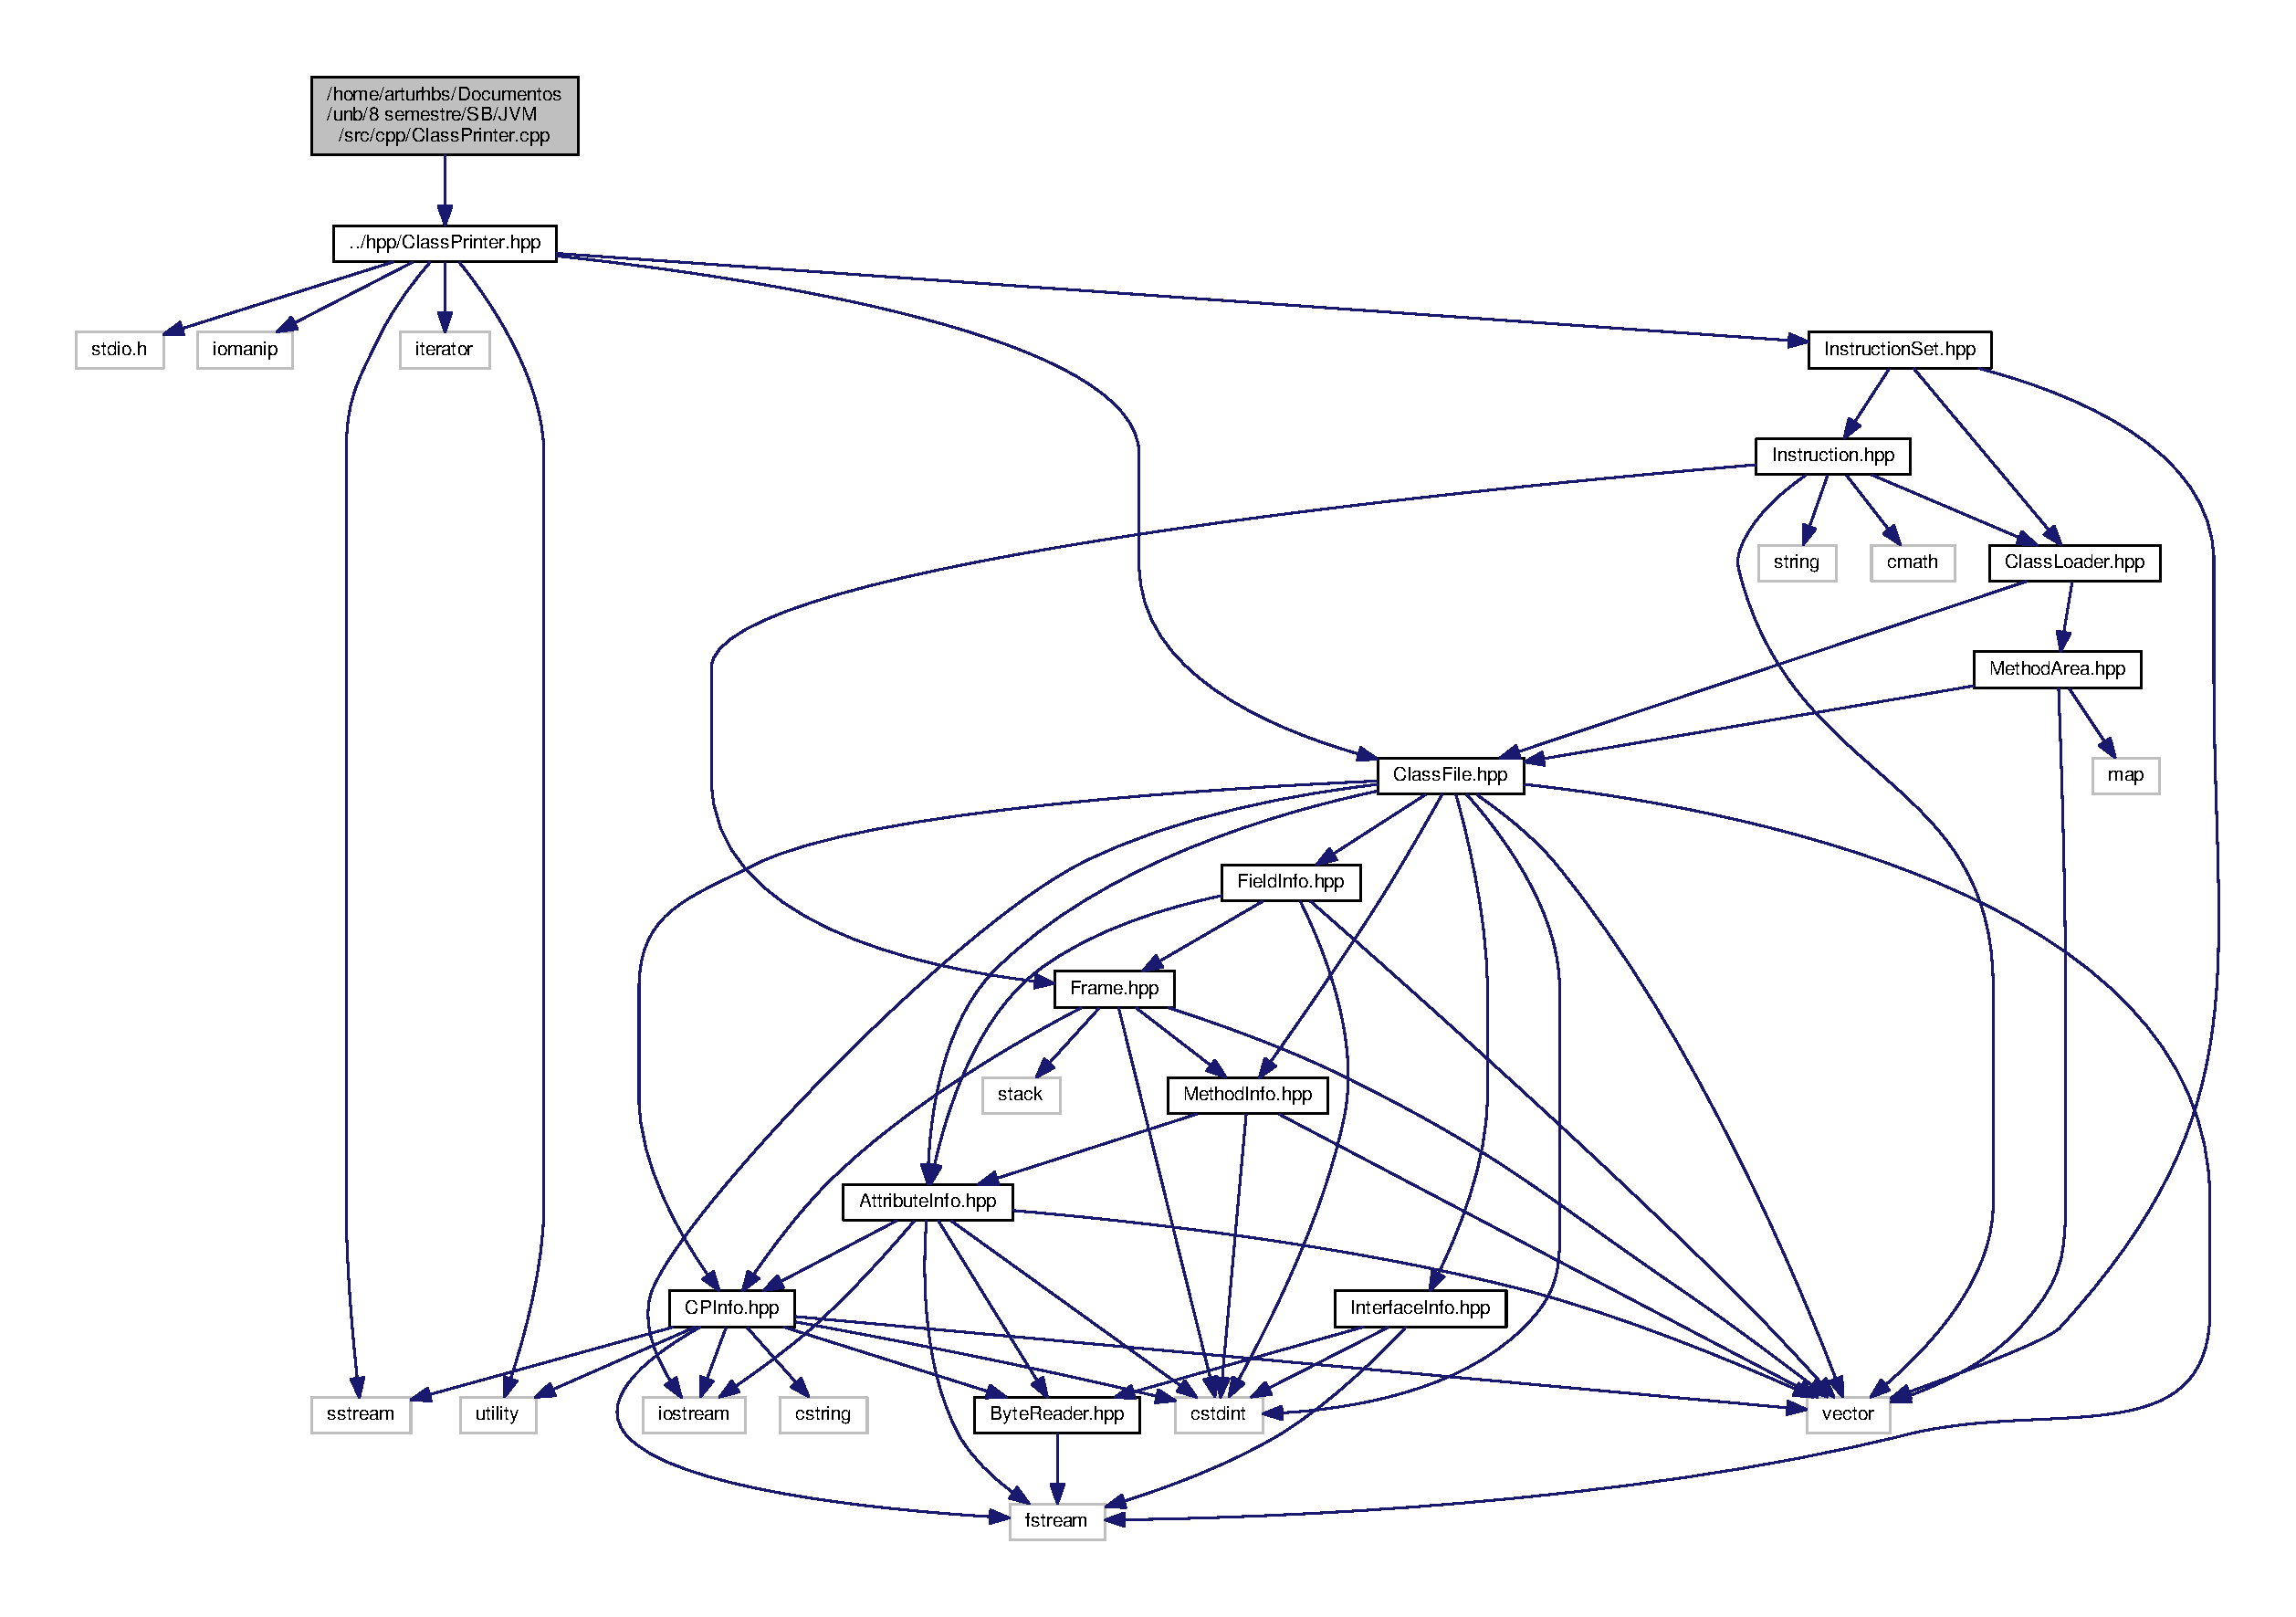
\includegraphics[width=350pt]{ClassPrinter_8cpp__incl}
\end{center}
\end{figure}


\subsection{Detailed Description}
Métodos que descrevem como será mostrado na tela. 

\begin{DoxyRefDesc}{Bug}
\item[\hyperlink{bug__bug000001}{Bug}]No known bugs. \end{DoxyRefDesc}

\hypertarget{AttributeInfo_8hpp}{}\section{/home/arturhbs/\+Documentos/unb/8 semestre/\+S\+B/\+J\+V\+M/src/hpp/\+Attribute\+Info.hpp File Reference}
\label{AttributeInfo_8hpp}\index{/home/arturhbs/\+Documentos/unb/8 semestre/\+S\+B/\+J\+V\+M/src/hpp/\+Attribute\+Info.\+hpp@{/home/arturhbs/\+Documentos/unb/8 semestre/\+S\+B/\+J\+V\+M/src/hpp/\+Attribute\+Info.\+hpp}}


Declarações das funções do \hyperlink{classAttributeInfo}{Attribute\+Info} para tratamento dos atributos do arquivo .class.  


{\ttfamily \#include $<$cstdint$>$}\\*
{\ttfamily \#include $<$vector$>$}\\*
{\ttfamily \#include $<$fstream$>$}\\*
{\ttfamily \#include $<$iostream$>$}\\*
{\ttfamily \#include \char`\"{}Byte\+Reader.\+hpp\char`\"{}}\\*
{\ttfamily \#include \char`\"{}C\+P\+Info.\+hpp\char`\"{}}\\*
Include dependency graph for Attribute\+Info.\+hpp\+:\nopagebreak
\begin{figure}[H]
\begin{center}
\leavevmode
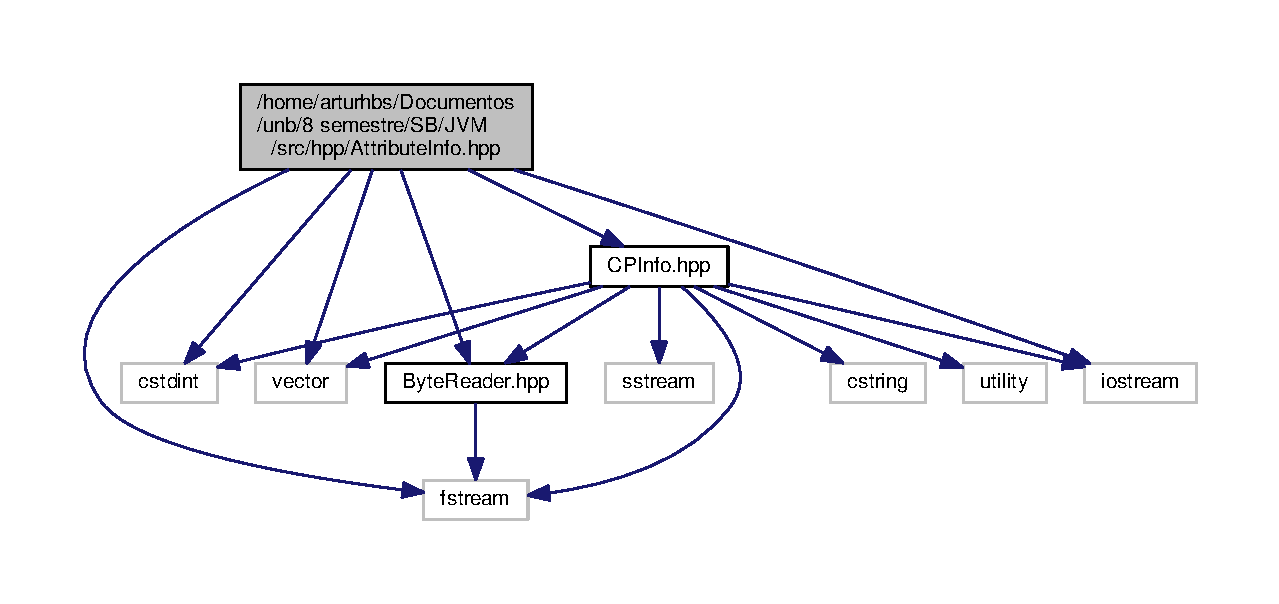
\includegraphics[width=350pt]{AttributeInfo_8hpp__incl}
\end{center}
\end{figure}
This graph shows which files directly or indirectly include this file\+:\nopagebreak
\begin{figure}[H]
\begin{center}
\leavevmode
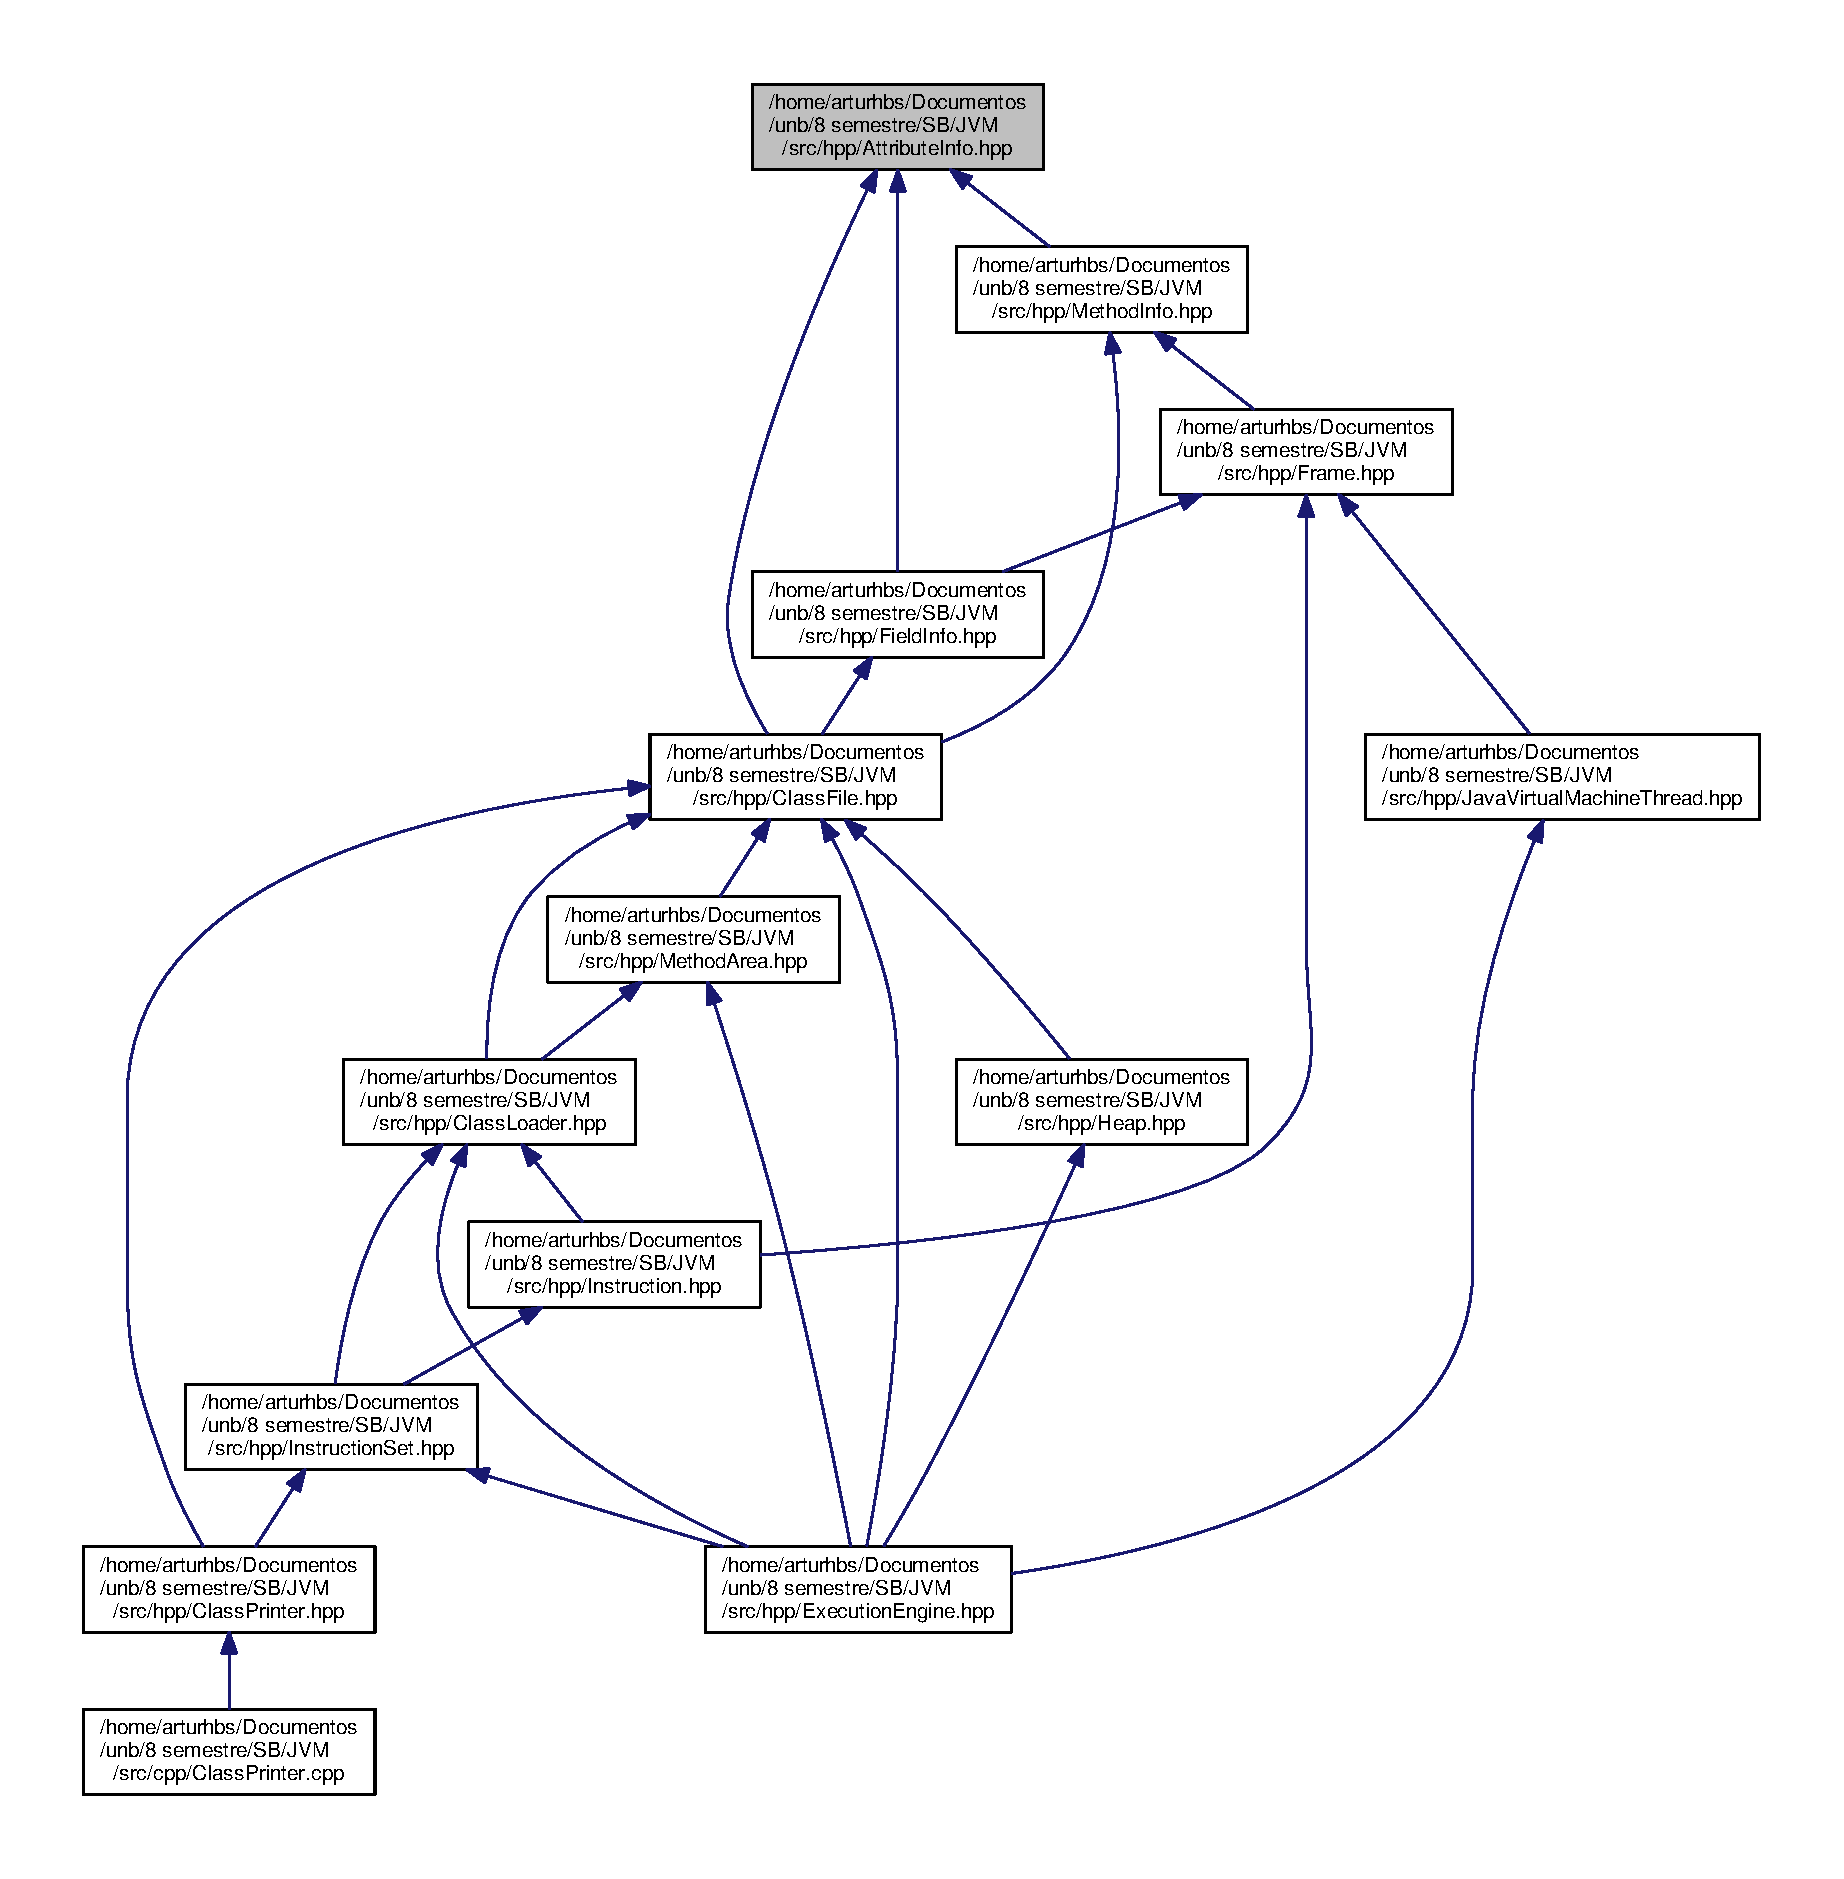
\includegraphics[width=350pt]{AttributeInfo_8hpp__dep__incl}
\end{center}
\end{figure}
\subsection*{Classes}
\begin{DoxyCompactItemize}
\item 
class \hyperlink{classConstantValueAttribute}{Constant\+Value\+Attribute}
\begin{DoxyCompactList}\small\item\em Classe que consiste em armazenar as informações dos index referentes aos atributos. \end{DoxyCompactList}\item 
class \hyperlink{classExceptionHandler}{Exception\+Handler}
\begin{DoxyCompactList}\small\item\em Classe que consiste em armazenar as informações das exceções. \end{DoxyCompactList}\item 
class \hyperlink{classCodeAttribute}{Code\+Attribute}
\begin{DoxyCompactList}\small\item\em Classe que consiste em armazenar as informações dos atributos. \end{DoxyCompactList}\item 
class \hyperlink{classExceptionsAttribute}{Exceptions\+Attribute}
\item 
class \hyperlink{classClassInfo}{Class\+Info}
\begin{DoxyCompactList}\small\item\em Classe que contém as informações gerais das classes. \end{DoxyCompactList}\item 
class \hyperlink{classInnerClassesAttribute}{Inner\+Classes\+Attribute}
\begin{DoxyCompactList}\small\item\em Classe que contém as informações dos atributos das classes. \end{DoxyCompactList}\item 
class \hyperlink{classSourceFileAttribute}{Source\+File\+Attribute}
\begin{DoxyCompactList}\small\item\em Classe que contém as informações do index do Source\+File. \end{DoxyCompactList}\item 
class \hyperlink{classLineNumber}{Line\+Number}
\item 
class \hyperlink{classLineNumberTableAttribute}{Line\+Number\+Table\+Attribute}
\item 
class \hyperlink{classLocalVariable}{Local\+Variable}
\item 
class \hyperlink{classLocalVariableTableAttribute}{Local\+Variable\+Table\+Attribute}
\item 
class \hyperlink{classAttributeInfo}{Attribute\+Info}
\end{DoxyCompactItemize}


\subsection{Detailed Description}
Declarações das funções do \hyperlink{classAttributeInfo}{Attribute\+Info} para tratamento dos atributos do arquivo .class. 

\begin{DoxyRefDesc}{Bug}
\item[\hyperlink{bug__bug000001}{Bug}]No known bugs. \end{DoxyRefDesc}

\hypertarget{ClassPrinter_8hpp}{}\section{/home/arturhbs/\+Documentos/unb/8 semestre/\+S\+B/\+J\+V\+M/src/hpp/\+Class\+Printer.hpp File Reference}
\label{ClassPrinter_8hpp}\index{/home/arturhbs/\+Documentos/unb/8 semestre/\+S\+B/\+J\+V\+M/src/hpp/\+Class\+Printer.\+hpp@{/home/arturhbs/\+Documentos/unb/8 semestre/\+S\+B/\+J\+V\+M/src/hpp/\+Class\+Printer.\+hpp}}


Declarações das funções que simular o programa jclasslib ao inserir um arquivo .class.  


{\ttfamily \#include $<$stdio.\+h$>$}\\*
{\ttfamily \#include $<$iomanip$>$}\\*
{\ttfamily \#include $<$sstream$>$}\\*
{\ttfamily \#include $<$iterator$>$}\\*
{\ttfamily \#include $<$utility$>$}\\*
{\ttfamily \#include \char`\"{}Class\+File.\+hpp\char`\"{}}\\*
{\ttfamily \#include \char`\"{}Instruction\+Set.\+hpp\char`\"{}}\\*
Include dependency graph for Class\+Printer.\+hpp\+:\nopagebreak
\begin{figure}[H]
\begin{center}
\leavevmode
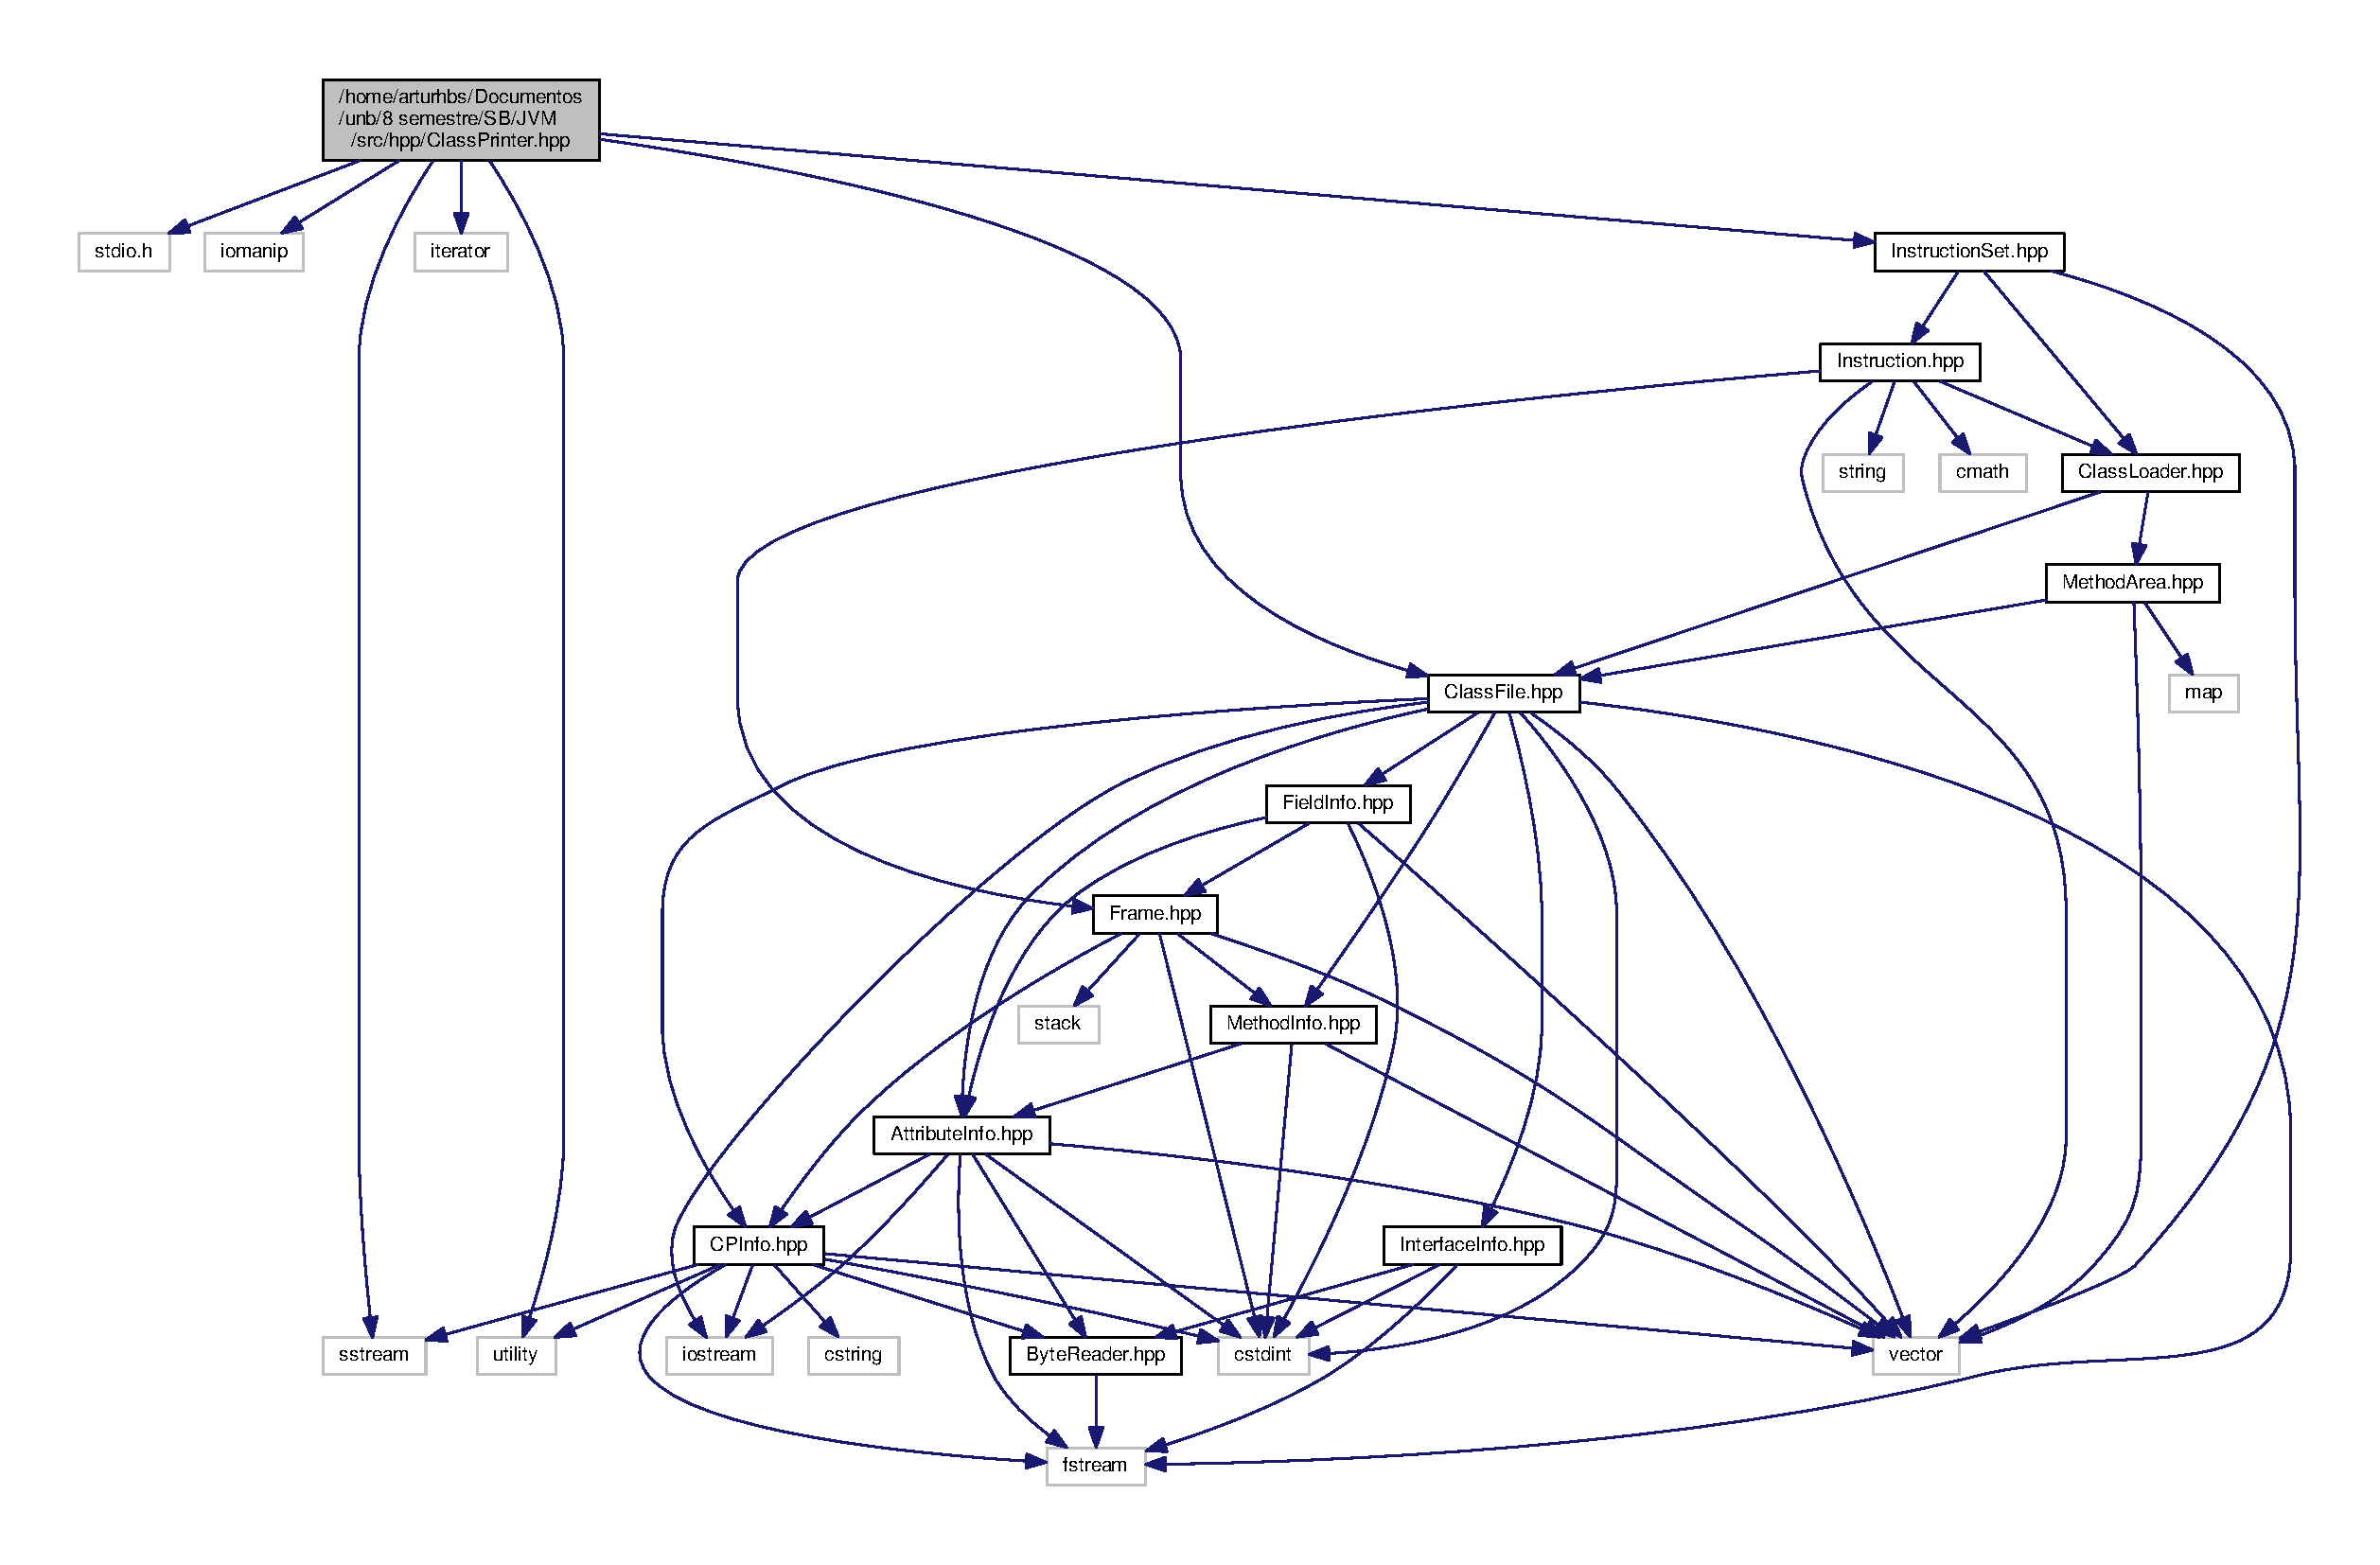
\includegraphics[width=350pt]{ClassPrinter_8hpp__incl}
\end{center}
\end{figure}
This graph shows which files directly or indirectly include this file\+:
\nopagebreak
\begin{figure}[H]
\begin{center}
\leavevmode
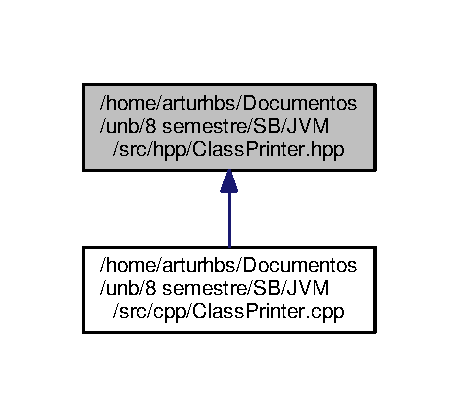
\includegraphics[width=220pt]{ClassPrinter_8hpp__dep__incl}
\end{center}
\end{figure}
\subsection*{Classes}
\begin{DoxyCompactItemize}
\item 
class \hyperlink{classClassPrinter}{Class\+Printer}
\begin{DoxyCompactList}\small\item\em classe que contém a chamada de todos os métodos que visam mostrar na tela os campos do class\+File; \end{DoxyCompactList}\end{DoxyCompactItemize}
\subsection*{Macros}
\begin{DoxyCompactItemize}
\item 
\#define {\bfseries C\+L\+E\+AR}~system(\char`\"{}clear\char`\"{});\hypertarget{ClassPrinter_8hpp_a611cc9b5f655508482f3d7a9751c182a}{}\label{ClassPrinter_8hpp_a611cc9b5f655508482f3d7a9751c182a}

\end{DoxyCompactItemize}


\subsection{Detailed Description}
Declarações das funções que simular o programa jclasslib ao inserir um arquivo .class. 

\begin{DoxyRefDesc}{Bug}
\item[\hyperlink{bug__bug000003}{Bug}]No known bugs. \end{DoxyRefDesc}

%--- End generated contents ---

% Index
\backmatter
\newpage
\phantomsection
\clearemptydoublepage
\addcontentsline{toc}{chapter}{Index}
\printindex

\end{document}
